\documentclass[twoside]{book}

% Packages required by doxygen
\usepackage{calc}
\usepackage{doxygen}
\usepackage{graphicx}
\usepackage[utf8]{inputenc}
\usepackage{makeidx}
\usepackage{multicol}
\usepackage{multirow}
\usepackage{textcomp}
\usepackage[table]{xcolor}

% Font selection
\usepackage[T1]{fontenc}
\usepackage{mathptmx}
\usepackage[scaled=.90]{helvet}
\usepackage{courier}
\usepackage{amssymb}
\usepackage{sectsty}
\renewcommand{\familydefault}{\sfdefault}
\allsectionsfont{%
  \fontseries{bc}\selectfont%
  \color{darkgray}%
}
\renewcommand{\DoxyLabelFont}{%
  \fontseries{bc}\selectfont%
  \color{darkgray}%
}

% Page & text layout
\usepackage{geometry}
\geometry{%
  a4paper,%
  top=2.5cm,%
  bottom=2.5cm,%
  left=2.5cm,%
  right=2.5cm%
}
\tolerance=750
\hfuzz=15pt
\hbadness=750
\setlength{\emergencystretch}{15pt}
\setlength{\parindent}{0cm}
\setlength{\parskip}{0.2cm}
\makeatletter
\renewcommand{\paragraph}{%
  \@startsection{paragraph}{4}{0ex}{-1.0ex}{1.0ex}{%
    \normalfont\normalsize\bfseries\SS@parafont%
  }%
}
\renewcommand{\subparagraph}{%
  \@startsection{subparagraph}{5}{0ex}{-1.0ex}{1.0ex}{%
    \normalfont\normalsize\bfseries\SS@subparafont%
  }%
}
\makeatother

% Headers & footers
\usepackage{fancyhdr}
\pagestyle{fancyplain}
\fancyhead[LE]{\fancyplain{}{\bfseries\thepage}}
\fancyhead[CE]{\fancyplain{}{}}
\fancyhead[RE]{\fancyplain{}{\bfseries\leftmark}}
\fancyhead[LO]{\fancyplain{}{\bfseries\rightmark}}
\fancyhead[CO]{\fancyplain{}{}}
\fancyhead[RO]{\fancyplain{}{\bfseries\thepage}}
\fancyfoot[LE]{\fancyplain{}{}}
\fancyfoot[CE]{\fancyplain{}{}}
\fancyfoot[RE]{\fancyplain{}{\bfseries\scriptsize Generated on Tue Jun 21 2016 21\-:39\-:49 for blend4php by Doxygen }}
\fancyfoot[LO]{\fancyplain{}{\bfseries\scriptsize Generated on Tue Jun 21 2016 21\-:39\-:49 for blend4php by Doxygen }}
\fancyfoot[CO]{\fancyplain{}{}}
\fancyfoot[RO]{\fancyplain{}{}}
\renewcommand{\footrulewidth}{0.4pt}
\renewcommand{\chaptermark}[1]{%
  \markboth{#1}{}%
}
\renewcommand{\sectionmark}[1]{%
  \markright{\thesection\ #1}%
}

% Indices & bibliography
\usepackage{natbib}
\usepackage[titles]{tocloft}
\setcounter{tocdepth}{3}
\setcounter{secnumdepth}{5}
\makeindex

% Hyperlinks (required, but should be loaded last)
\usepackage{ifpdf}
\ifpdf
  \usepackage[pdftex,pagebackref=true]{hyperref}
\else
  \usepackage[ps2pdf,pagebackref=true]{hyperref}
\fi
\hypersetup{%
  colorlinks=true,%
  linkcolor=blue,%
  citecolor=blue,%
  unicode%
}

% Custom commands
\newcommand{\clearemptydoublepage}{%
  \newpage{\pagestyle{empty}\cleardoublepage}%
}


%===== C O N T E N T S =====

\begin{document}

% Titlepage & ToC
\hypersetup{pageanchor=false}
\pagenumbering{roman}
\begin{titlepage}
\vspace*{7cm}
\begin{center}%
{\Large blend4php \\[1ex]\large v0.\-1 }\\
\vspace*{1cm}
{\large Generated by Doxygen 1.8.6}\\
\vspace*{0.5cm}
{\small Tue Jun 21 2016 21:39:49}\\
\end{center}
\end{titlepage}
\clearemptydoublepage
\tableofcontents
\clearemptydoublepage
\pagenumbering{arabic}
\hypersetup{pageanchor=true}

%--- Begin generated contents ---
\chapter{blend4php Documentation}
\label{index}\hypertarget{index}{}\hypertarget{index_intro_sec}{}\section{Introduction}\label{index_intro_sec}
The blend4php package is a P\-H\-P wrapper for the Galaxy A\-P\-I (\href{https://docs.galaxyproject.org/en/master/api_doc.html}{\tt https\-://docs.\-galaxyproject.\-org/en/master/api\-\_\-doc.\-html}). It follows the lead of Bio\-Blend (\href{https://bioblend.readthedocs.io/en/latest/}{\tt https\-://bioblend.\-readthedocs.\-io/en/latest/}) which provides a Python package for interacting with Galaxy and Cloud\-Man--hence the use of 'blend' in the name of this package. blend4php currently offers a partial implementation of the Galaxy A\-P\-I and includes support for datasets, data types, folder contents, folders, genomes, group roles, groups, group users, histories, history contents, jobs, libraries, library contents, requests, roles, search, tools, toolshed repositories, users, visualizations and workflows.

The motivation for development of this library is for integration with Tripal (\href{http://tripal.info}{\tt http\-://tripal.\-info}), an open-\/source toolkit for creation of online genomic, genetic and biological databases. Integration of Tripal and Galaxy will allow the community research databases to provide next-\/generation analytical tools to their users using Galaxy. However, this library was created independently of Tripal to support integration of any P\-H\-P application with Galaxy.\hypertarget{index_usage_sec}{}\section{Usage}\label{index_usage_sec}
To use blend4php, first include the galaxy.\-inc file in your program. For example\-:


\begin{DoxyCode}
require\_once(\textcolor{stringliteral}{'[blend4php installation dir]/galaxy.inc'})
\end{DoxyCode}


Where \mbox{[}blend4php installation dir\mbox{]} is where the blend4php package is installed.

To Connect to a galaxy instance\-:


\begin{DoxyCode}
$galaxy = \textcolor{keyword}{new} \hyperlink{classGalaxyInstance}{GalaxyInstance}($hostname, $port, $use\_https);
\end{DoxyCode}


The variables \$hostname and \$port should be the hostname (or I\-P address) and port number of the remote Galaxy server. If the server requires H\-T\-T\-Ps then \$use\-\_\-https should be T\-R\-U\-E.

To authenticate and retrieve the user's A\-P\-I key for future requests\-:


\begin{DoxyCode}
$success = $galaxy->authenticate($username, $password, $error)
\textcolor{keywordflow}{if} (!$success) \{
  \textcolor{comment}{// Handle a failed authentication.}
\}
\end{DoxyCode}


Where \$username is the name of the user on the remote Galaxy server and \$password is the user's password. The \$error variable will contain any error message if authentication fails. The function will return false if authentication fails.

If the A\-P\-I key for the user is already known, the authentication step can be skiped and the A\-P\-I key directly set\-:


\begin{DoxyCode}
$galaxy->setAPIKey($api\_key);
\end{DoxyCode}


Where the \$api\-\_\-key variable contains the A\-P\-I key of the user on the remote Galaxy server.

To interact with Galaxy regarding jobs, workflows, users, etc. Please review the Classes pages for each respective class.\hypertarget{index_error_sec}{}\section{Error Handling}\label{index_error_sec}
All functions in the blend4php library return F\-A\-L\-S\-E on failure. If failure occurs then the most recent error can be retrieved using the following\-:


\begin{DoxyCode}
$error = $galaxy->getError();
$emessage = $error[\textcolor{stringliteral}{'message'}]
$etype = $error[\textcolor{stringliteral}{'type'}]
\end{DoxyCode}


Alternatively, the message and type can be retrieved independently\-:


\begin{DoxyCode}
$emessage = $galaxy->getErrorMessage();
$etype = $galaxy->getErrorType();
\end{DoxyCode}
\hypertarget{index_funding_sec}{}\section{Funding}\label{index_funding_sec}
This work is supported by the U\-S National Science Foundation (N\-S\-F) award \#1443040, titled “\-C\-I\-F21 D\-I\-B\-B\-S\-: Tripal Gateway, a Platform for Next-\/\-Generation Data Analysis and Sharing.\-”\hypertarget{index_license_sec}{}\section{License}\label{index_license_sec}
blend4php is available under version 2 of the G\-N\-U General Public License 
\chapter{Hierarchical Index}
\section{Class Hierarchy}
This inheritance list is sorted roughly, but not completely, alphabetically\-:\begin{DoxyCompactList}
\item \contentsline{section}{Galaxy\-Datasets}{\pageref{classGalaxyDatasets}}{}
\item \contentsline{section}{Galaxy\-Datatypes}{\pageref{classGalaxyDatatypes}}{}
\item \contentsline{section}{Galaxy\-Error}{\pageref{classGalaxyError}}{}
\item \contentsline{section}{Galaxy\-Folder\-Contents}{\pageref{classGalaxyFolderContents}}{}
\item \contentsline{section}{Galaxy\-Folders}{\pageref{classGalaxyFolders}}{}
\item \contentsline{section}{Galaxy\-Genomes}{\pageref{classGalaxyGenomes}}{}
\item \contentsline{section}{Galaxy\-Group\-Roles}{\pageref{classGalaxyGroupRoles}}{}
\item \contentsline{section}{Galaxy\-Groups}{\pageref{classGalaxyGroups}}{}
\item \contentsline{section}{Galaxy\-Group\-Users}{\pageref{classGalaxyGroupUsers}}{}
\item \contentsline{section}{Galaxy\-Histories}{\pageref{classGalaxyHistories}}{}
\item \contentsline{section}{Galaxy\-History\-Contents}{\pageref{classGalaxyHistoryContents}}{}
\item \contentsline{section}{Galaxy\-H\-T\-T\-P\-Request}{\pageref{classGalaxyHTTPRequest}}{}
\begin{DoxyCompactList}
\item \contentsline{section}{Galaxy\-Instance}{\pageref{classGalaxyInstance}}{}
\end{DoxyCompactList}
\item \contentsline{section}{Galaxy\-Jobs}{\pageref{classGalaxyJobs}}{}
\item \contentsline{section}{Galaxy\-Libraries}{\pageref{classGalaxyLibraries}}{}
\item \contentsline{section}{Galaxy\-Library\-Contents}{\pageref{classGalaxyLibraryContents}}{}
\item \contentsline{section}{Galaxy\-Requests}{\pageref{classGalaxyRequests}}{}
\item \contentsline{section}{Galaxy\-Roles}{\pageref{classGalaxyRoles}}{}
\item \contentsline{section}{Galaxy\-Search}{\pageref{classGalaxySearch}}{}
\item \contentsline{section}{Galaxy\-Tools}{\pageref{classGalaxyTools}}{}
\item \contentsline{section}{Galaxy\-Tool\-Shed\-Repositories}{\pageref{classGalaxyToolShedRepositories}}{}
\item \contentsline{section}{Galaxy\-Users}{\pageref{classGalaxyUsers}}{}
\item \contentsline{section}{Galaxy\-Visualizations}{\pageref{classGalaxyVisualizations}}{}
\item \contentsline{section}{Galaxy\-Workflows}{\pageref{classGalaxyWorkflows}}{}
\end{DoxyCompactList}

\chapter{Class Index}
\section{Class List}
Here are the classes, structs, unions and interfaces with brief descriptions\+:\begin{DoxyCompactList}
\item\contentsline{section}{\hyperlink{classDatasets}{Datasets} }{\pageref{classDatasets}}{}
\item\contentsline{section}{\hyperlink{classDatatypes}{Datatypes} }{\pageref{classDatatypes}}{}
\item\contentsline{section}{\hyperlink{classFolderContents}{Folder\+Contents} }{\pageref{classFolderContents}}{}
\item\contentsline{section}{\hyperlink{classFolders}{Folders} }{\pageref{classFolders}}{}
\item\contentsline{section}{\hyperlink{classGalaxyInstance}{Galaxy\+Instance} }{\pageref{classGalaxyInstance}}{}
\item\contentsline{section}{\hyperlink{classGenomes}{Genomes} }{\pageref{classGenomes}}{}
\item\contentsline{section}{\hyperlink{classGroupRoles}{Group\+Roles} }{\pageref{classGroupRoles}}{}
\item\contentsline{section}{\hyperlink{classGroups}{Groups} }{\pageref{classGroups}}{}
\item\contentsline{section}{\hyperlink{classGroupUsers}{Group\+Users} }{\pageref{classGroupUsers}}{}
\item\contentsline{section}{\hyperlink{classHistories}{Histories} }{\pageref{classHistories}}{}
\item\contentsline{section}{\hyperlink{classHistoryContents}{History\+Contents} }{\pageref{classHistoryContents}}{}
\item\contentsline{section}{\hyperlink{classHTTPRequest}{H\+T\+T\+P\+Request} }{\pageref{classHTTPRequest}}{}
\item\contentsline{section}{\hyperlink{classJobs}{Jobs} }{\pageref{classJobs}}{}
\item\contentsline{section}{\hyperlink{classLibraries}{Libraries} }{\pageref{classLibraries}}{}
\item\contentsline{section}{\hyperlink{classLibraryContents}{Library\+Contents} }{\pageref{classLibraryContents}}{}
\item\contentsline{section}{\hyperlink{classRequestError}{Request\+Error} }{\pageref{classRequestError}}{}
\item\contentsline{section}{\hyperlink{classRequests}{Requests} }{\pageref{classRequests}}{}
\item\contentsline{section}{\hyperlink{classRoles}{Roles} }{\pageref{classRoles}}{}
\item\contentsline{section}{\hyperlink{classSearch}{Search} }{\pageref{classSearch}}{}
\item\contentsline{section}{\hyperlink{classTools}{Tools} }{\pageref{classTools}}{}
\item\contentsline{section}{\hyperlink{classToolShedRepositories}{Tool\+Shed\+Repositories} }{\pageref{classToolShedRepositories}}{}
\item\contentsline{section}{\hyperlink{classUsers}{Users} }{\pageref{classUsers}}{}
\item\contentsline{section}{\hyperlink{classVisualizations}{Visualizations} }{\pageref{classVisualizations}}{}
\item\contentsline{section}{\hyperlink{classWorkflows}{Workflows} }{\pageref{classWorkflows}}{}
\end{DoxyCompactList}

\chapter{Class Documentation}
\hypertarget{classGalaxyDatasets}{\section{Galaxy\-Datasets Class Reference}
\label{classGalaxyDatasets}\index{Galaxy\-Datasets@{Galaxy\-Datasets}}
}
\subsection*{Public Member Functions}
\begin{DoxyCompactItemize}
\item 
\hyperlink{classGalaxyDatasets_a397cff30313f1f6b8e1b28a45c4aea40}{\-\_\-\-\_\-construct} (\$galaxy)
\item 
\hyperlink{classGalaxyDatasets_a0cc78f7d1b21da1522f04e79e1e06b13}{converted} (\$params)
\item 
\hyperlink{classGalaxyDatasets_af06f7b78544fab66c089bd32843a4401}{display} (\$params)
\item 
\hyperlink{classGalaxyDatasets_ad1e98fbcd098cd094f5251b1c73875ac}{index} ()
\item 
\hyperlink{classGalaxyDatasets_a3c4e140d02e38101c256c995b41cdc53}{show} (\$params)
\end{DoxyCompactItemize}


\subsection{Constructor \& Destructor Documentation}
\hypertarget{classGalaxyDatasets_a397cff30313f1f6b8e1b28a45c4aea40}{\index{Galaxy\-Datasets@{Galaxy\-Datasets}!\-\_\-\-\_\-construct@{\-\_\-\-\_\-construct}}
\index{\-\_\-\-\_\-construct@{\-\_\-\-\_\-construct}!GalaxyDatasets@{Galaxy\-Datasets}}
\subsubsection[{\-\_\-\-\_\-construct}]{\setlength{\rightskip}{0pt plus 5cm}Galaxy\-Datasets\-::\-\_\-\-\_\-construct (
\begin{DoxyParamCaption}
\item[{}]{\$galaxy}
\end{DoxyParamCaption}
)}}\label{classGalaxyDatasets_a397cff30313f1f6b8e1b28a45c4aea40}
The Data\-Sets constructor.


\begin{DoxyParams}[1]{Parameters}
\hyperlink{classGalaxyInstance}{Galaxy\-Instance} & {\em \$galaxy} & A \hyperlink{classGalaxyInstance}{Galaxy\-Instance} object.\\
\hline
\end{DoxyParams}
\begin{DoxyReturn}{Returns}
An instance of a Data\-Set object. 
\end{DoxyReturn}


\subsection{Member Function Documentation}
\hypertarget{classGalaxyDatasets_a0cc78f7d1b21da1522f04e79e1e06b13}{\index{Galaxy\-Datasets@{Galaxy\-Datasets}!converted@{converted}}
\index{converted@{converted}!GalaxyDatasets@{Galaxy\-Datasets}}
\subsubsection[{converted}]{\setlength{\rightskip}{0pt plus 5cm}Galaxy\-Datasets\-::converted (
\begin{DoxyParamCaption}
\item[{}]{\$params}
\end{DoxyParamCaption}
)}}\label{classGalaxyDatasets_a0cc78f7d1b21da1522f04e79e1e06b13}
Retreive information about datasets made by converting to a new file format.

Corresponds to the galaxy A\-P\-I function at\-: G\-E\-T /api/datasets/\{dataset\-\_\-id\}/converted/\{ext\}


\begin{DoxyParams}{Parameters}
{\em \$params} & An associative array containing the input parameters for this function. The following parameters are available\-:\\
\hline
\end{DoxyParams}

\begin{DoxyItemize}
\item dataset\-\_\-id\-: The dataset id of the information to pull. Can be obtained from this function's \hyperlink{classGalaxyDatasets_af06f7b78544fab66c089bd32843a4401}{display()}.
\item extension (optional)\-: If supplied this will look at the file extension.
\end{DoxyItemize}

\begin{DoxyReturn}{Returns}
An array containing information about the matching dataset(s). 
\end{DoxyReturn}
\hypertarget{classGalaxyDatasets_af06f7b78544fab66c089bd32843a4401}{\index{Galaxy\-Datasets@{Galaxy\-Datasets}!display@{display}}
\index{display@{display}!GalaxyDatasets@{Galaxy\-Datasets}}
\subsubsection[{display}]{\setlength{\rightskip}{0pt plus 5cm}Galaxy\-Datasets\-::display (
\begin{DoxyParamCaption}
\item[{}]{\$params}
\end{DoxyParamCaption}
)}}\label{classGalaxyDatasets_af06f7b78544fab66c089bd32843a4401}
Retreives a list of datasets associated with a given history.

Corresponds to the Galaxy Api method and path\-: G\-E\-T /api/histories/\{encoded\-\_\-history\-\_\-id\}/contents/\{encoded\-\_\-content\-\_\-id\}/display history content (dataset).


\begin{DoxyParams}{Parameters}
{\em \$params} & An associative array containing the input parameters for this function. The following parameters are available\-:\\
\hline
\end{DoxyParams}

\begin{DoxyItemize}
\item hist\-\_\-id\-: The history id of the datasets to find.
\item hist\-\_\-content\-\_\-id\-: The specified history content's dataset(s) to list. Please see the History\-Contents class to obtain the history content id
\end{DoxyItemize}

\begin{DoxyReturn}{Returns}
An array containing information about the matching dataset(s). 
\end{DoxyReturn}
\hypertarget{classGalaxyDatasets_ad1e98fbcd098cd094f5251b1c73875ac}{\index{Galaxy\-Datasets@{Galaxy\-Datasets}!index@{index}}
\index{index@{index}!GalaxyDatasets@{Galaxy\-Datasets}}
\subsubsection[{index}]{\setlength{\rightskip}{0pt plus 5cm}Galaxy\-Datasets\-::index (
\begin{DoxyParamCaption}
{}
\end{DoxyParamCaption}
)}}\label{classGalaxyDatasets_ad1e98fbcd098cd094f5251b1c73875ac}
Retreives a list of all datasets.

Currently not supported by the Galaxy A\-P\-I \hypertarget{classGalaxyDatasets_a3c4e140d02e38101c256c995b41cdc53}{\index{Galaxy\-Datasets@{Galaxy\-Datasets}!show@{show}}
\index{show@{show}!GalaxyDatasets@{Galaxy\-Datasets}}
\subsubsection[{show}]{\setlength{\rightskip}{0pt plus 5cm}Galaxy\-Datasets\-::show (
\begin{DoxyParamCaption}
\item[{}]{\$params}
\end{DoxyParamCaption}
)}}\label{classGalaxyDatasets_a3c4e140d02e38101c256c995b41cdc53}
Retreives detailed content on a specific dataset.

Corresponds to the Galaxy Api function and path\-: G\-E\-T /api/datasets/\{encoded\-\_\-dataset\-\_\-id\}


\begin{DoxyParams}{Parameters}
{\em \$params} & An associative array containing the input parameters for this function. The following parameters are available\-:\\
\hline
\end{DoxyParams}

\begin{DoxyItemize}
\item dataset\-\_\-id\-: The dataset\-\_\-id's information that the function is to retreive. To obtain the dataset id, please use the Display function.
\end{DoxyItemize}

\begin{DoxyReturn}{Returns}
An array containing information about the matching dataset. 
\end{DoxyReturn}


The documentation for this class was generated from the following file\-:\begin{DoxyCompactItemize}
\item 
Data\-Sets.\-inc\end{DoxyCompactItemize}

\hypertarget{classGalaxyDatatypes}{\section{Galaxy\-Datatypes Class Reference}
\label{classGalaxyDatatypes}\index{Galaxy\-Datatypes@{Galaxy\-Datatypes}}
}
\subsection*{Public Member Functions}
\begin{DoxyCompactItemize}
\item 
\hyperlink{classGalaxyDatatypes_aeb7dee89c76290fd8767b91d63ba872c}{\-\_\-\-\_\-construct} (\hyperlink{classGalaxyInstance}{Galaxy\-Instance} \$galaxy)
\item 
\hyperlink{classGalaxyDatatypes_a985aa52b7839d1fbfa087f3239180c57}{sniffers} ()
\item 
\hyperlink{classGalaxyDatatypes_a1a7972aee88fae45b2156feb39827b0d}{converters} ()
\item 
\hyperlink{classGalaxyDatatypes_a4e5f73d90ee19f5042f8a07bec045d04}{edam\-Formats} ()
\item 
\hyperlink{classGalaxyDatatypes_aaad2077b4324f2241c5e3c3619fb2dd8}{mapping} ()
\item 
\hyperlink{classGalaxyDatatypes_afa23ec4543ef41cae7b07ea2c03558ae}{index} ()
\end{DoxyCompactItemize}


\subsection{Constructor \& Destructor Documentation}
\hypertarget{classGalaxyDatatypes_aeb7dee89c76290fd8767b91d63ba872c}{\index{Galaxy\-Datatypes@{Galaxy\-Datatypes}!\-\_\-\-\_\-construct@{\-\_\-\-\_\-construct}}
\index{\-\_\-\-\_\-construct@{\-\_\-\-\_\-construct}!GalaxyDatatypes@{Galaxy\-Datatypes}}
\subsubsection[{\-\_\-\-\_\-construct}]{\setlength{\rightskip}{0pt plus 5cm}Galaxy\-Datatypes\-::\-\_\-\-\_\-construct (
\begin{DoxyParamCaption}
\item[{{\bf Galaxy\-Instance}}]{\$galaxy}
\end{DoxyParamCaption}
)}}\label{classGalaxyDatatypes_aeb7dee89c76290fd8767b91d63ba872c}
The Data\-Types constructor.


\begin{DoxyParams}[1]{Parameters}
\hyperlink{classGalaxyInstance}{Galaxy\-Instance} & {\em \$galaxy} & A \hyperlink{classGalaxyInstance}{Galaxy\-Instance} object.\\
\hline
\end{DoxyParams}
\begin{DoxyReturn}{Returns}
An instance of a Datatypes object. 
\end{DoxyReturn}


\subsection{Member Function Documentation}
\hypertarget{classGalaxyDatatypes_a1a7972aee88fae45b2156feb39827b0d}{\index{Galaxy\-Datatypes@{Galaxy\-Datatypes}!converters@{converters}}
\index{converters@{converters}!GalaxyDatatypes@{Galaxy\-Datatypes}}
\subsubsection[{converters}]{\setlength{\rightskip}{0pt plus 5cm}Galaxy\-Datatypes\-::converters (
\begin{DoxyParamCaption}
{}
\end{DoxyParamCaption}
)}}\label{classGalaxyDatatypes_a1a7972aee88fae45b2156feb39827b0d}
Retreive a list of all datatype converters.

Corresponds to the Galaxy A\-P\-I/\-Path\-: G\-E\-T /api/datatypes/converters

\begin{DoxyReturn}{Returns}
An array containing converters of all datatypes 
\end{DoxyReturn}
\hypertarget{classGalaxyDatatypes_a4e5f73d90ee19f5042f8a07bec045d04}{\index{Galaxy\-Datatypes@{Galaxy\-Datatypes}!edam\-Formats@{edam\-Formats}}
\index{edam\-Formats@{edam\-Formats}!GalaxyDatatypes@{Galaxy\-Datatypes}}
\subsubsection[{edam\-Formats}]{\setlength{\rightskip}{0pt plus 5cm}Galaxy\-Datatypes\-::edam\-Formats (
\begin{DoxyParamCaption}
{}
\end{DoxyParamCaption}
)}}\label{classGalaxyDatatypes_a4e5f73d90ee19f5042f8a07bec045d04}
Retreive a list of all datatypes in the edam format.

Corresponds to the Galaxy A\-P\-I/\-Path\-: G\-E\-T /api/datatypes/edam\-\_\-formats

\begin{DoxyReturn}{Returns}
An array containing all datatypes in edam\-\_\-format. 
\end{DoxyReturn}
\hypertarget{classGalaxyDatatypes_afa23ec4543ef41cae7b07ea2c03558ae}{\index{Galaxy\-Datatypes@{Galaxy\-Datatypes}!index@{index}}
\index{index@{index}!GalaxyDatatypes@{Galaxy\-Datatypes}}
\subsubsection[{index}]{\setlength{\rightskip}{0pt plus 5cm}Galaxy\-Datatypes\-::index (
\begin{DoxyParamCaption}
{}
\end{DoxyParamCaption}
)}}\label{classGalaxyDatatypes_afa23ec4543ef41cae7b07ea2c03558ae}
Retreive a list of all datatypes

Corresponds to the Galaxy A\-P\-I/\-Path\-: G\-E\-T /api/datatypes/

\begin{DoxyReturn}{Returns}
An array containing all datatypes 
\end{DoxyReturn}
\hypertarget{classGalaxyDatatypes_aaad2077b4324f2241c5e3c3619fb2dd8}{\index{Galaxy\-Datatypes@{Galaxy\-Datatypes}!mapping@{mapping}}
\index{mapping@{mapping}!GalaxyDatatypes@{Galaxy\-Datatypes}}
\subsubsection[{mapping}]{\setlength{\rightskip}{0pt plus 5cm}Galaxy\-Datatypes\-::mapping (
\begin{DoxyParamCaption}
{}
\end{DoxyParamCaption}
)}}\label{classGalaxyDatatypes_aaad2077b4324f2241c5e3c3619fb2dd8}
Retreive a list of all datatypes in mapping.

Corresponds to the Galaxy A\-P\-I/\-Path\-: G\-E\-T /api/datatypes/mapping.

\begin{DoxyReturn}{Returns}
An array containing all datatypes in mapping. 
\end{DoxyReturn}
\hypertarget{classGalaxyDatatypes_a985aa52b7839d1fbfa087f3239180c57}{\index{Galaxy\-Datatypes@{Galaxy\-Datatypes}!sniffers@{sniffers}}
\index{sniffers@{sniffers}!GalaxyDatatypes@{Galaxy\-Datatypes}}
\subsubsection[{sniffers}]{\setlength{\rightskip}{0pt plus 5cm}Galaxy\-Datatypes\-::sniffers (
\begin{DoxyParamCaption}
{}
\end{DoxyParamCaption}
)}}\label{classGalaxyDatatypes_a985aa52b7839d1fbfa087f3239180c57}
Retreive a list of all datatype sniffers.

Corresponds to the Galaxy A\-P\-I/\-Path\-: G\-E\-T /api/datatypes/sniffers

\begin{DoxyReturn}{Returns}
An array containing sniffers of all datatypes 
\end{DoxyReturn}


The documentation for this class was generated from the following file\-:\begin{DoxyCompactItemize}
\item 
Data\-Types.\-inc\end{DoxyCompactItemize}

\hypertarget{classGalaxyError}{\section{Galaxy\-Error Class Reference}
\label{classGalaxyError}\index{Galaxy\-Error@{Galaxy\-Error}}
}
\subsection*{Public Member Functions}
\begin{DoxyCompactItemize}
\item 
\hyperlink{classGalaxyError_af945b84be50ec41616a4c0b40e170bb9}{\-\_\-\-\_\-construct} ()
\item 
\hyperlink{classGalaxyError_a028ee131e1f68da22c29e510b405e0a7}{get\-Error} ()
\item 
\hyperlink{classGalaxyError_a1f1ec54a9bcb9520dbaa7abc3e163824}{get\-Error\-Message} ()
\item 
\hyperlink{classGalaxyError_a2e680e1a6475af8dfbcb6d1f07254f8c}{get\-Error\-Type} ()
\item 
\hyperlink{classGalaxyError_a4c3312a17a9f150a6a64b44b345a6143}{set\-Error} (\$type, \$message)
\end{DoxyCompactItemize}


\subsection{Constructor \& Destructor Documentation}
\hypertarget{classGalaxyError_af945b84be50ec41616a4c0b40e170bb9}{\index{Galaxy\-Error@{Galaxy\-Error}!\-\_\-\-\_\-construct@{\-\_\-\-\_\-construct}}
\index{\-\_\-\-\_\-construct@{\-\_\-\-\_\-construct}!GalaxyError@{Galaxy\-Error}}
\subsubsection[{\-\_\-\-\_\-construct}]{\setlength{\rightskip}{0pt plus 5cm}Galaxy\-Error\-::\-\_\-\-\_\-construct (
\begin{DoxyParamCaption}
{}
\end{DoxyParamCaption}
)}}\label{classGalaxyError_af945b84be50ec41616a4c0b40e170bb9}
Constructor. 

\subsection{Member Function Documentation}
\hypertarget{classGalaxyError_a028ee131e1f68da22c29e510b405e0a7}{\index{Galaxy\-Error@{Galaxy\-Error}!get\-Error@{get\-Error}}
\index{get\-Error@{get\-Error}!GalaxyError@{Galaxy\-Error}}
\subsubsection[{get\-Error}]{\setlength{\rightskip}{0pt plus 5cm}Galaxy\-Error\-::get\-Error (
\begin{DoxyParamCaption}
{}
\end{DoxyParamCaption}
)}}\label{classGalaxyError_a028ee131e1f68da22c29e510b405e0a7}
Retrieves the most recent error.

The error message uses the key 'message' and the type uses the key 'type'. The following is a list of error types and their meaning\-:


\begin{DoxyItemize}
\item A\-P\-I\-: The blend4php A\-P\-I functions have been improperly used
\item Galaxy\-: The Galaxy server indicated an error.
\item H\-T\-T\-P\-: An error occured using the R\-E\-S\-T H\-T\-T\-P protocols (e.\-g. P\-U\-T, P\-O\-S\-T, G\-E\-T, P\-A\-T\-C\-H, D\-E\-L\-E\-T\-E).
\item F\-I\-L\-E\-: An error occured saving a download file from Galaxy.
\end{DoxyItemize}

\begin{DoxyReturn}{Returns}
An associative array containing both the 'type' and 'message' for the error. 
\end{DoxyReturn}
\hypertarget{classGalaxyError_a1f1ec54a9bcb9520dbaa7abc3e163824}{\index{Galaxy\-Error@{Galaxy\-Error}!get\-Error\-Message@{get\-Error\-Message}}
\index{get\-Error\-Message@{get\-Error\-Message}!GalaxyError@{Galaxy\-Error}}
\subsubsection[{get\-Error\-Message}]{\setlength{\rightskip}{0pt plus 5cm}Galaxy\-Error\-::get\-Error\-Message (
\begin{DoxyParamCaption}
{}
\end{DoxyParamCaption}
)}}\label{classGalaxyError_a1f1ec54a9bcb9520dbaa7abc3e163824}
Retrieves the most recent error message.

\begin{DoxyReturn}{Returns}
A string containing the error message. 
\end{DoxyReturn}
\hypertarget{classGalaxyError_a2e680e1a6475af8dfbcb6d1f07254f8c}{\index{Galaxy\-Error@{Galaxy\-Error}!get\-Error\-Type@{get\-Error\-Type}}
\index{get\-Error\-Type@{get\-Error\-Type}!GalaxyError@{Galaxy\-Error}}
\subsubsection[{get\-Error\-Type}]{\setlength{\rightskip}{0pt plus 5cm}Galaxy\-Error\-::get\-Error\-Type (
\begin{DoxyParamCaption}
{}
\end{DoxyParamCaption}
)}}\label{classGalaxyError_a2e680e1a6475af8dfbcb6d1f07254f8c}
Retrieves the most recent error type.

The following is a list of error types and their meaning\-:


\begin{DoxyItemize}
\item A\-P\-I\-: The blend4php A\-P\-I functions have been improperly used
\item Galaxy\-: The Galaxy server indicated an error.
\item H\-T\-T\-P\-: An error occured using the R\-E\-S\-T H\-T\-T\-P protocols (e.\-g. P\-U\-T, P\-O\-S\-T, G\-E\-T, P\-A\-T\-C\-H, D\-E\-L\-E\-T\-E).
\item F\-I\-L\-E\-: An error occured saving a download file from Galaxy.
\end{DoxyItemize}

\begin{DoxyReturn}{Returns}
A string indicating the type of error. 
\end{DoxyReturn}
\hypertarget{classGalaxyError_a4c3312a17a9f150a6a64b44b345a6143}{\index{Galaxy\-Error@{Galaxy\-Error}!set\-Error@{set\-Error}}
\index{set\-Error@{set\-Error}!GalaxyError@{Galaxy\-Error}}
\subsubsection[{set\-Error}]{\setlength{\rightskip}{0pt plus 5cm}Galaxy\-Error\-::set\-Error (
\begin{DoxyParamCaption}
\item[{}]{\$type, }
\item[{}]{\$message}
\end{DoxyParamCaption}
)}}\label{classGalaxyError_a4c3312a17a9f150a6a64b44b345a6143}
Set's the error type and message.

The following is a list of error types and their meaning\-:


\begin{DoxyItemize}
\item A\-P\-I\-: The blend4php A\-P\-I functions have been improperly used
\item Galaxy\-: The Galaxy server indicated an error.
\item H\-T\-T\-P\-: An error occured using the R\-E\-S\-T H\-T\-T\-P protocols (e.\-g. P\-U\-T, P\-O\-S\-T, G\-E\-T, P\-A\-T\-C\-H, D\-E\-L\-E\-T\-E).
\item F\-I\-L\-E\-: An error occured saving a download file from Galaxy.
\end{DoxyItemize}


\begin{DoxyParams}{Parameters}
{\em \$type} & The type of error. \\
\hline
{\em \$message} & The error message. \\
\hline
\end{DoxyParams}


The documentation for this class was generated from the following file\-:\begin{DoxyCompactItemize}
\item 
Error.\-inc\end{DoxyCompactItemize}

\hypertarget{classGalaxyFolderContents}{\section{Galaxy\-Folder\-Contents Class Reference}
\label{classGalaxyFolderContents}\index{Galaxy\-Folder\-Contents@{Galaxy\-Folder\-Contents}}
}
\subsection*{Public Member Functions}
\begin{DoxyCompactItemize}
\item 
\hyperlink{classGalaxyFolderContents_a80b2fee2628123ffd888a1bdf6e74e37}{\-\_\-\-\_\-construct} (\hyperlink{classGalaxyInstance}{Galaxy\-Instance} \$galaxy)
\item 
\hyperlink{classGalaxyFolderContents_a6a59567a3ceb326db7c14337ea91a097}{index} (\$params)
\item 
\hyperlink{classGalaxyFolderContents_a8497234cbbcaa30eccdeaa7d95131775}{create} (\$params)
\item 
\hyperlink{classGalaxyFolderContents_ad18d388119d9f1cdf24ca5b2cc613600}{show} (\$params)
\item 
\hyperlink{classGalaxyFolderContents_a0836714c15c9279d0c49988fb56726ea}{update} (\$params)
\end{DoxyCompactItemize}


\subsection{Constructor \& Destructor Documentation}
\hypertarget{classGalaxyFolderContents_a80b2fee2628123ffd888a1bdf6e74e37}{\index{Galaxy\-Folder\-Contents@{Galaxy\-Folder\-Contents}!\-\_\-\-\_\-construct@{\-\_\-\-\_\-construct}}
\index{\-\_\-\-\_\-construct@{\-\_\-\-\_\-construct}!GalaxyFolderContents@{Galaxy\-Folder\-Contents}}
\subsubsection[{\-\_\-\-\_\-construct}]{\setlength{\rightskip}{0pt plus 5cm}Galaxy\-Folder\-Contents\-::\-\_\-\-\_\-construct (
\begin{DoxyParamCaption}
\item[{{\bf Galaxy\-Instance}}]{\$galaxy}
\end{DoxyParamCaption}
)}}\label{classGalaxyFolderContents_a80b2fee2628123ffd888a1bdf6e74e37}
The Folder\-Contents constructor.


\begin{DoxyParams}[1]{Parameters}
\hyperlink{classGalaxyInstance}{Galaxy\-Instance} & {\em \$galaxy} & A \hyperlink{classGalaxyInstance}{Galaxy\-Instance} object.\\
\hline
\end{DoxyParams}
\begin{DoxyReturn}{Returns}
An instance of a Folder\-Contents object. 
\end{DoxyReturn}


\subsection{Member Function Documentation}
\hypertarget{classGalaxyFolderContents_a8497234cbbcaa30eccdeaa7d95131775}{\index{Galaxy\-Folder\-Contents@{Galaxy\-Folder\-Contents}!create@{create}}
\index{create@{create}!GalaxyFolderContents@{Galaxy\-Folder\-Contents}}
\subsubsection[{create}]{\setlength{\rightskip}{0pt plus 5cm}Galaxy\-Folder\-Contents\-::create (
\begin{DoxyParamCaption}
\item[{}]{\$params}
\end{DoxyParamCaption}
)}}\label{classGalaxyFolderContents_a8497234cbbcaa30eccdeaa7d95131775}
Create a new content for specified folder

Corresponds to the Galaxy A\-P\-I/path at\-: P\-O\-S\-T /api/folders/\{folder\-\_\-id\}/contents


\begin{DoxyParams}{Parameters}
{\em \$params} & An associative array containing the input parameters for this function. The following parameters are available\-:\\
\hline
\end{DoxyParams}

\begin{DoxyItemize}
\item parent\-\_\-folder\-\_\-id\-: The parent folder of the new item. To obtain id, see the \hyperlink{classGalaxyFolderContents_a6a59567a3ceb326db7c14337ea91a097}{index()} function in the Folder class.
\item from\-\_\-hda\-\_\-id (Optional)\-: The id of an accessible H\-D\-A to into the library. To obtain this id, see \hyperlink{classGalaxyFolderContents_a6a59567a3ceb326db7c14337ea91a097}{index()} in History\-Contents class.
\item ldda\-\_\-messge (Optional)\-: Any message to send along with the Library\-Dataset\-Association.
\item extented\-\_\-metadata (Optional)\-: Sub-\/dictionary containing any extended metadata to associate with the item.
\end{DoxyItemize}

\begin{DoxyReturn}{Returns}
An array containing the newly created folder content. 
\end{DoxyReturn}
\hypertarget{classGalaxyFolderContents_a6a59567a3ceb326db7c14337ea91a097}{\index{Galaxy\-Folder\-Contents@{Galaxy\-Folder\-Contents}!index@{index}}
\index{index@{index}!GalaxyFolderContents@{Galaxy\-Folder\-Contents}}
\subsubsection[{index}]{\setlength{\rightskip}{0pt plus 5cm}Galaxy\-Folder\-Contents\-::index (
\begin{DoxyParamCaption}
\item[{}]{\$params}
\end{DoxyParamCaption}
)}}\label{classGalaxyFolderContents_a6a59567a3ceb326db7c14337ea91a097}
Displays all the contents of a folder.

Corresponds to the Galaxy A\-P\-I/path\-: G\-E\-T /api/folders/\-F\{folder\-\_\-id\}/contents.


\begin{DoxyParams}{Parameters}
{\em \$params} & An associative array containing the input parameters for this function. The following parameters are available\-:\\
\hline
\end{DoxyParams}

\begin{DoxyItemize}
\item folder\-\_\-id\-: Id of the folder's contents to display. To obtain an id see the \hyperlink{classGalaxyFolderContents_a6a59567a3ceb326db7c14337ea91a097}{index()} function in the Folder class.
\end{DoxyItemize}

\begin{DoxyReturn}{Returns}
An array of The specified folder's contents 
\end{DoxyReturn}
\hypertarget{classGalaxyFolderContents_ad18d388119d9f1cdf24ca5b2cc613600}{\index{Galaxy\-Folder\-Contents@{Galaxy\-Folder\-Contents}!show@{show}}
\index{show@{show}!GalaxyFolderContents@{Galaxy\-Folder\-Contents}}
\subsubsection[{show}]{\setlength{\rightskip}{0pt plus 5cm}Galaxy\-Folder\-Contents\-::show (
\begin{DoxyParamCaption}
\item[{}]{\$params}
\end{DoxyParamCaption}
)}}\label{classGalaxyFolderContents_ad18d388119d9f1cdf24ca5b2cc613600}
Retreive details of for a specified folder.

Corresponds to the Galaxy A\-P\-I/path\-: G\-E\-T /api/folders/\{folder\-\_\-id\}/


\begin{DoxyParams}{Parameters}
{\em \$params} & An associative array containing the input parameters for this function. The following parameters are available\-:\\
\hline
\end{DoxyParams}
\begin{DoxyReturn}{Returns}
False. 
\end{DoxyReturn}
\hypertarget{classGalaxyFolderContents_a0836714c15c9279d0c49988fb56726ea}{\index{Galaxy\-Folder\-Contents@{Galaxy\-Folder\-Contents}!update@{update}}
\index{update@{update}!GalaxyFolderContents@{Galaxy\-Folder\-Contents}}
\subsubsection[{update}]{\setlength{\rightskip}{0pt plus 5cm}Galaxy\-Folder\-Contents\-::update (
\begin{DoxyParamCaption}
\item[{}]{\$params}
\end{DoxyParamCaption}
)}}\label{classGalaxyFolderContents_a0836714c15c9279d0c49988fb56726ea}
Update the contents to a specific folder

Corresponds to the Galaxy A\-P\-I/\-P\-A\-T\-H P\-U\-T /api/folders/\{folder\-\_\-id\}/

\begin{DoxyReturn}{Returns}
False. 
\end{DoxyReturn}


The documentation for this class was generated from the following file\-:\begin{DoxyCompactItemize}
\item 
Folder\-Contents.\-inc\end{DoxyCompactItemize}

\hypertarget{classGalaxyFolders}{\section{Galaxy\-Folders Class Reference}
\label{classGalaxyFolders}\index{Galaxy\-Folders@{Galaxy\-Folders}}
}
\subsection*{Public Member Functions}
\begin{DoxyCompactItemize}
\item 
\hyperlink{classGalaxyFolders_a3f18114a03223f35f7f3cd59170a2b66}{\-\_\-\-\_\-construct} (\hyperlink{classGalaxyInstance}{Galaxy\-Instance} \$galaxy)
\item 
\hyperlink{classGalaxyFolders_a290b813faab2ce9e1b08768191673333}{index} ()
\item 
\hyperlink{classGalaxyFolders_a81c352039d08f6e62f6afc2a368f9ead}{show} (\$params)
\item 
\hyperlink{classGalaxyFolders_a4494ffa24728a35eb6a47d03e0ef1757}{create} (\$params)
\item 
\hyperlink{classGalaxyFolders_a7f5e257c6090fafc84c951b499ac9e82}{get\-Permissions} (\$params)
\item 
\hyperlink{classGalaxyFolders_a970c17189a6f60c29234256f38470b3f}{set\-Permissions} (\$params)
\item 
\hyperlink{classGalaxyFolders_af67cd128a46cb86e6ff42d03045d3139}{delete} (\$params)
\item 
\hyperlink{classGalaxyFolders_aea6b402f288fd6a31e0d18aa6fd11721}{update} (\$params)
\end{DoxyCompactItemize}


\subsection{Constructor \& Destructor Documentation}
\hypertarget{classGalaxyFolders_a3f18114a03223f35f7f3cd59170a2b66}{\index{Galaxy\-Folders@{Galaxy\-Folders}!\-\_\-\-\_\-construct@{\-\_\-\-\_\-construct}}
\index{\-\_\-\-\_\-construct@{\-\_\-\-\_\-construct}!GalaxyFolders@{Galaxy\-Folders}}
\subsubsection[{\-\_\-\-\_\-construct}]{\setlength{\rightskip}{0pt plus 5cm}Galaxy\-Folders\-::\-\_\-\-\_\-construct (
\begin{DoxyParamCaption}
\item[{{\bf Galaxy\-Instance}}]{\$galaxy}
\end{DoxyParamCaption}
)}}\label{classGalaxyFolders_a3f18114a03223f35f7f3cd59170a2b66}
The Folders constructor.


\begin{DoxyParams}[1]{Parameters}
\hyperlink{classGalaxyInstance}{Galaxy\-Instance} & {\em \$galaxy} & A \hyperlink{classGalaxyInstance}{Galaxy\-Instance} object.\\
\hline
\end{DoxyParams}
\begin{DoxyReturn}{Returns}
An instance of a Folders object. 
\end{DoxyReturn}


\subsection{Member Function Documentation}
\hypertarget{classGalaxyFolders_a4494ffa24728a35eb6a47d03e0ef1757}{\index{Galaxy\-Folders@{Galaxy\-Folders}!create@{create}}
\index{create@{create}!GalaxyFolders@{Galaxy\-Folders}}
\subsubsection[{create}]{\setlength{\rightskip}{0pt plus 5cm}Galaxy\-Folders\-::create (
\begin{DoxyParamCaption}
\item[{}]{\$params}
\end{DoxyParamCaption}
)}}\label{classGalaxyFolders_a4494ffa24728a35eb6a47d03e0ef1757}
Create a new folder.

Corresponds to the A\-P\-I function/path\-: P\-O\-S\-T /api/folders/\{encoded\-\_\-parent\-\_\-folder\-\_\-id\}


\begin{DoxyParams}{Parameters}
{\em \$params} & An associative array containing the input parameters for this function. The following parameters are available\-:\\
\hline
\end{DoxyParams}

\begin{DoxyItemize}
\item parent\-\_\-folder\-\_\-id\-: The id of the parent folder that this folder will be created under.
\item name\-: The name of your new folder.
\item description (optional)\-: The description of your new folder.
\end{DoxyItemize}

\begin{DoxyReturn}{Returns}
An array containing information on the new folder. 
\end{DoxyReturn}
\hypertarget{classGalaxyFolders_af67cd128a46cb86e6ff42d03045d3139}{\index{Galaxy\-Folders@{Galaxy\-Folders}!delete@{delete}}
\index{delete@{delete}!GalaxyFolders@{Galaxy\-Folders}}
\subsubsection[{delete}]{\setlength{\rightskip}{0pt plus 5cm}Galaxy\-Folders\-::delete (
\begin{DoxyParamCaption}
\item[{}]{\$params}
\end{DoxyParamCaption}
)}}\label{classGalaxyFolders_af67cd128a46cb86e6ff42d03045d3139}
Mark the folder as 'deleted' or 'undeleted'.

Corresponds to the Galaxy A\-P\-I function at D\-E\-L\-E\-T\-E /api/folders/\{folder\-\_\-id\}/

Only admin users can delete/undelete folders


\begin{DoxyParams}{Parameters}
{\em \$params} & An associative array containing the input parameters for this function. The following parameters are available\-:\\
\hline
\end{DoxyParams}

\begin{DoxyItemize}
\item folder\-\_\-id\-: The folder you want to delete/undelete.
\item undelete\-: Specifying whether the item should be deleted (T\-R\-U\-E) or undeleted (F\-A\-L\-S\-E).
\end{DoxyItemize}

\begin{DoxyReturn}{Returns}
An array containing information on the deleted (or undeleted) folder. 
\end{DoxyReturn}
\hypertarget{classGalaxyFolders_a7f5e257c6090fafc84c951b499ac9e82}{\index{Galaxy\-Folders@{Galaxy\-Folders}!get\-Permissions@{get\-Permissions}}
\index{get\-Permissions@{get\-Permissions}!GalaxyFolders@{Galaxy\-Folders}}
\subsubsection[{get\-Permissions}]{\setlength{\rightskip}{0pt plus 5cm}Galaxy\-Folders\-::get\-Permissions (
\begin{DoxyParamCaption}
\item[{}]{\$params}
\end{DoxyParamCaption}
)}}\label{classGalaxyFolders_a7f5e257c6090fafc84c951b499ac9e82}
Load all permissions for the folder with the given id.

Corresponds to the Galaxy A\-P\-I/\-Path\-: G\-E\-T /api/folders/\{folder\-\_\-id\}/permissions


\begin{DoxyParams}{Parameters}
{\em \$params} & An associative array containing the input parameters for this function. The following parameters are available\-:\\
\hline
\end{DoxyParams}

\begin{DoxyItemize}
\item folder\-\_\-id\-: The id of the folder to view permissions. The id can be obtained using the \hyperlink{classGalaxyFolders_a290b813faab2ce9e1b08768191673333}{index()} function in this class.
\end{DoxyItemize}

\begin{DoxyReturn}{Returns}
An array containing permission information on a specified folder. 
\end{DoxyReturn}
\hypertarget{classGalaxyFolders_a290b813faab2ce9e1b08768191673333}{\index{Galaxy\-Folders@{Galaxy\-Folders}!index@{index}}
\index{index@{index}!GalaxyFolders@{Galaxy\-Folders}}
\subsubsection[{index}]{\setlength{\rightskip}{0pt plus 5cm}Galaxy\-Folders\-::index (
\begin{DoxyParamCaption}
{}
\end{DoxyParamCaption}
)}}\label{classGalaxyFolders_a290b813faab2ce9e1b08768191673333}
Retreive information about folders.

Corresponds to the Galaxy A\-P\-I function/path\-: G\-E\-T /api/folders/

\begin{DoxyReturn}{Returns}
An array containing information about the specified folder. 
\end{DoxyReturn}
\hypertarget{classGalaxyFolders_a970c17189a6f60c29234256f38470b3f}{\index{Galaxy\-Folders@{Galaxy\-Folders}!set\-Permissions@{set\-Permissions}}
\index{set\-Permissions@{set\-Permissions}!GalaxyFolders@{Galaxy\-Folders}}
\subsubsection[{set\-Permissions}]{\setlength{\rightskip}{0pt plus 5cm}Galaxy\-Folders\-::set\-Permissions (
\begin{DoxyParamCaption}
\item[{}]{\$params}
\end{DoxyParamCaption}
)}}\label{classGalaxyFolders_a970c17189a6f60c29234256f38470b3f}
Set permissions for a specified folder.

Corresponds to the Galaxy A\-P\-I function/path at\-: P\-O\-S\-T /api/folders/\{folder\-\_\-id\}/permissions There are 3 options that can be manipulated\-:
\begin{DoxyEnumerate}
\item Modify library item\-: Users can modify this library (\$folder\-\_\-id) item
\item Add library item\-: Users can add library items to this (\$folder\-\_\-id) item
\item Manage library permissions\-: Users can manage roles associated with permissions on this library item
\end{DoxyEnumerate}


\begin{DoxyParams}{Parameters}
{\em \$params} & An associative array containing the input parameters for this function. The following parameters are available\-:\\
\hline
\end{DoxyParams}

\begin{DoxyItemize}
\item folder\-\_\-id\-: The folder id you want to set permissions.
\item add\-\_\-ids\-: An array of users that will have add item permission on the folder. To obtain a user id, please use the 'Users' class \hyperlink{classGalaxyFolders_a290b813faab2ce9e1b08768191673333}{index()} function.
\item manage\-\_\-ids\-: An array of users that will have manage permission on the folder.
\item modify\-\_\-ids\-: An array of users that will have modify permission on the folder. 
\end{DoxyItemize}\hypertarget{classGalaxyFolders_a81c352039d08f6e62f6afc2a368f9ead}{\index{Galaxy\-Folders@{Galaxy\-Folders}!show@{show}}
\index{show@{show}!GalaxyFolders@{Galaxy\-Folders}}
\subsubsection[{show}]{\setlength{\rightskip}{0pt plus 5cm}Galaxy\-Folders\-::show (
\begin{DoxyParamCaption}
\item[{}]{\$params}
\end{DoxyParamCaption}
)}}\label{classGalaxyFolders_a81c352039d08f6e62f6afc2a368f9ead}
Retreive information about a specific folder

Corresponds to the Galaxy A\-P\-I function/path\-: G\-E\-T /api/folders/\{folder\-\_\-id\}


\begin{DoxyParams}{Parameters}
{\em \$params} & An associative array containing the input parameters for this function. The following parameters are available\-:\\
\hline
\end{DoxyParams}

\begin{DoxyItemize}
\item folder\-\_\-id\-: The folder that you would like to see. Please see the \hyperlink{classGalaxyFolders_a290b813faab2ce9e1b08768191673333}{index()} function in this class to obtain folder ids.
\end{DoxyItemize}

\begin{DoxyReturn}{Returns}
An array containing information about the specified folder. 
\end{DoxyReturn}
\hypertarget{classGalaxyFolders_aea6b402f288fd6a31e0d18aa6fd11721}{\index{Galaxy\-Folders@{Galaxy\-Folders}!update@{update}}
\index{update@{update}!GalaxyFolders@{Galaxy\-Folders}}
\subsubsection[{update}]{\setlength{\rightskip}{0pt plus 5cm}Galaxy\-Folders\-::update (
\begin{DoxyParamCaption}
\item[{}]{\$params}
\end{DoxyParamCaption}
)}}\label{classGalaxyFolders_aea6b402f288fd6a31e0d18aa6fd11721}
Updated the folder's name and description.

Corresponds to the Galaxy A\-P\-I/path at\-: P\-A\-T\-C\-H /api/folders/\{folder\-\_\-id\}/

Only admin users can update folders.


\begin{DoxyParams}{Parameters}
{\em \$params} & An associative array containing the input parameters for this function. The following parameters are available\-:\\
\hline
\end{DoxyParams}

\begin{DoxyItemize}
\item folder\-\_\-id\-: The folder you want to update
\item payload\-: An array that contains 'name' =$>$ \mbox{[}new\-\_\-name\mbox{]} and 'description' =$>$ \mbox{[}can be null\mbox{]}.
\end{DoxyItemize}

\begin{DoxyReturn}{Returns}
An array containing details about the deleted file history content. 
\end{DoxyReturn}


The documentation for this class was generated from the following file\-:\begin{DoxyCompactItemize}
\item 
Folders.\-inc\end{DoxyCompactItemize}

\hypertarget{classGalaxyGenomes}{\section{Galaxy\-Genomes Class Reference}
\label{classGalaxyGenomes}\index{Galaxy\-Genomes@{Galaxy\-Genomes}}
}
\subsection*{Public Member Functions}
\begin{DoxyCompactItemize}
\item 
\hyperlink{classGalaxyGenomes_ab1cf1036268743b4fa66bf418a576faa}{\-\_\-\-\_\-construct} (\hyperlink{classGalaxyInstance}{Galaxy\-Instance} \$galaxy)
\item 
\hyperlink{classGalaxyGenomes_a874e230c102e74b817c2d314730462b6}{index} ()
\item 
\hyperlink{classGalaxyGenomes_aeb5734500cff05a2b04510a514e99afa}{show} (\$genome\-\_\-id)
\end{DoxyCompactItemize}


\subsection{Constructor \& Destructor Documentation}
\hypertarget{classGalaxyGenomes_ab1cf1036268743b4fa66bf418a576faa}{\index{Galaxy\-Genomes@{Galaxy\-Genomes}!\-\_\-\-\_\-construct@{\-\_\-\-\_\-construct}}
\index{\-\_\-\-\_\-construct@{\-\_\-\-\_\-construct}!GalaxyGenomes@{Galaxy\-Genomes}}
\subsubsection[{\-\_\-\-\_\-construct}]{\setlength{\rightskip}{0pt plus 5cm}Galaxy\-Genomes\-::\-\_\-\-\_\-construct (
\begin{DoxyParamCaption}
\item[{{\bf Galaxy\-Instance}}]{\$galaxy}
\end{DoxyParamCaption}
)}}\label{classGalaxyGenomes_ab1cf1036268743b4fa66bf418a576faa}
The Genomes constructor.


\begin{DoxyParams}[1]{Parameters}
\hyperlink{classGalaxyInstance}{Galaxy\-Instance} & {\em \$galaxy} & A \hyperlink{classGalaxyInstance}{Galaxy\-Instance} object.\\
\hline
\end{DoxyParams}
\begin{DoxyReturn}{Returns}
An instance of a Genomes object. 
\end{DoxyReturn}


\subsection{Member Function Documentation}
\hypertarget{classGalaxyGenomes_a874e230c102e74b817c2d314730462b6}{\index{Galaxy\-Genomes@{Galaxy\-Genomes}!index@{index}}
\index{index@{index}!GalaxyGenomes@{Galaxy\-Genomes}}
\subsubsection[{index}]{\setlength{\rightskip}{0pt plus 5cm}Galaxy\-Genomes\-::index (
\begin{DoxyParamCaption}
{}
\end{DoxyParamCaption}
)}}\label{classGalaxyGenomes_a874e230c102e74b817c2d314730462b6}
Returns a list of installed genomes.

Corresponds to the Galaxy api function/path\-: G\-E\-T /api/genomes

\begin{DoxyReturn}{Returns}
An array containing a list of all of the genome entities in Galaxy. 
\end{DoxyReturn}
\hypertarget{classGalaxyGenomes_aeb5734500cff05a2b04510a514e99afa}{\index{Galaxy\-Genomes@{Galaxy\-Genomes}!show@{show}}
\index{show@{show}!GalaxyGenomes@{Galaxy\-Genomes}}
\subsubsection[{show}]{\setlength{\rightskip}{0pt plus 5cm}Galaxy\-Genomes\-::show (
\begin{DoxyParamCaption}
\item[{}]{\$genome\-\_\-id}
\end{DoxyParamCaption}
)}}\label{classGalaxyGenomes_aeb5734500cff05a2b04510a514e99afa}
Returns detailed information about a specific Galaxy genome.

Corresponds to the Galaxy api function/path\-: G\-E\-T /api/genomes/\{encoded\-Genomeid\}


\begin{DoxyParams}{Parameters}
{\em \$genome\-\_\-id} & The id of the genome to examine. To obtained genome id's please use this class's \hyperlink{classGalaxyGenomes_a874e230c102e74b817c2d314730462b6}{index()} funciton.\\
\hline
\end{DoxyParams}
\begin{DoxyReturn}{Returns}
An array containing detailed information about the specified Galaxy Genome. 
\end{DoxyReturn}


The documentation for this class was generated from the following file\-:\begin{DoxyCompactItemize}
\item 
Genomes.\-inc\end{DoxyCompactItemize}

\hypertarget{classGalaxyGroupRoles}{\section{Galaxy\-Group\-Roles Class Reference}
\label{classGalaxyGroupRoles}\index{Galaxy\-Group\-Roles@{Galaxy\-Group\-Roles}}
}
\subsection*{Public Member Functions}
\begin{DoxyCompactItemize}
\item 
\hyperlink{classGalaxyGroupRoles_a3be6396a393e6aa3d09f8a14c7db6792}{\-\_\-\-\_\-construct} (\hyperlink{classGalaxyInstance}{Galaxy\-Instance} \$galaxy)
\item 
\hyperlink{classGalaxyGroupRoles_a023b9e48c07297d2dc3fa568901b6073}{index} (\$params)
\item 
\hyperlink{classGalaxyGroupRoles_ac0a1c7f192755f5a114034c27213ec70}{show} (\$params)
\item 
\hyperlink{classGalaxyGroupRoles_aff6d1835c4a6bc2bd603e18e610142d7}{update} (\$params)
\item 
\hyperlink{classGalaxyGroupRoles_a9db7e333669b91b16ed745285df2102c}{delete} (\$params)
\end{DoxyCompactItemize}


\subsection{Constructor \& Destructor Documentation}
\hypertarget{classGalaxyGroupRoles_a3be6396a393e6aa3d09f8a14c7db6792}{\index{Galaxy\-Group\-Roles@{Galaxy\-Group\-Roles}!\-\_\-\-\_\-construct@{\-\_\-\-\_\-construct}}
\index{\-\_\-\-\_\-construct@{\-\_\-\-\_\-construct}!GalaxyGroupRoles@{Galaxy\-Group\-Roles}}
\subsubsection[{\-\_\-\-\_\-construct}]{\setlength{\rightskip}{0pt plus 5cm}Galaxy\-Group\-Roles\-::\-\_\-\-\_\-construct (
\begin{DoxyParamCaption}
\item[{{\bf Galaxy\-Instance}}]{\$galaxy}
\end{DoxyParamCaption}
)}}\label{classGalaxyGroupRoles_a3be6396a393e6aa3d09f8a14c7db6792}
The Group Roles constructor.


\begin{DoxyParams}[1]{Parameters}
\hyperlink{classGalaxyInstance}{Galaxy\-Instance} & {\em \$galaxy} & A \hyperlink{classGalaxyInstance}{Galaxy\-Instance} object.\\
\hline
\end{DoxyParams}
\begin{DoxyReturn}{Returns}
An instance of a Group Roles object. 
\end{DoxyReturn}


\subsection{Member Function Documentation}
\hypertarget{classGalaxyGroupRoles_a9db7e333669b91b16ed745285df2102c}{\index{Galaxy\-Group\-Roles@{Galaxy\-Group\-Roles}!delete@{delete}}
\index{delete@{delete}!GalaxyGroupRoles@{Galaxy\-Group\-Roles}}
\subsubsection[{delete}]{\setlength{\rightskip}{0pt plus 5cm}Galaxy\-Group\-Roles\-::delete (
\begin{DoxyParamCaption}
\item[{}]{\$params}
\end{DoxyParamCaption}
)}}\label{classGalaxyGroupRoles_a9db7e333669b91b16ed745285df2102c}
Supports deleting a role from a given group.

Corresponds to the Galaxy A\-P\-I method and path\-: D\-E\-L\-E\-T\-E /api/groups/\{encoded\-\_\-group\-\_\-id\}/roles/\{encoded\-\_\-role\-\_\-id\}.


\begin{DoxyParams}{Parameters}
{\em \$params} & An associative array containing the input parameters for this function. The following parameters are available\-:\\
\hline
\end{DoxyParams}

\begin{DoxyItemize}
\item group\-\_\-id\-: The id of the group whose roles to list. Group I\-Ds can be found using the \hyperlink{classGalaxyGroupRoles_a023b9e48c07297d2dc3fa568901b6073}{index()} function of the Groups class.
\item role\-\_\-id\-: The id of the specific role to show. Role I\-D\-S can be found using the \hyperlink{classGalaxyGroupRoles_a023b9e48c07297d2dc3fa568901b6073}{index()} function of the Roles class.
\end{DoxyItemize}

\begin{DoxyReturn}{Returns}
An array of the role that was removed from the group. 
\end{DoxyReturn}
\hypertarget{classGalaxyGroupRoles_a023b9e48c07297d2dc3fa568901b6073}{\index{Galaxy\-Group\-Roles@{Galaxy\-Group\-Roles}!index@{index}}
\index{index@{index}!GalaxyGroupRoles@{Galaxy\-Group\-Roles}}
\subsubsection[{index}]{\setlength{\rightskip}{0pt plus 5cm}Galaxy\-Group\-Roles\-::index (
\begin{DoxyParamCaption}
\item[{}]{\$params}
\end{DoxyParamCaption}
)}}\label{classGalaxyGroupRoles_a023b9e48c07297d2dc3fa568901b6073}
Displays a collection (list) of roles corresponding to a group..

Corresponds to the Galaxy A\-P\-I method and path\-: G\-E\-T /api/groups/ \{encoded\-\_\-group\-\_\-id\}/roles.


\begin{DoxyParams}{Parameters}
{\em \$params} & An associative array containing the input parameters for this function. The following parameters are available\-:\\
\hline
\end{DoxyParams}

\begin{DoxyItemize}
\item group\-\_\-id\-: The id of the group whose roles to list. Group I\-Ds can be found using the \hyperlink{classGalaxyGroupRoles_a023b9e48c07297d2dc3fa568901b6073}{index()} function of the Groups class.
\end{DoxyItemize}

\begin{DoxyReturn}{Returns}
An array of all group roles for a given group. 
\end{DoxyReturn}
\hypertarget{classGalaxyGroupRoles_ac0a1c7f192755f5a114034c27213ec70}{\index{Galaxy\-Group\-Roles@{Galaxy\-Group\-Roles}!show@{show}}
\index{show@{show}!GalaxyGroupRoles@{Galaxy\-Group\-Roles}}
\subsubsection[{show}]{\setlength{\rightskip}{0pt plus 5cm}Galaxy\-Group\-Roles\-::show (
\begin{DoxyParamCaption}
\item[{}]{\$params}
\end{DoxyParamCaption}
)}}\label{classGalaxyGroupRoles_ac0a1c7f192755f5a114034c27213ec70}
Retreive information about a specific group role.

Corresponds to the Galaxy A\-P\-I method and path\-: G\-E\-T /api/groups/\{encoded\-\_\-group\-\_\-id\}/roles/\{encoded\-\_\-role\-\_\-id\}


\begin{DoxyParams}{Parameters}
{\em \$params} & An associative array containing the input parameters for this function. The following parameters are available\-:\\
\hline
\end{DoxyParams}

\begin{DoxyItemize}
\item group\-\_\-id\-: The id of the group whose roles to list. Group I\-Ds can be found using the \hyperlink{classGalaxyGroupRoles_a023b9e48c07297d2dc3fa568901b6073}{index()} function of the Groups class.
\item role\-\_\-id\-: The id of the specific role to show. Role I\-D\-S can be found using the \hyperlink{classGalaxyGroupRoles_a023b9e48c07297d2dc3fa568901b6073}{index()} function of the Roles class
\end{DoxyItemize}

\begin{DoxyReturn}{Returns}
An array containing details about the role of a given gorup. 
\end{DoxyReturn}
\hypertarget{classGalaxyGroupRoles_aff6d1835c4a6bc2bd603e18e610142d7}{\index{Galaxy\-Group\-Roles@{Galaxy\-Group\-Roles}!update@{update}}
\index{update@{update}!GalaxyGroupRoles@{Galaxy\-Group\-Roles}}
\subsubsection[{update}]{\setlength{\rightskip}{0pt plus 5cm}Galaxy\-Group\-Roles\-::update (
\begin{DoxyParamCaption}
\item[{}]{\$params}
\end{DoxyParamCaption}
)}}\label{classGalaxyGroupRoles_aff6d1835c4a6bc2bd603e18e610142d7}
Supports adding a role to a given group.

Corresponds to the Galaxy A\-P\-I method and path\-: P\-U\-T /api/groups/\{encoded\-\_\-group\-\_\-id\}/roles/\{encoded\-\_\-role\-\_\-id\}.


\begin{DoxyParams}{Parameters}
{\em \$params} & An associative array containing the input parameters for this function. The following parameters are available\-:\\
\hline
\end{DoxyParams}

\begin{DoxyItemize}
\item group\-\_\-id\-: The id of the group whose roles to list. Group I\-Ds can be found using the \hyperlink{classGalaxyGroupRoles_a023b9e48c07297d2dc3fa568901b6073}{index()} function of the Groups class.
\item role\-\_\-id\-: The id of the specific role to show. Role I\-D\-S can be found using the \hyperlink{classGalaxyGroupRoles_a023b9e48c07297d2dc3fa568901b6073}{index()} function of the Roles class.
\end{DoxyItemize}

\begin{DoxyReturn}{Returns}
An array of the role that was added to the group 
\end{DoxyReturn}


The documentation for this class was generated from the following file\-:\begin{DoxyCompactItemize}
\item 
Group\-Roles.\-inc\end{DoxyCompactItemize}

\hypertarget{classGalaxyGroups}{\section{Galaxy\-Groups Class Reference}
\label{classGalaxyGroups}\index{Galaxy\-Groups@{Galaxy\-Groups}}
}
\subsection*{Public Member Functions}
\begin{DoxyCompactItemize}
\item 
\hyperlink{classGalaxyGroups_af67afa25dec1dcc4b3d7201c66b3368b}{\-\_\-\-\_\-construct} (\hyperlink{classGalaxyInstance}{Galaxy\-Instance} \$galaxy)
\item 
\hyperlink{classGalaxyGroups_a8f399f6bd46cf8ad7817cdd3d450e839}{index} ()
\item 
\hyperlink{classGalaxyGroups_aef76ab72832bf833550d71f0e6ca0e72}{create} (\$params)
\item 
\hyperlink{classGalaxyGroups_adfb27ac654054f1e1284eb89e177c0d1}{show} (\$params)
\item 
\hyperlink{classGalaxyGroups_af852c5f69b719b3bef13062cbf6c94b1}{update} (\$params)
\end{DoxyCompactItemize}


\subsection{Constructor \& Destructor Documentation}
\hypertarget{classGalaxyGroups_af67afa25dec1dcc4b3d7201c66b3368b}{\index{Galaxy\-Groups@{Galaxy\-Groups}!\-\_\-\-\_\-construct@{\-\_\-\-\_\-construct}}
\index{\-\_\-\-\_\-construct@{\-\_\-\-\_\-construct}!GalaxyGroups@{Galaxy\-Groups}}
\subsubsection[{\-\_\-\-\_\-construct}]{\setlength{\rightskip}{0pt plus 5cm}Galaxy\-Groups\-::\-\_\-\-\_\-construct (
\begin{DoxyParamCaption}
\item[{{\bf Galaxy\-Instance}}]{\$galaxy}
\end{DoxyParamCaption}
)}}\label{classGalaxyGroups_af67afa25dec1dcc4b3d7201c66b3368b}
The Groups constructor.


\begin{DoxyParams}[1]{Parameters}
\hyperlink{classGalaxyInstance}{Galaxy\-Instance} & {\em \$galaxy} & A \hyperlink{classGalaxyInstance}{Galaxy\-Instance} object.\\
\hline
\end{DoxyParams}
\begin{DoxyReturn}{Returns}
An instance of a Groups object. 
\end{DoxyReturn}


\subsection{Member Function Documentation}
\hypertarget{classGalaxyGroups_aef76ab72832bf833550d71f0e6ca0e72}{\index{Galaxy\-Groups@{Galaxy\-Groups}!create@{create}}
\index{create@{create}!GalaxyGroups@{Galaxy\-Groups}}
\subsubsection[{create}]{\setlength{\rightskip}{0pt plus 5cm}Galaxy\-Groups\-::create (
\begin{DoxyParamCaption}
\item[{}]{\$params}
\end{DoxyParamCaption}
)}}\label{classGalaxyGroups_aef76ab72832bf833550d71f0e6ca0e72}
Create a new group.

Corresponds to the Galaxy A\-P\-I method and path\-: P\-O\-S\-T /api/groups.


\begin{DoxyParams}{Parameters}
{\em \$params} & An associative array containing the input parameters for this function. The following parameters are available\-:\\
\hline
\end{DoxyParams}

\begin{DoxyItemize}
\item name\-: Name of the group.
\item user\-\_\-ids\-: An array of user\-\_\-ids, if any, to associate user id's to the group. Use the Users class to retrieve a list of users.
\item role\-\_\-ids\-: An array of role\-\_\-ids to associate any new roles to the group. Use the Roles class to retreive a list of existing role I\-Ds.
\end{DoxyItemize}

\begin{DoxyReturn}{Returns}
An array of the group that contains the users and roles. 
\end{DoxyReturn}
\hypertarget{classGalaxyGroups_a8f399f6bd46cf8ad7817cdd3d450e839}{\index{Galaxy\-Groups@{Galaxy\-Groups}!index@{index}}
\index{index@{index}!GalaxyGroups@{Galaxy\-Groups}}
\subsubsection[{index}]{\setlength{\rightskip}{0pt plus 5cm}Galaxy\-Groups\-::index (
\begin{DoxyParamCaption}
{}
\end{DoxyParamCaption}
)}}\label{classGalaxyGroups_a8f399f6bd46cf8ad7817cdd3d450e839}
Displays a collection (list) of groups.

Corresponds to the Galaxy A\-P\-I method and path\-: G\-E\-T /api/groups.

\begin{DoxyReturn}{Returns}
An array of all groups. 
\end{DoxyReturn}
\hypertarget{classGalaxyGroups_adfb27ac654054f1e1284eb89e177c0d1}{\index{Galaxy\-Groups@{Galaxy\-Groups}!show@{show}}
\index{show@{show}!GalaxyGroups@{Galaxy\-Groups}}
\subsubsection[{show}]{\setlength{\rightskip}{0pt plus 5cm}Galaxy\-Groups\-::show (
\begin{DoxyParamCaption}
\item[{}]{\$params}
\end{DoxyParamCaption}
)}}\label{classGalaxyGroups_adfb27ac654054f1e1284eb89e177c0d1}
Retreive information about a group.

Corresponds to the Galaxy A\-P\-I method and path\-: G\-E\-T /api/groups/\{encoded\-\_\-group\-\_\-id\}


\begin{DoxyParams}{Parameters}
{\em \$params} & An associative array containing the input parameters for this function. The following parameters are available\-:\\
\hline
\end{DoxyParams}

\begin{DoxyItemize}
\item group\-\_\-id\-: The id of the specific group to show. Group I\-Ds can be found using the \hyperlink{classGalaxyGroups_a8f399f6bd46cf8ad7817cdd3d450e839}{index()} function of this class.
\end{DoxyItemize}

\begin{DoxyReturn}{Returns}
An array containing details about the group. 
\end{DoxyReturn}
\hypertarget{classGalaxyGroups_af852c5f69b719b3bef13062cbf6c94b1}{\index{Galaxy\-Groups@{Galaxy\-Groups}!update@{update}}
\index{update@{update}!GalaxyGroups@{Galaxy\-Groups}}
\subsubsection[{update}]{\setlength{\rightskip}{0pt plus 5cm}Galaxy\-Groups\-::update (
\begin{DoxyParamCaption}
\item[{}]{\$params}
\end{DoxyParamCaption}
)}}\label{classGalaxyGroups_af852c5f69b719b3bef13062cbf6c94b1}
Supports changes to a group including the name, users and roles.

Corresponds to the Galaxy A\-P\-I method and path\-: P\-U\-T /api/groups/\{encoded\-\_\-group\-\_\-id\}.


\begin{DoxyParams}{Parameters}
{\em \$params} & An associative array containing the input parameters for this function. The following parameters are available\-:
\begin{DoxyItemize}
\item group\-\_\-id\-: The id of the group to modify. Group I\-Ds can be found using the \hyperlink{classGalaxyGroups_a8f399f6bd46cf8ad7817cdd3d450e839}{index()} function of this class.
\item name\-: A new name, if any, to call the group.
\item user\-\_\-ids\-: An array of user\-\_\-ids, if any, to associate user id's to the group. Use the Users class to retrieve a list of users.
\item role\-\_\-ids\-: An array of role\-\_\-ids to associate any new roles to the group. Use the Roles class to retreive a list of existing role I\-Ds.
\end{DoxyItemize}\\
\hline
\end{DoxyParams}
\begin{DoxyReturn}{Returns}
An array of the group that contains the users and roles. 
\end{DoxyReturn}


The documentation for this class was generated from the following file\-:\begin{DoxyCompactItemize}
\item 
Groups.\-inc\end{DoxyCompactItemize}

\hypertarget{classGalaxyGroupUsers}{\section{Galaxy\-Group\-Users Class Reference}
\label{classGalaxyGroupUsers}\index{Galaxy\-Group\-Users@{Galaxy\-Group\-Users}}
}
\subsection*{Public Member Functions}
\begin{DoxyCompactItemize}
\item 
\hyperlink{classGalaxyGroupUsers_a005ecbf34150e68a4d708dc782de0837}{\-\_\-\-\_\-construct} (\hyperlink{classGalaxyInstance}{Galaxy\-Instance} \$galaxy)
\item 
\hyperlink{classGalaxyGroupUsers_a146609941e45ccfbecd2090472ac381e}{index} (\$group\-\_\-id)
\item 
\hyperlink{classGalaxyGroupUsers_a70ff40bb910e7eda83d60c0114b88d5b}{show} (\$group\-\_\-id, \$user\-\_\-id)
\item 
\hyperlink{classGalaxyGroupUsers_ad522aeafc9d096f2fe14783109d0f397}{update} (\$group\-\_\-id, \$user\-\_\-id)
\item 
\hyperlink{classGalaxyGroupUsers_a22b9cbe7425909725325a365632e5341}{delete} (\$group\-\_\-id, \$user\-\_\-id)
\end{DoxyCompactItemize}


\subsection{Constructor \& Destructor Documentation}
\hypertarget{classGalaxyGroupUsers_a005ecbf34150e68a4d708dc782de0837}{\index{Galaxy\-Group\-Users@{Galaxy\-Group\-Users}!\-\_\-\-\_\-construct@{\-\_\-\-\_\-construct}}
\index{\-\_\-\-\_\-construct@{\-\_\-\-\_\-construct}!GalaxyGroupUsers@{Galaxy\-Group\-Users}}
\subsubsection[{\-\_\-\-\_\-construct}]{\setlength{\rightskip}{0pt plus 5cm}Galaxy\-Group\-Users\-::\-\_\-\-\_\-construct (
\begin{DoxyParamCaption}
\item[{{\bf Galaxy\-Instance}}]{\$galaxy}
\end{DoxyParamCaption}
)}}\label{classGalaxyGroupUsers_a005ecbf34150e68a4d708dc782de0837}
The Group\-Users constructor.


\begin{DoxyParams}[1]{Parameters}
\hyperlink{classGalaxyInstance}{Galaxy\-Instance} & {\em \$galaxy} & A \hyperlink{classGalaxyInstance}{Galaxy\-Instance} object.\\
\hline
\end{DoxyParams}
\begin{DoxyReturn}{Returns}
An instance of a Groups Users object. 
\end{DoxyReturn}


\subsection{Member Function Documentation}
\hypertarget{classGalaxyGroupUsers_a22b9cbe7425909725325a365632e5341}{\index{Galaxy\-Group\-Users@{Galaxy\-Group\-Users}!delete@{delete}}
\index{delete@{delete}!GalaxyGroupUsers@{Galaxy\-Group\-Users}}
\subsubsection[{delete}]{\setlength{\rightskip}{0pt plus 5cm}Galaxy\-Group\-Users\-::delete (
\begin{DoxyParamCaption}
\item[{}]{\$group\-\_\-id, }
\item[{}]{\$user\-\_\-id}
\end{DoxyParamCaption}
)}}\label{classGalaxyGroupUsers_a22b9cbe7425909725325a365632e5341}
Deletes a user from a given group.

Corresponds to the Galaxy A\-P\-I method and path\-: D\-E\-L\-E\-T\-E /api/groups/\{encoded\-\_\-group\-\_\-id\}/users/\{encoded\-\_\-user\-\_\-id\}.


\begin{DoxyParams}{Parameters}
{\em \$group\-\_\-id} & The id of the group to modify. Group I\-Ds can be found using the \hyperlink{classGalaxyGroupUsers_a146609941e45ccfbecd2090472ac381e}{index()} function of this class. \\
\hline
{\em \$user\-\_\-id} & A user id to deassociate any users from the group. Use the Users class to retreive a list of user I\-Ds. \\
\hline
\end{DoxyParams}
\begin{DoxyReturn}{Returns}
An array of the user that has been removed from the group. 
\end{DoxyReturn}
\hypertarget{classGalaxyGroupUsers_a146609941e45ccfbecd2090472ac381e}{\index{Galaxy\-Group\-Users@{Galaxy\-Group\-Users}!index@{index}}
\index{index@{index}!GalaxyGroupUsers@{Galaxy\-Group\-Users}}
\subsubsection[{index}]{\setlength{\rightskip}{0pt plus 5cm}Galaxy\-Group\-Users\-::index (
\begin{DoxyParamCaption}
\item[{}]{\$group\-\_\-id}
\end{DoxyParamCaption}
)}}\label{classGalaxyGroupUsers_a146609941e45ccfbecd2090472ac381e}
Displays a collection (list) of users corresponding to a group..

Corresponds to the Galaxy A\-P\-I method and path\-: G\-E\-T /api/groups/ \{encoded\-\_\-group\-\_\-id\}/users.


\begin{DoxyParams}{Parameters}
{\em \$group\-\_\-id} & The id of the group whose users to list. Group I\-Ds can be found using the \hyperlink{classGalaxyGroupUsers_a146609941e45ccfbecd2090472ac381e}{index()} function of the Groups class. \\
\hline
\end{DoxyParams}
\begin{DoxyReturn}{Returns}
An array of all users of a given group. 
\end{DoxyReturn}
\hypertarget{classGalaxyGroupUsers_a70ff40bb910e7eda83d60c0114b88d5b}{\index{Galaxy\-Group\-Users@{Galaxy\-Group\-Users}!show@{show}}
\index{show@{show}!GalaxyGroupUsers@{Galaxy\-Group\-Users}}
\subsubsection[{show}]{\setlength{\rightskip}{0pt plus 5cm}Galaxy\-Group\-Users\-::show (
\begin{DoxyParamCaption}
\item[{}]{\$group\-\_\-id, }
\item[{}]{\$user\-\_\-id}
\end{DoxyParamCaption}
)}}\label{classGalaxyGroupUsers_a70ff40bb910e7eda83d60c0114b88d5b}
Retreive information about a specific group user.

Corresponds to the Galaxy A\-P\-I method and path\-: G\-E\-T /api/groups/\{encoded\-\_\-group\-\_\-id\}/users/\{encoded\-\_\-user\-\_\-id\}


\begin{DoxyParams}{Parameters}
{\em \$group\-\_\-id} & The id of the group whose users to list. Group I\-Ds can be found using the \hyperlink{classGalaxyGroupUsers_a146609941e45ccfbecd2090472ac381e}{index()} function of the Groups class. \\
\hline
{\em \$user\-\_\-id} & The id of the specific user to show. User I\-D\-S can be found using the \hyperlink{classGalaxyGroupUsers_a146609941e45ccfbecd2090472ac381e}{index()} function of the Users class \\
\hline
\end{DoxyParams}
\begin{DoxyReturn}{Returns}
An array containing details about the user of a given group. 
\end{DoxyReturn}
\hypertarget{classGalaxyGroupUsers_ad522aeafc9d096f2fe14783109d0f397}{\index{Galaxy\-Group\-Users@{Galaxy\-Group\-Users}!update@{update}}
\index{update@{update}!GalaxyGroupUsers@{Galaxy\-Group\-Users}}
\subsubsection[{update}]{\setlength{\rightskip}{0pt plus 5cm}Galaxy\-Group\-Users\-::update (
\begin{DoxyParamCaption}
\item[{}]{\$group\-\_\-id, }
\item[{}]{\$user\-\_\-id}
\end{DoxyParamCaption}
)}}\label{classGalaxyGroupUsers_ad522aeafc9d096f2fe14783109d0f397}
Adds a user to a given group.

Corresponds to the Galaxy A\-P\-I method and path\-: P\-U\-T /api/groups/\{encoded\-\_\-group\-\_\-id\}/users/\{encoded\-\_\-user\-\_\-id\}.


\begin{DoxyParams}{Parameters}
{\em \$group\-\_\-id} & The id of the group to modify. Group I\-Ds can be found using the \hyperlink{classGalaxyGroupUsers_a146609941e45ccfbecd2090472ac381e}{index()} function of this class. \\
\hline
{\em \$user\-\_\-id} & A user id to associate any new users to the group. Use the Users class to retreive a list of existing user I\-Ds. \\
\hline
\end{DoxyParams}
\begin{DoxyReturn}{Returns}
An array of the user that has added to the group 
\end{DoxyReturn}


The documentation for this class was generated from the following file\-:\begin{DoxyCompactItemize}
\item 
Group\-Users.\-inc\end{DoxyCompactItemize}

\hypertarget{classGalaxyHistories}{\section{Galaxy\-Histories Class Reference}
\label{classGalaxyHistories}\index{Galaxy\-Histories@{Galaxy\-Histories}}
}
\subsection*{Public Member Functions}
\begin{DoxyCompactItemize}
\item 
\hyperlink{classGalaxyHistories_a8fcfb79cd9789e9a104c44d6bac591a0}{\-\_\-\-\_\-construct} (\hyperlink{classGalaxyInstance}{Galaxy\-Instance} \$galaxy)
\item 
\hyperlink{classGalaxyHistories_a0021882753d9a7c1c43c459226bc3b23}{create} (\$params)
\item 
\hyperlink{classGalaxyHistories_a7b86457598eb1fb0a6c82ef586b8f308}{index} (\$params=array())
\item 
\hyperlink{classGalaxyHistories_a6646d44a411d4e75c9392bc2bdc06d76}{show} (\$params)
\item 
\hyperlink{classGalaxyHistories_a8db649a8fe9cb7e9784dda8fe351fd1a}{archive\-Download} (\$params)
\item 
\hyperlink{classGalaxyHistories_a4db70a5d0356df24812351b17d1863f4}{archive\-Export} (\$params)
\item 
\hyperlink{classGalaxyHistories_a8383cb468d247fb659f1f0a0eaa0f921}{delete\-History} (\$params)
\item 
\hyperlink{classGalaxyHistories_a0fb60eb8c1f1c5ff7400a7452e224331}{undelete} (\$params)
\item 
\hyperlink{classGalaxyHistories_a72c8ee9b77bd65b3cc97be6f2e379515}{citations} (\$params)
\item 
\hyperlink{classGalaxyHistories_a580667415f0ddd56bc04d7f2ac6effb9}{published} ()
\item 
\hyperlink{classGalaxyHistories_a06930d0fdcdf6e6812b872cd544c52cb}{shared\-With\-Me} ()
\end{DoxyCompactItemize}


\subsection{Constructor \& Destructor Documentation}
\hypertarget{classGalaxyHistories_a8fcfb79cd9789e9a104c44d6bac591a0}{\index{Galaxy\-Histories@{Galaxy\-Histories}!\-\_\-\-\_\-construct@{\-\_\-\-\_\-construct}}
\index{\-\_\-\-\_\-construct@{\-\_\-\-\_\-construct}!GalaxyHistories@{Galaxy\-Histories}}
\subsubsection[{\-\_\-\-\_\-construct}]{\setlength{\rightskip}{0pt plus 5cm}Galaxy\-Histories\-::\-\_\-\-\_\-construct (
\begin{DoxyParamCaption}
\item[{{\bf Galaxy\-Instance}}]{\$galaxy}
\end{DoxyParamCaption}
)}}\label{classGalaxyHistories_a8fcfb79cd9789e9a104c44d6bac591a0}
The Histories constructor.


\begin{DoxyParams}[1]{Parameters}
\hyperlink{classGalaxyInstance}{Galaxy\-Instance} & {\em \$galaxy} & A \hyperlink{classGalaxyInstance}{Galaxy\-Instance} object.\\
\hline
\end{DoxyParams}
\begin{DoxyReturn}{Returns}
An instance of a Histories object. 
\end{DoxyReturn}


\subsection{Member Function Documentation}
\hypertarget{classGalaxyHistories_a8db649a8fe9cb7e9784dda8fe351fd1a}{\index{Galaxy\-Histories@{Galaxy\-Histories}!archive\-Download@{archive\-Download}}
\index{archive\-Download@{archive\-Download}!GalaxyHistories@{Galaxy\-Histories}}
\subsubsection[{archive\-Download}]{\setlength{\rightskip}{0pt plus 5cm}Galaxy\-Histories\-::archive\-Download (
\begin{DoxyParamCaption}
\item[{}]{\$params}
\end{DoxyParamCaption}
)}}\label{classGalaxyHistories_a8db649a8fe9cb7e9784dda8fe351fd1a}
Download a given history with indicated history id.

Corresponds to the Galaxy A\-P\-I method and path\-:

P\-U\-T /api/histories/\{id\}/exports' and\-: G\-E\-T /api/histories/\{id\}/exports/\{jeha\-\_\-id\}


\begin{DoxyParams}{Parameters}
{\em \$params} & An associative array containing the input parameters for this function. The following parameters are available\-:\\
\hline
\end{DoxyParams}

\begin{DoxyItemize}
\item history\-\_\-id\-: The id of the history to download To obtain history\-\_\-id's, use this classes' \hyperlink{classGalaxyHistories_a7b86457598eb1fb0a6c82ef586b8f308}{index()} function.
\item file\-\_\-path\-: The full path (including the file name) on the file system where the file should be written. Ideally, the file name should have a .tar.\-gz extension as the downloaded file will be gzip compressed.
\end{DoxyItemize}

\begin{DoxyReturn}{Returns}
T\-R\-U\-E if the download was successful and F\-A\-L\-S\-E otherwise. 
\end{DoxyReturn}
\hypertarget{classGalaxyHistories_a4db70a5d0356df24812351b17d1863f4}{\index{Galaxy\-Histories@{Galaxy\-Histories}!archive\-Export@{archive\-Export}}
\index{archive\-Export@{archive\-Export}!GalaxyHistories@{Galaxy\-Histories}}
\subsubsection[{archive\-Export}]{\setlength{\rightskip}{0pt plus 5cm}Galaxy\-Histories\-::archive\-Export (
\begin{DoxyParamCaption}
\item[{}]{\$params}
\end{DoxyParamCaption}
)}}\label{classGalaxyHistories_a4db70a5d0356df24812351b17d1863f4}
Start Job to create history export for corresponding history.

Corresponds to the Galaxy A\-P\-I method and path\-: P\-U\-T /api/histories/\{id\}/exports\-:


\begin{DoxyParams}{Parameters}
{\em \$params} & An associative array containing the input parameters for this function. The following parameters are available\-:\\
\hline
\end{DoxyParams}

\begin{DoxyItemize}
\item history\-\_\-id\-: The encoded id of the history to export.
\end{DoxyItemize}

\begin{DoxyReturn}{Returns}
A U\-R\-L of where to download the export. 
\end{DoxyReturn}
\hypertarget{classGalaxyHistories_a72c8ee9b77bd65b3cc97be6f2e379515}{\index{Galaxy\-Histories@{Galaxy\-Histories}!citations@{citations}}
\index{citations@{citations}!GalaxyHistories@{Galaxy\-Histories}}
\subsubsection[{citations}]{\setlength{\rightskip}{0pt plus 5cm}Galaxy\-Histories\-::citations (
\begin{DoxyParamCaption}
\item[{}]{\$params}
\end{DoxyParamCaption}
)}}\label{classGalaxyHistories_a72c8ee9b77bd65b3cc97be6f2e379515}
Retreive information of the citations of a specified history.

Corresponds to the Galaxy A\-P\-I method and path\-: G\-E\-T /api/histories/\{encoded\-\_\-history\-\_\-id\}/citations


\begin{DoxyParams}{Parameters}
{\em \$params} & An associative array containing the input parameters for this function. The following parameters are available\-:\\
\hline
\end{DoxyParams}

\begin{DoxyItemize}
\item history\-\_\-id\-: The encoded id of the history to undelete. To obtain history\-\_\-id's, please use this classes' \hyperlink{classGalaxyHistories_a7b86457598eb1fb0a6c82ef586b8f308}{index()} function.
\end{DoxyItemize}

\begin{DoxyReturn}{Returns}
An array of citations. 
\end{DoxyReturn}
\hypertarget{classGalaxyHistories_a0021882753d9a7c1c43c459226bc3b23}{\index{Galaxy\-Histories@{Galaxy\-Histories}!create@{create}}
\index{create@{create}!GalaxyHistories@{Galaxy\-Histories}}
\subsubsection[{create}]{\setlength{\rightskip}{0pt plus 5cm}Galaxy\-Histories\-::create (
\begin{DoxyParamCaption}
\item[{}]{\$params}
\end{DoxyParamCaption}
)}}\label{classGalaxyHistories_a0021882753d9a7c1c43c459226bc3b23}
Create a new History component in Galaxy.

Corresponds to the Galaxy A\-P\-I method and path\-: P\-O\-S\-T /api/histories\-:

Creates a new history in a galaxy instance Note the option to pass 'keys' and 'views' is currently not supported


\begin{DoxyParams}{Parameters}
{\em \$params} & An associative array containing the input parameters for this function. The following parameters are available\-:\\
\hline
\end{DoxyParams}

\begin{DoxyItemize}
\item name\-: The new history's name
\item history\-\_\-id\-: The id of the history to copy (will copy contents to new history). To obtain history\-\_\-id's, please use this classes' \hyperlink{classGalaxyHistories_a7b86457598eb1fb0a6c82ef586b8f308}{index()} function.
\item archive\-\_\-source\-: The url that will generate the archive to import.
\item archive\-\_\-type\-: 'url' (default).
\item bool all\-\_\-datasets\-: Copy deleted hdas/hdcas 'True' or 'False', defaults to True.
\end{DoxyItemize}

\begin{DoxyReturn}{Returns}
An array containing information about the new History component. 
\end{DoxyReturn}
\hypertarget{classGalaxyHistories_a8383cb468d247fb659f1f0a0eaa0f921}{\index{Galaxy\-Histories@{Galaxy\-Histories}!delete\-History@{delete\-History}}
\index{delete\-History@{delete\-History}!GalaxyHistories@{Galaxy\-Histories}}
\subsubsection[{delete\-History}]{\setlength{\rightskip}{0pt plus 5cm}Galaxy\-Histories\-::delete\-History (
\begin{DoxyParamCaption}
\item[{}]{\$params}
\end{DoxyParamCaption}
)}}\label{classGalaxyHistories_a8383cb468d247fb659f1f0a0eaa0f921}
Delete a specified history.

Corresponds to the Galaxy A\-P\-I method and path\-: D\-E\-L\-E\-T\-E /api/histories/\{encoded\-\_\-history\-\_\-id\}


\begin{DoxyParams}{Parameters}
{\em \$params} & An associative array containing the input parameters for this function. The following parameters are available\-:\\
\hline
\end{DoxyParams}

\begin{DoxyItemize}
\item history\-\_\-id\-: The encoded id of the history to delete. To obtain history\-\_\-id's, please use this classes' \hyperlink{classGalaxyHistories_a7b86457598eb1fb0a6c82ef586b8f308}{index()} function.
\end{DoxyItemize}

\begin{DoxyReturn}{Returns}
An array of deleted histories. 
\end{DoxyReturn}
\hypertarget{classGalaxyHistories_a7b86457598eb1fb0a6c82ef586b8f308}{\index{Galaxy\-Histories@{Galaxy\-Histories}!index@{index}}
\index{index@{index}!GalaxyHistories@{Galaxy\-Histories}}
\subsubsection[{index}]{\setlength{\rightskip}{0pt plus 5cm}Galaxy\-Histories\-::index (
\begin{DoxyParamCaption}
\item[{}]{\$params = {\ttfamily array()}}
\end{DoxyParamCaption}
)}}\label{classGalaxyHistories_a7b86457598eb1fb0a6c82ef586b8f308}
Displays a collection of history components in Galaxy.

G\-E\-T /api/histories and G\-E\-T /api/histories/deleted

This function combines the list of active and deleted histories and therefore, corresponds to both of the Galaxy A\-P\-I methods and paths\-:


\begin{DoxyParams}{Parameters}
{\em \$params} & An associative array containing the input parameters for this function. The following parameters are available\-:\\
\hline
\end{DoxyParams}

\begin{DoxyItemize}
\item deleted\-: If set true this will show deleted histories only.
\end{DoxyItemize}

\begin{DoxyReturn}{Returns}
An array containing list of histories in galaxy instance. 
\end{DoxyReturn}
\hypertarget{classGalaxyHistories_a580667415f0ddd56bc04d7f2ac6effb9}{\index{Galaxy\-Histories@{Galaxy\-Histories}!published@{published}}
\index{published@{published}!GalaxyHistories@{Galaxy\-Histories}}
\subsubsection[{published}]{\setlength{\rightskip}{0pt plus 5cm}Galaxy\-Histories\-::published (
\begin{DoxyParamCaption}
{}
\end{DoxyParamCaption}
)}}\label{classGalaxyHistories_a580667415f0ddd56bc04d7f2ac6effb9}
Retreive all histories that have been published.

Corresponds to the Galaxy A\-P\-I method and path\-: G\-E\-T /api/histories/published\-:

\begin{DoxyReturn}{Returns}
An array of published histories. 
\end{DoxyReturn}
\hypertarget{classGalaxyHistories_a06930d0fdcdf6e6812b872cd544c52cb}{\index{Galaxy\-Histories@{Galaxy\-Histories}!shared\-With\-Me@{shared\-With\-Me}}
\index{shared\-With\-Me@{shared\-With\-Me}!GalaxyHistories@{Galaxy\-Histories}}
\subsubsection[{shared\-With\-Me}]{\setlength{\rightskip}{0pt plus 5cm}Galaxy\-Histories\-::shared\-With\-Me (
\begin{DoxyParamCaption}
{}
\end{DoxyParamCaption}
)}}\label{classGalaxyHistories_a06930d0fdcdf6e6812b872cd544c52cb}
Retreive all histories that are shared with the current user.

Corresponds to the Galaxy A\-P\-I method and path\-: G\-E\-T /api/histories/shared\-\_\-with\-\_\-me\-:

\begin{DoxyReturn}{Returns}
An array histories shared with the current user. 
\end{DoxyReturn}
\hypertarget{classGalaxyHistories_a6646d44a411d4e75c9392bc2bdc06d76}{\index{Galaxy\-Histories@{Galaxy\-Histories}!show@{show}}
\index{show@{show}!GalaxyHistories@{Galaxy\-Histories}}
\subsubsection[{show}]{\setlength{\rightskip}{0pt plus 5cm}Galaxy\-Histories\-::show (
\begin{DoxyParamCaption}
\item[{}]{\$params}
\end{DoxyParamCaption}
)}}\label{classGalaxyHistories_a6646d44a411d4e75c9392bc2bdc06d76}
Retreive detailed information about a particular history component.

Corresponds to the Galaxy A\-P\-I method and path\-: P\-O\-S\-T /api/histories/\{encoded\-\_\-history\-\_\-id\}\-:


\begin{DoxyParams}{Parameters}
{\em \$params} & An associative array containing the input parameters for this function. The following parameters are available\-:\\
\hline
\end{DoxyParams}

\begin{DoxyItemize}
\item history\-\_\-id\-: The id of the history to retreive. To obtain history\-\_\-id's, please use this classes' \hyperlink{classGalaxyHistories_a7b86457598eb1fb0a6c82ef586b8f308}{index()} function.
\end{DoxyItemize}

\begin{DoxyReturn}{Returns}
An array containing information about the specified history 
\end{DoxyReturn}
\hypertarget{classGalaxyHistories_a0fb60eb8c1f1c5ff7400a7452e224331}{\index{Galaxy\-Histories@{Galaxy\-Histories}!undelete@{undelete}}
\index{undelete@{undelete}!GalaxyHistories@{Galaxy\-Histories}}
\subsubsection[{undelete}]{\setlength{\rightskip}{0pt plus 5cm}Galaxy\-Histories\-::undelete (
\begin{DoxyParamCaption}
\item[{}]{\$params}
\end{DoxyParamCaption}
)}}\label{classGalaxyHistories_a0fb60eb8c1f1c5ff7400a7452e224331}
Undelete a specified history.

Corresponds to the Galaxy A\-P\-I method and path\-: P\-O\-S\-T /api/histories/deleted/\{encoded\-\_\-history\-\_\-id\}


\begin{DoxyParams}{Parameters}
{\em \$params} & An associative array containing the input parameters for this function. The following parameters are available\-:\\
\hline
\end{DoxyParams}

\begin{DoxyItemize}
\item history\-\_\-id\-: The encoded id of the history to undelete. To obtain history\-\_\-id's, please use this classes' \hyperlink{classGalaxyHistories_a7b86457598eb1fb0a6c82ef586b8f308}{index()} function.
\end{DoxyItemize}

\begin{DoxyReturn}{Returns}
An array of undeleted histories. 
\end{DoxyReturn}


The documentation for this class was generated from the following file\-:\begin{DoxyCompactItemize}
\item 
Histories.\-inc\end{DoxyCompactItemize}

\hypertarget{classGalaxyHistoryContents}{\section{Galaxy\-History\-Contents Class Reference}
\label{classGalaxyHistoryContents}\index{Galaxy\-History\-Contents@{Galaxy\-History\-Contents}}
}
\subsection*{Public Member Functions}
\begin{DoxyCompactItemize}
\item 
\hyperlink{classGalaxyHistoryContents_abc829583c28d7119757083205ed8302d}{\-\_\-\-\_\-construct} (\hyperlink{classGalaxyInstance}{Galaxy\-Instance} \$galaxy)
\item 
\hyperlink{classGalaxyHistoryContents_ab0141d9c3c48b4f70eb8a81764ab3300}{create} (\$params)
\item 
\hyperlink{classGalaxyHistoryContents_acc24fb5599f90b843eaecbe2daec8a33}{show} (\$params)
\item 
\hyperlink{classGalaxyHistoryContents_acf89090f7adca1d8453bf66514f9c546}{update} (\$params)
\item 
\hyperlink{classGalaxyHistoryContents_ae6e7ab31c97206efc614d43abf2f1fd3}{delete} (\$params)
\item 
\hyperlink{classGalaxyHistoryContents_a3af87a8eba32cda496d73d4ec87808fb}{index} (\$params)
\end{DoxyCompactItemize}


\subsection{Constructor \& Destructor Documentation}
\hypertarget{classGalaxyHistoryContents_abc829583c28d7119757083205ed8302d}{\index{Galaxy\-History\-Contents@{Galaxy\-History\-Contents}!\-\_\-\-\_\-construct@{\-\_\-\-\_\-construct}}
\index{\-\_\-\-\_\-construct@{\-\_\-\-\_\-construct}!GalaxyHistoryContents@{Galaxy\-History\-Contents}}
\subsubsection[{\-\_\-\-\_\-construct}]{\setlength{\rightskip}{0pt plus 5cm}Galaxy\-History\-Contents\-::\-\_\-\-\_\-construct (
\begin{DoxyParamCaption}
\item[{{\bf Galaxy\-Instance}}]{\$galaxy}
\end{DoxyParamCaption}
)}}\label{classGalaxyHistoryContents_abc829583c28d7119757083205ed8302d}
The History\-Contents constructor.


\begin{DoxyParams}[1]{Parameters}
\hyperlink{classGalaxyInstance}{Galaxy\-Instance} & {\em \$galaxy} & A \hyperlink{classGalaxyInstance}{Galaxy\-Instance} object.\\
\hline
\end{DoxyParams}
\begin{DoxyReturn}{Returns}
An instance of a History\-Contents object. 
\end{DoxyReturn}


\subsection{Member Function Documentation}
\hypertarget{classGalaxyHistoryContents_ab0141d9c3c48b4f70eb8a81764ab3300}{\index{Galaxy\-History\-Contents@{Galaxy\-History\-Contents}!create@{create}}
\index{create@{create}!GalaxyHistoryContents@{Galaxy\-History\-Contents}}
\subsubsection[{create}]{\setlength{\rightskip}{0pt plus 5cm}Galaxy\-History\-Contents\-::create (
\begin{DoxyParamCaption}
\item[{}]{\$params}
\end{DoxyParamCaption}
)}}\label{classGalaxyHistoryContents_ab0141d9c3c48b4f70eb8a81764ab3300}
Create a new History\-Contents component to a given history

Corresponds to the Galaxy A\-P\-I method at\-: P\-O\-S\-T /api/histories/\{history\-\_\-id\}/contents/\{type\} Types will be \char`\"{}datasets\char`\"{} by default. The other option \char`\"{}dataset\-\_\-collection\char`\"{} is currently not supported.


\begin{DoxyParams}{Parameters}
{\em \$params} & An associative array containing the input parameters for this function. The following parameters are available\-:\\
\hline
\end{DoxyParams}

\begin{DoxyItemize}
\item history\-\_\-id\-: The id of the history to add contents to. To obtain history id's, please refer to the \hyperlink{classGalaxyHistoryContents_a3af87a8eba32cda496d73d4ec87808fb}{index()} function of the history class.
\item source\-: Can be any one of the following source types\-: (i) library\-: Copy from library, would contain the id of the library dataset (ii) library\-\_\-folder\-: Copy from library folder, conains the id of the library folder. (iii) hda\-: Copy from history dataset, would contain the id of the H\-D\-A (iv) hdca\-: Copy from history dataset collection, contains the H\-D\-C\-A. (v) new\-\_\-collection\-: A list that contains the following parameters\-:
\begin{DoxyItemize}
\item collection\-\_\-type\-: Can be list, paired, list\-:paired
\item name\-: Name of the the new dataset collection
\item element\-\_\-identifiers\-: List defining collection (the actual data for this new collection).
\end{DoxyItemize}
\item type(\-Optional)\-: Type of history content, defaults to 'dataset', alternative is 'dataset\-\_\-collection'
\item content\-: The id of the content associated to the selected source to add to the history. To obtian content (id's) please refer to this class's \hyperlink{classGalaxyHistoryContents_a3af87a8eba32cda496d73d4ec87808fb}{index()} function.
\end{DoxyItemize}

\begin{DoxyReturn}{Returns}
An array containing information about the new History content component. 
\end{DoxyReturn}
\hypertarget{classGalaxyHistoryContents_ae6e7ab31c97206efc614d43abf2f1fd3}{\index{Galaxy\-History\-Contents@{Galaxy\-History\-Contents}!delete@{delete}}
\index{delete@{delete}!GalaxyHistoryContents@{Galaxy\-History\-Contents}}
\subsubsection[{delete}]{\setlength{\rightskip}{0pt plus 5cm}Galaxy\-History\-Contents\-::delete (
\begin{DoxyParamCaption}
\item[{}]{\$params}
\end{DoxyParamCaption}
)}}\label{classGalaxyHistoryContents_ae6e7ab31c97206efc614d43abf2f1fd3}
Delete the History content with the given id.

Corresponds to the galaxy A\-P\-I path at\-: D\-E\-L\-E\-T\-E /api/histories/\{history\-\_\-id\}/contents/\{id\}


\begin{DoxyParams}{Parameters}
{\em \$params} & An associative array containing the input parameters for this function. The following parameters are available\-:\\
\hline
\end{DoxyParams}

\begin{DoxyItemize}
\item history\-\_\-id\-: The id of the history content to delete.
\item id\-: The id of the content to delete from the history, to find the (dataset) id's go to\-: /api/histories/\mbox{[}history\-\_\-id\mbox{]}/content, only 'ok' state datasets work Or use this classe's \hyperlink{classGalaxyHistoryContents_a3af87a8eba32cda496d73d4ec87808fb}{index()} function.
\item purge\-: A value of T\-R\-U\-E will remove this history content from the deleted page as well.
\end{DoxyItemize}

\begin{DoxyReturn}{Returns}
An array containing detailed H\-D\-A (history dataset association) information. 
\end{DoxyReturn}
\hypertarget{classGalaxyHistoryContents_a3af87a8eba32cda496d73d4ec87808fb}{\index{Galaxy\-History\-Contents@{Galaxy\-History\-Contents}!index@{index}}
\index{index@{index}!GalaxyHistoryContents@{Galaxy\-History\-Contents}}
\subsubsection[{index}]{\setlength{\rightskip}{0pt plus 5cm}Galaxy\-History\-Contents\-::index (
\begin{DoxyParamCaption}
\item[{}]{\$params}
\end{DoxyParamCaption}
)}}\label{classGalaxyHistoryContents_a3af87a8eba32cda496d73d4ec87808fb}
Displays a collection of history content components.

Corresponds to th Galaxy A\-P\-I path at\-: G\-E\-T /api/histories/\{history\-\_\-id\}/contents


\begin{DoxyParams}{Parameters}
{\em \$params} & An associative array containing the input parameters for this function. The following parameters are available\-:\\
\hline
\end{DoxyParams}

\begin{DoxyItemize}
\item history\-\_\-id\-: The id of the history in order to view the contents.
\item ids\-: A comma separated string of encoded history content ids. If the history does not exist then all contents of the history will be included.
\end{DoxyItemize}

\begin{DoxyReturn}{Returns}
An array containing a summary or detailed H\-D\-A(history dataset association) of all the history contents. 
\end{DoxyReturn}
\hypertarget{classGalaxyHistoryContents_acc24fb5599f90b843eaecbe2daec8a33}{\index{Galaxy\-History\-Contents@{Galaxy\-History\-Contents}!show@{show}}
\index{show@{show}!GalaxyHistoryContents@{Galaxy\-History\-Contents}}
\subsubsection[{show}]{\setlength{\rightskip}{0pt plus 5cm}Galaxy\-History\-Contents\-::show (
\begin{DoxyParamCaption}
\item[{}]{\$params}
\end{DoxyParamCaption}
)}}\label{classGalaxyHistoryContents_acc24fb5599f90b843eaecbe2daec8a33}
Retrieve detailed information about a specific hda.

Corresponds to the Galaxy A\-P\-I method and path\-: G\-E\-T /api/histories/\{history\-\_\-id\}/contents/\{id\}


\begin{DoxyParams}{Parameters}
{\em \$params} & An associative array containing the input parameters for this function. The following parameters are available\-:\\
\hline
\end{DoxyParams}

\begin{DoxyItemize}
\item id\-: The encoded history content id of the H\-D\-A to return please use the \hyperlink{classGalaxyHistoryContents_a3af87a8eba32cda496d73d4ec87808fb}{index()} function for a list of content\-\_\-id's.
\item history\-\_\-id\-: The id of the history to present. To find, please refer to 'Histories' class \hyperlink{classGalaxyHistoryContents_a3af87a8eba32cda496d73d4ec87808fb}{index()} funciton.
\end{DoxyItemize}

\begin{DoxyReturn}{Returns}
An array containing detailed H\-D\-A (history dataset association) information. 
\end{DoxyReturn}
\hypertarget{classGalaxyHistoryContents_acf89090f7adca1d8453bf66514f9c546}{\index{Galaxy\-History\-Contents@{Galaxy\-History\-Contents}!update@{update}}
\index{update@{update}!GalaxyHistoryContents@{Galaxy\-History\-Contents}}
\subsubsection[{update}]{\setlength{\rightskip}{0pt plus 5cm}Galaxy\-History\-Contents\-::update (
\begin{DoxyParamCaption}
\item[{}]{\$params}
\end{DoxyParamCaption}
)}}\label{classGalaxyHistoryContents_acf89090f7adca1d8453bf66514f9c546}
Updates the values for the History content with the given id.

Corresponds to the Galaxy A\-P\-I method and path\-: P\-U\-T /api/histories/\{history\-\_\-id\}/contents/\{id\}

Some functionality from original python function is not available.


\begin{DoxyParams}{Parameters}
{\em \$params} & An associative array containing the input parameters for this function. The following parameters are available\-:\\
\hline
\end{DoxyParams}

\begin{DoxyItemize}
\item history\-\_\-id\-: The id of the history to update. To find, please refer to 'Histories' class \hyperlink{classGalaxyHistoryContents_a3af87a8eba32cda496d73d4ec87808fb}{index()} function.
\item id\-: The id of the content to update the selected hda in the history, this can be a dataset. To find dataset id's go to\-: ./api/histories/\mbox{[}history\-\_\-id\mbox{]}/content, only 'ok' state datasets work
\item annotation\-: The new annotation for the hda.

$\ast$$\ast$\-This was in the api docs but it does not seem to work. T\-O\-D\-O\-: Figure out what this payload does during the update.
\item payload\-: An associative array that contains hda fields, to update the specified hda within the history. Can contain\-: (i) name\-: The new dataset name. (ii) history\-\_\-id\-: An id to a history whose contents are to be manipulated. (iii) datset\-\_\-id\-: A dataset to add to the provided history (giving content to the specified history. (iv) genome\-\_\-build\-: The new genome build (a data base key). (v) annotation\-: The new genome annotation for the hda. (vi) deleted\-: A boolean value if the hda is deleted or not. (vii) visible\-: A boolean value if the hda is visible or not. \begin{DoxyReturn}{Returns}
An array containing detailed H\-D\-A (history dataset association) information. 
\end{DoxyReturn}

\end{DoxyItemize}

The documentation for this class was generated from the following file\-:\begin{DoxyCompactItemize}
\item 
History\-Contents.\-inc\end{DoxyCompactItemize}

\hypertarget{classGalaxyHTTPRequest}{\section{Galaxy\-H\-T\-T\-P\-Request Class Reference}
\label{classGalaxyHTTPRequest}\index{Galaxy\-H\-T\-T\-P\-Request@{Galaxy\-H\-T\-T\-P\-Request}}
}
Inheritance diagram for Galaxy\-H\-T\-T\-P\-Request\-:\begin{figure}[H]
\begin{center}
\leavevmode
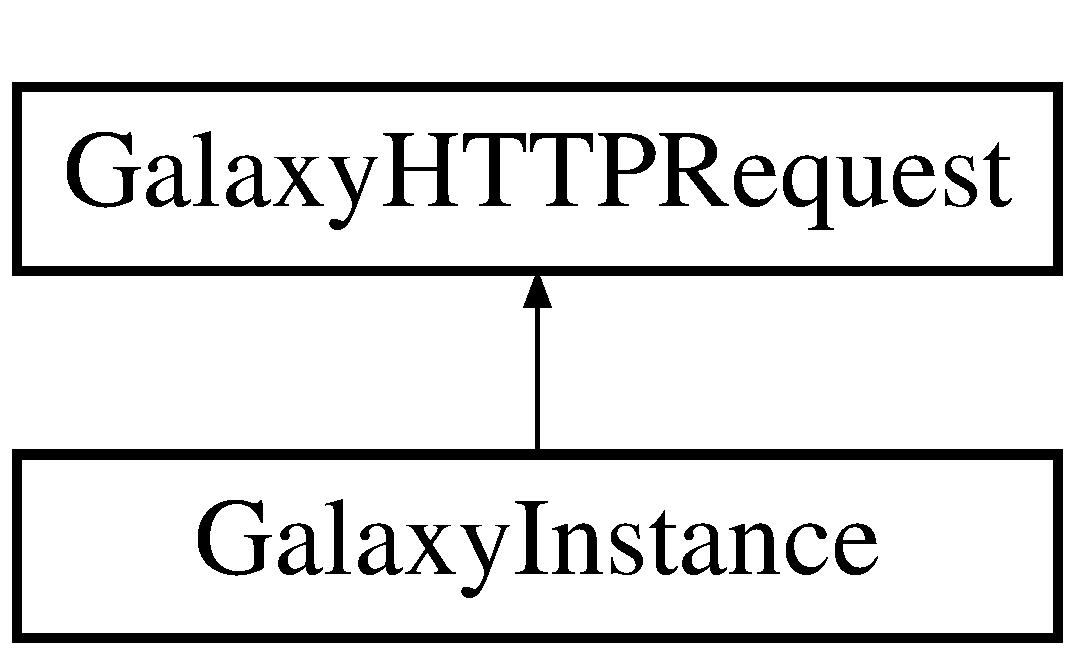
\includegraphics[height=2.000000cm]{classGalaxyHTTPRequest}
\end{center}
\end{figure}
\subsection*{Public Member Functions}
\begin{DoxyCompactItemize}
\item 
\hyperlink{classGalaxyHTTPRequest_acfb5537e004575571ac98724acb98aa1}{\-\_\-\-\_\-construct} ()
\item 
\hyperlink{classGalaxyHTTPRequest_aa158a65aa16bce21704f96f0a1b26a6b}{http\-G\-E\-T} (\$U\-R\-L, \$curl\-\_\-options=array())
\item 
\hyperlink{classGalaxyHTTPRequest_a3baf3c23d62fc0f7fd51198129a92819}{http\-P\-O\-S\-T} (\$U\-R\-L, \$input=N\-U\-L\-L)
\item 
\hyperlink{classGalaxyHTTPRequest_a54f7ae8f69da344ad0683657eba7b90e}{http\-P\-U\-T} (\$U\-R\-L, \$input=N\-U\-L\-L)
\item 
\hyperlink{classGalaxyHTTPRequest_a884e1813a5b594aa052ee9d44b4e9127}{http\-P\-A\-T\-C\-H} (\$U\-R\-L, \$input=N\-U\-L\-L)
\item 
\hyperlink{classGalaxyHTTPRequest_a522c94d27f40e84e11bf0020753d9d67}{get\-Remote\-File} (\$U\-R\-L, \$file\-\_\-name)
\item 
\hyperlink{classGalaxyHTTPRequest_a1b0ac0853de2c399956b6a64bb82b5ad}{upload\-File} (\$U\-R\-L, \$data, \$files)
\item 
\hyperlink{classGalaxyHTTPRequest_ac56712bb4a3c5437dbc581cba699198b}{http\-D\-E\-L\-E\-T\-E} (\$U\-R\-L, \$input=N\-U\-L\-L)
\item 
\hyperlink{classGalaxyHTTPRequest_a9e802c258f537b505aa18a3aec1315ba}{auth} (\$U\-R\-L, \$username, \$password)
\item 
\hyperlink{classGalaxyHTTPRequest_a72f394afb282f6e578ed12fd26a3d22f}{get\-Error} ()
\item 
\hyperlink{classGalaxyHTTPRequest_ac66ae869af44fe97917c6301329b23d4}{get\-Error\-Message} ()
\item 
\hyperlink{classGalaxyHTTPRequest_afb2ca4429dcaaa34246755ebdedcd7e7}{get\-Error\-Type} ()
\item 
\hyperlink{classGalaxyHTTPRequest_aa292af44a7986f5320510db8b2af3ae3}{set\-Error} (\$type, \$message)
\item 
\hyperlink{classGalaxyHTTPRequest_aed346abf2949176de07ee0db1a8de506}{expect\-Array} (\$response)
\end{DoxyCompactItemize}


\subsection{Constructor \& Destructor Documentation}
\hypertarget{classGalaxyHTTPRequest_acfb5537e004575571ac98724acb98aa1}{\index{Galaxy\-H\-T\-T\-P\-Request@{Galaxy\-H\-T\-T\-P\-Request}!\-\_\-\-\_\-construct@{\-\_\-\-\_\-construct}}
\index{\-\_\-\-\_\-construct@{\-\_\-\-\_\-construct}!GalaxyHTTPRequest@{Galaxy\-H\-T\-T\-P\-Request}}
\subsubsection[{\-\_\-\-\_\-construct}]{\setlength{\rightskip}{0pt plus 5cm}Galaxy\-H\-T\-T\-P\-Request\-::\-\_\-\-\_\-construct (
\begin{DoxyParamCaption}
{}
\end{DoxyParamCaption}
)}}\label{classGalaxyHTTPRequest_acfb5537e004575571ac98724acb98aa1}
The \hyperlink{classGalaxyHTTPRequest}{Galaxy\-H\-T\-T\-P\-Request} constructor.

\begin{DoxyReturn}{Returns}
An instance of a \hyperlink{classGalaxyHTTPRequest}{Galaxy\-H\-T\-T\-P\-Request} class. 
\end{DoxyReturn}


\subsection{Member Function Documentation}
\hypertarget{classGalaxyHTTPRequest_a9e802c258f537b505aa18a3aec1315ba}{\index{Galaxy\-H\-T\-T\-P\-Request@{Galaxy\-H\-T\-T\-P\-Request}!auth@{auth}}
\index{auth@{auth}!GalaxyHTTPRequest@{Galaxy\-H\-T\-T\-P\-Request}}
\subsubsection[{auth}]{\setlength{\rightskip}{0pt plus 5cm}Galaxy\-H\-T\-T\-P\-Request\-::auth (
\begin{DoxyParamCaption}
\item[{}]{\$\-U\-R\-L, }
\item[{}]{\$username, }
\item[{}]{\$password}
\end{DoxyParamCaption}
)}}\label{classGalaxyHTTPRequest_a9e802c258f537b505aa18a3aec1315ba}

\begin{DoxyParams}[1]{Parameters}
unknown & {\em \$\-U\-R\-L} & \\
\hline
unknown & {\em \$username} & \\
\hline
unknown & {\em \$password} & \\
\hline
\end{DoxyParams}
\hypertarget{classGalaxyHTTPRequest_aed346abf2949176de07ee0db1a8de506}{\index{Galaxy\-H\-T\-T\-P\-Request@{Galaxy\-H\-T\-T\-P\-Request}!expect\-Array@{expect\-Array}}
\index{expect\-Array@{expect\-Array}!GalaxyHTTPRequest@{Galaxy\-H\-T\-T\-P\-Request}}
\subsubsection[{expect\-Array}]{\setlength{\rightskip}{0pt plus 5cm}Galaxy\-H\-T\-T\-P\-Request\-::expect\-Array (
\begin{DoxyParamCaption}
\item[{}]{\$response}
\end{DoxyParamCaption}
)}}\label{classGalaxyHTTPRequest_aed346abf2949176de07ee0db1a8de506}
Checks if the provided value is an array and sets an error if not.

This is a helper function to help children class deal with the case when Galaxy does not return a J\-S\-O\-N array as expected. Sometimes when there is an error the error message is returned in a J\-S\-O\-N array and can be handled by our get\-C\-U\-R\-L\-Response function. But otherwise that function can't distinguish between a string that is returned and an error. So, this function allows children class to check that the response is an array if they expect that it should be.


\begin{DoxyParams}{Parameters}
{\em \$response} & \\
\hline
\end{DoxyParams}
\hypertarget{classGalaxyHTTPRequest_a72f394afb282f6e578ed12fd26a3d22f}{\index{Galaxy\-H\-T\-T\-P\-Request@{Galaxy\-H\-T\-T\-P\-Request}!get\-Error@{get\-Error}}
\index{get\-Error@{get\-Error}!GalaxyHTTPRequest@{Galaxy\-H\-T\-T\-P\-Request}}
\subsubsection[{get\-Error}]{\setlength{\rightskip}{0pt plus 5cm}Galaxy\-H\-T\-T\-P\-Request\-::get\-Error (
\begin{DoxyParamCaption}
{}
\end{DoxyParamCaption}
)}}\label{classGalaxyHTTPRequest_a72f394afb282f6e578ed12fd26a3d22f}
A wrapper function for retrieving an error.

Interacts with the \hyperlink{classGalaxyError}{Galaxy\-Error} object which is a private member of this class.

\begin{DoxySeeAlso}{See Also}
\hyperlink{classGalaxyError_a028ee131e1f68da22c29e510b405e0a7}{Galaxy\-Error\-::get\-Error()} 
\end{DoxySeeAlso}
\hypertarget{classGalaxyHTTPRequest_ac66ae869af44fe97917c6301329b23d4}{\index{Galaxy\-H\-T\-T\-P\-Request@{Galaxy\-H\-T\-T\-P\-Request}!get\-Error\-Message@{get\-Error\-Message}}
\index{get\-Error\-Message@{get\-Error\-Message}!GalaxyHTTPRequest@{Galaxy\-H\-T\-T\-P\-Request}}
\subsubsection[{get\-Error\-Message}]{\setlength{\rightskip}{0pt plus 5cm}Galaxy\-H\-T\-T\-P\-Request\-::get\-Error\-Message (
\begin{DoxyParamCaption}
{}
\end{DoxyParamCaption}
)}}\label{classGalaxyHTTPRequest_ac66ae869af44fe97917c6301329b23d4}
A wrapper function for retrieving an error message.

Interacts with the \hyperlink{classGalaxyError}{Galaxy\-Error} object which is a private member of this class.

\begin{DoxySeeAlso}{See Also}
\hyperlink{classGalaxyError_a1f1ec54a9bcb9520dbaa7abc3e163824}{Galaxy\-Error\-::get\-Error\-Message()} 
\end{DoxySeeAlso}
\hypertarget{classGalaxyHTTPRequest_afb2ca4429dcaaa34246755ebdedcd7e7}{\index{Galaxy\-H\-T\-T\-P\-Request@{Galaxy\-H\-T\-T\-P\-Request}!get\-Error\-Type@{get\-Error\-Type}}
\index{get\-Error\-Type@{get\-Error\-Type}!GalaxyHTTPRequest@{Galaxy\-H\-T\-T\-P\-Request}}
\subsubsection[{get\-Error\-Type}]{\setlength{\rightskip}{0pt plus 5cm}Galaxy\-H\-T\-T\-P\-Request\-::get\-Error\-Type (
\begin{DoxyParamCaption}
{}
\end{DoxyParamCaption}
)}}\label{classGalaxyHTTPRequest_afb2ca4429dcaaa34246755ebdedcd7e7}
A wrapper function for retrieving an error type.

Interacts with the \hyperlink{classGalaxyError}{Galaxy\-Error} object which is a private member of this class.

\begin{DoxySeeAlso}{See Also}
\hyperlink{classGalaxyError_a2e680e1a6475af8dfbcb6d1f07254f8c}{Galaxy\-Error\-::get\-Error\-Type()} 
\end{DoxySeeAlso}
\hypertarget{classGalaxyHTTPRequest_a522c94d27f40e84e11bf0020753d9d67}{\index{Galaxy\-H\-T\-T\-P\-Request@{Galaxy\-H\-T\-T\-P\-Request}!get\-Remote\-File@{get\-Remote\-File}}
\index{get\-Remote\-File@{get\-Remote\-File}!GalaxyHTTPRequest@{Galaxy\-H\-T\-T\-P\-Request}}
\subsubsection[{get\-Remote\-File}]{\setlength{\rightskip}{0pt plus 5cm}Galaxy\-H\-T\-T\-P\-Request\-::get\-Remote\-File (
\begin{DoxyParamCaption}
\item[{}]{\$\-U\-R\-L, }
\item[{}]{\$file\-\_\-name}
\end{DoxyParamCaption}
)}}\label{classGalaxyHTTPRequest_a522c94d27f40e84e11bf0020753d9d67}

\begin{DoxyParams}{Parameters}
{\em \$\-U\-R\-L} & \\
\hline
{\em \$file\-\_\-name} & \\
\hline
\end{DoxyParams}
\begin{DoxyReturn}{Returns}

\end{DoxyReturn}
\hypertarget{classGalaxyHTTPRequest_ac56712bb4a3c5437dbc581cba699198b}{\index{Galaxy\-H\-T\-T\-P\-Request@{Galaxy\-H\-T\-T\-P\-Request}!http\-D\-E\-L\-E\-T\-E@{http\-D\-E\-L\-E\-T\-E}}
\index{http\-D\-E\-L\-E\-T\-E@{http\-D\-E\-L\-E\-T\-E}!GalaxyHTTPRequest@{Galaxy\-H\-T\-T\-P\-Request}}
\subsubsection[{http\-D\-E\-L\-E\-T\-E}]{\setlength{\rightskip}{0pt plus 5cm}Galaxy\-H\-T\-T\-P\-Request\-::http\-D\-E\-L\-E\-T\-E (
\begin{DoxyParamCaption}
\item[{}]{\$\-U\-R\-L, }
\item[{}]{\$input = {\ttfamily NULL}}
\end{DoxyParamCaption}
)}}\label{classGalaxyHTTPRequest_ac56712bb4a3c5437dbc581cba699198b}
Universal D\-E\-L\-E\-T\-E request


\begin{DoxyParams}{Parameters}
{\em \$input} & The input data to give to the url. \\
\hline
{\em \$\-U\-R\-L} & The path to perform the D\-E\-L\-E\-T\-E request.\\
\hline
\end{DoxyParams}
\begin{DoxyReturn}{Returns}
curl server response 
\end{DoxyReturn}
\hypertarget{classGalaxyHTTPRequest_aa158a65aa16bce21704f96f0a1b26a6b}{\index{Galaxy\-H\-T\-T\-P\-Request@{Galaxy\-H\-T\-T\-P\-Request}!http\-G\-E\-T@{http\-G\-E\-T}}
\index{http\-G\-E\-T@{http\-G\-E\-T}!GalaxyHTTPRequest@{Galaxy\-H\-T\-T\-P\-Request}}
\subsubsection[{http\-G\-E\-T}]{\setlength{\rightskip}{0pt plus 5cm}Galaxy\-H\-T\-T\-P\-Request\-::http\-G\-E\-T (
\begin{DoxyParamCaption}
\item[{}]{\$\-U\-R\-L, }
\item[{}]{\$curl\-\_\-options = {\ttfamily array()}}
\end{DoxyParamCaption}
)}}\label{classGalaxyHTTPRequest_aa158a65aa16bce21704f96f0a1b26a6b}
Performs a G\-E\-T request.


\begin{DoxyParams}{Parameters}
{\em \$\-U\-R\-L} & The U\-R\-L for the G\-E\-T. \\
\hline
{\em \$curl\-\_\-options} & Any additional information to retreive from the resource while the G\-E\-T request...yo. \\
\hline
\end{DoxyParams}
\begin{DoxyReturn}{Returns}
curl server response. 
\end{DoxyReturn}
\hypertarget{classGalaxyHTTPRequest_a884e1813a5b594aa052ee9d44b4e9127}{\index{Galaxy\-H\-T\-T\-P\-Request@{Galaxy\-H\-T\-T\-P\-Request}!http\-P\-A\-T\-C\-H@{http\-P\-A\-T\-C\-H}}
\index{http\-P\-A\-T\-C\-H@{http\-P\-A\-T\-C\-H}!GalaxyHTTPRequest@{Galaxy\-H\-T\-T\-P\-Request}}
\subsubsection[{http\-P\-A\-T\-C\-H}]{\setlength{\rightskip}{0pt plus 5cm}Galaxy\-H\-T\-T\-P\-Request\-::http\-P\-A\-T\-C\-H (
\begin{DoxyParamCaption}
\item[{}]{\$\-U\-R\-L, }
\item[{}]{\$input = {\ttfamily NULL}}
\end{DoxyParamCaption}
)}}\label{classGalaxyHTTPRequest_a884e1813a5b594aa052ee9d44b4e9127}
Perform a P\-A\-T\-C\-H request


\begin{DoxyParams}{Parameters}
{\em \$\-U\-R\-L} & The U\-R\-L for the P\-A\-T\-C\-H request.\\
\hline
{\em \$input} & The input data to give to the U\-R\-L.\\
\hline
\end{DoxyParams}
\begin{DoxyReturn}{Returns}
curl server response. 
\end{DoxyReturn}
\hypertarget{classGalaxyHTTPRequest_a3baf3c23d62fc0f7fd51198129a92819}{\index{Galaxy\-H\-T\-T\-P\-Request@{Galaxy\-H\-T\-T\-P\-Request}!http\-P\-O\-S\-T@{http\-P\-O\-S\-T}}
\index{http\-P\-O\-S\-T@{http\-P\-O\-S\-T}!GalaxyHTTPRequest@{Galaxy\-H\-T\-T\-P\-Request}}
\subsubsection[{http\-P\-O\-S\-T}]{\setlength{\rightskip}{0pt plus 5cm}Galaxy\-H\-T\-T\-P\-Request\-::http\-P\-O\-S\-T (
\begin{DoxyParamCaption}
\item[{}]{\$\-U\-R\-L, }
\item[{}]{\$input = {\ttfamily NULL}}
\end{DoxyParamCaption}
)}}\label{classGalaxyHTTPRequest_a3baf3c23d62fc0f7fd51198129a92819}
Perform a P\-O\-S\-T request.


\begin{DoxyParams}{Parameters}
{\em \$\-U\-R\-L} & The url for the P\-O\-S\-T. \\
\hline
{\em \$input} & The input data to a given U\-R\-L.\\
\hline
\end{DoxyParams}
\begin{DoxyReturn}{Returns}
curl server response. 
\end{DoxyReturn}
\hypertarget{classGalaxyHTTPRequest_a54f7ae8f69da344ad0683657eba7b90e}{\index{Galaxy\-H\-T\-T\-P\-Request@{Galaxy\-H\-T\-T\-P\-Request}!http\-P\-U\-T@{http\-P\-U\-T}}
\index{http\-P\-U\-T@{http\-P\-U\-T}!GalaxyHTTPRequest@{Galaxy\-H\-T\-T\-P\-Request}}
\subsubsection[{http\-P\-U\-T}]{\setlength{\rightskip}{0pt plus 5cm}Galaxy\-H\-T\-T\-P\-Request\-::http\-P\-U\-T (
\begin{DoxyParamCaption}
\item[{}]{\$\-U\-R\-L, }
\item[{}]{\$input = {\ttfamily NULL}}
\end{DoxyParamCaption}
)}}\label{classGalaxyHTTPRequest_a54f7ae8f69da344ad0683657eba7b90e}
Perform a P\-U\-T request


\begin{DoxyParams}{Parameters}
{\em \$\-U\-R\-L} & The U\-R\-L for the P\-U\-T\\
\hline
{\em \$input} & The input data to give to the U\-R\-L.\\
\hline
\end{DoxyParams}
\begin{DoxyReturn}{Returns}
An associative array containing the response from the Galaxy server or F\-A\-L\-S\-E if an error occured. If F\-A\-L\-S\-E then use the \hyperlink{classGalaxyHTTPRequest_a72f394afb282f6e578ed12fd26a3d22f}{get\-Error()} function to retrieve the error message and type. 
\end{DoxyReturn}
\hypertarget{classGalaxyHTTPRequest_aa292af44a7986f5320510db8b2af3ae3}{\index{Galaxy\-H\-T\-T\-P\-Request@{Galaxy\-H\-T\-T\-P\-Request}!set\-Error@{set\-Error}}
\index{set\-Error@{set\-Error}!GalaxyHTTPRequest@{Galaxy\-H\-T\-T\-P\-Request}}
\subsubsection[{set\-Error}]{\setlength{\rightskip}{0pt plus 5cm}Galaxy\-H\-T\-T\-P\-Request\-::set\-Error (
\begin{DoxyParamCaption}
\item[{}]{\$type, }
\item[{}]{\$message}
\end{DoxyParamCaption}
)}}\label{classGalaxyHTTPRequest_aa292af44a7986f5320510db8b2af3ae3}
A wrapper function for setting an error.

Interacts with the \hyperlink{classGalaxyError}{Galaxy\-Error} object which is a private member of this class.

\begin{DoxySeeAlso}{See Also}
\hyperlink{classGalaxyError_a4c3312a17a9f150a6a64b44b345a6143}{Galaxy\-Error\-::set\-Error()} 
\end{DoxySeeAlso}
\hypertarget{classGalaxyHTTPRequest_a1b0ac0853de2c399956b6a64bb82b5ad}{\index{Galaxy\-H\-T\-T\-P\-Request@{Galaxy\-H\-T\-T\-P\-Request}!upload\-File@{upload\-File}}
\index{upload\-File@{upload\-File}!GalaxyHTTPRequest@{Galaxy\-H\-T\-T\-P\-Request}}
\subsubsection[{upload\-File}]{\setlength{\rightskip}{0pt plus 5cm}Galaxy\-H\-T\-T\-P\-Request\-::upload\-File (
\begin{DoxyParamCaption}
\item[{}]{\$\-U\-R\-L, }
\item[{}]{\$data, }
\item[{}]{\$files}
\end{DoxyParamCaption}
)}}\label{classGalaxyHTTPRequest_a1b0ac0853de2c399956b6a64bb82b5ad}
Upload file request


\begin{DoxyParams}{Parameters}
{\em \$data} & The input data to give to the url. \\
\hline
{\em \$\-U\-R\-L} & The path to perform the D\-E\-L\-E\-T\-E request. \\
\hline
{\em \$files} & The file(s) to post to the specified U\-R\-L\\
\hline
\end{DoxyParams}
\begin{DoxyReturn}{Returns}
curl server response 
\end{DoxyReturn}


The documentation for this class was generated from the following file\-:\begin{DoxyCompactItemize}
\item 
H\-T\-T\-P\-Request.\-inc\end{DoxyCompactItemize}

\hypertarget{classGalaxyInstance}{\section{Galaxy\-Instance Class Reference}
\label{classGalaxyInstance}\index{Galaxy\-Instance@{Galaxy\-Instance}}
}
Inheritance diagram for Galaxy\-Instance\-:\begin{figure}[H]
\begin{center}
\leavevmode
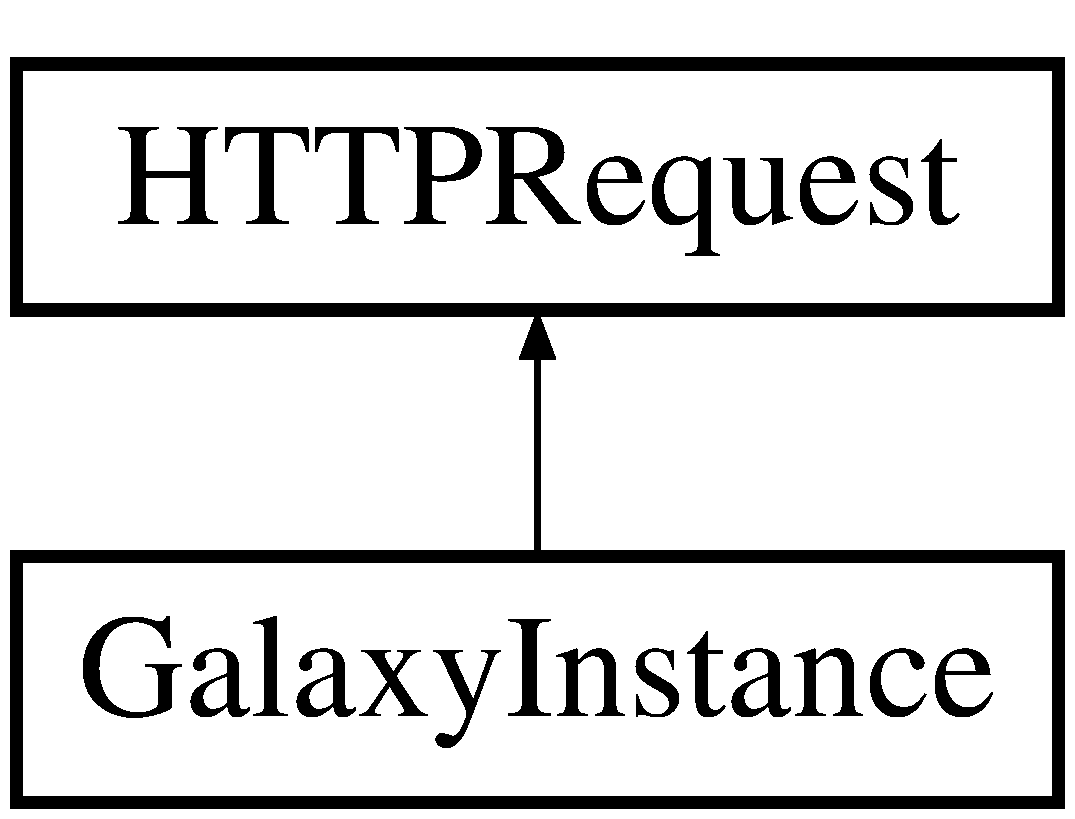
\includegraphics[height=2.000000cm]{classGalaxyInstance}
\end{center}
\end{figure}
\subsection*{Public Member Functions}
\begin{DoxyCompactItemize}
\item 
\hyperlink{classGalaxyInstance_a98d1b5f750ce3be53e96e435917b63b1}{\-\_\-\-\_\-construct} (\$hostname, \$port, \$use\-\_\-https=F\-A\-L\-S\-E)
\item 
\hyperlink{classGalaxyInstance_afbb7256306223f7f8ee85f85868e2de2}{get\-Version} ()
\item 
\hyperlink{classGalaxyInstance_a243315a49fd4ba0df8916b87872299ed}{authenticate} (\$username, \$password, \&\$message= '')
\item 
\hyperlink{classGalaxyInstance_a5b0c7191b82c21d857ec3d42068f3cf4}{get\-U\-R\-L} ()
\item 
\hyperlink{classGalaxyInstance_a4e4c854e91c21917adebec78a655edd3}{set\-A\-P\-I\-Key} (\$api\-\_\-key)
\item 
\hyperlink{classGalaxyInstance_a563deeb4f829462d7476d3684ed099cb}{get\-A\-P\-I\-Key} ()
\end{DoxyCompactItemize}
\subsection*{Protected Attributes}
\begin{DoxyCompactItemize}
\item 
\hyperlink{classGalaxyInstance_a68aaf747e0eae3b9338cd4c51711b514}{\$host}
\item 
\hyperlink{classGalaxyInstance_ab70c08b0781f835e1a2e4388b1baa639}{\$port}
\item 
\hyperlink{classGalaxyInstance_ab920cbfc8f2f63f3793ba067ee523ca8}{\$use\-\_\-https}
\item 
\hyperlink{classGalaxyInstance_a2a67b0838ca6175e9e01e3045b666caf}{\$api\-\_\-key}
\end{DoxyCompactItemize}


\subsection{Constructor \& Destructor Documentation}
\hypertarget{classGalaxyInstance_a98d1b5f750ce3be53e96e435917b63b1}{\index{Galaxy\-Instance@{Galaxy\-Instance}!\-\_\-\-\_\-construct@{\-\_\-\-\_\-construct}}
\index{\-\_\-\-\_\-construct@{\-\_\-\-\_\-construct}!GalaxyInstance@{Galaxy\-Instance}}
\subsubsection[{\-\_\-\-\_\-construct}]{\setlength{\rightskip}{0pt plus 5cm}Galaxy\-Instance\-::\-\_\-\-\_\-construct (
\begin{DoxyParamCaption}
\item[{}]{\$hostname, }
\item[{}]{\$port, }
\item[{}]{\$use\-\_\-https = {\ttfamily FALSE}}
\end{DoxyParamCaption}
)}}\label{classGalaxyInstance_a98d1b5f750ce3be53e96e435917b63b1}
The \hyperlink{classGalaxyInstance}{Galaxy\-Instance} constructor.


\begin{DoxyParams}{Parameters}
{\em \$hostname} & The hostname where the Galaxy server is located. \\
\hline
{\em \$port} & The port on which the remote Galaxy instance is runinng. \\
\hline
{\em \$use\-\_\-https} & Should be set to T\-R\-U\-E if the remote server uses H\-T\-T\-P\-S. Defaults to T\-R\-U\-E.\\
\hline
\end{DoxyParams}
\begin{DoxyReturn}{Returns}
An instance of a \hyperlink{classGalaxyInstance}{Galaxy\-Instance} object. 
\end{DoxyReturn}


\subsection{Member Function Documentation}
\hypertarget{classGalaxyInstance_a243315a49fd4ba0df8916b87872299ed}{\index{Galaxy\-Instance@{Galaxy\-Instance}!authenticate@{authenticate}}
\index{authenticate@{authenticate}!GalaxyInstance@{Galaxy\-Instance}}
\subsubsection[{authenticate}]{\setlength{\rightskip}{0pt plus 5cm}Galaxy\-Instance\-::authenticate (
\begin{DoxyParamCaption}
\item[{}]{\$username, }
\item[{}]{\$password, }
\item[{\&}]{\$message = {\ttfamily ''}}
\end{DoxyParamCaption}
)}}\label{classGalaxyInstance_a243315a49fd4ba0df8916b87872299ed}
Authenticates a user with the remote Galaxy instance.

Corresponds to the Galaxy A\-P\-I method and path\-: G\-E\-T /api/authenticate/baseauth


\begin{DoxyParams}{Parameters}
{\em \$username} & The username of the user. \\
\hline
{\em \$password} & The password for the user. \\
\hline
{\em \$message} & If authentication fails then this variable will be set to contain the error message.\\
\hline
\end{DoxyParams}
\begin{DoxyReturn}{Returns}
T\-R\-U\-E if authentication was successful, F\-A\-L\-S\-E otherwise. 
\end{DoxyReturn}
\hypertarget{classGalaxyInstance_a563deeb4f829462d7476d3684ed099cb}{\index{Galaxy\-Instance@{Galaxy\-Instance}!get\-A\-P\-I\-Key@{get\-A\-P\-I\-Key}}
\index{get\-A\-P\-I\-Key@{get\-A\-P\-I\-Key}!GalaxyInstance@{Galaxy\-Instance}}
\subsubsection[{get\-A\-P\-I\-Key}]{\setlength{\rightskip}{0pt plus 5cm}Galaxy\-Instance\-::get\-A\-P\-I\-Key (
\begin{DoxyParamCaption}
{}
\end{DoxyParamCaption}
)}}\label{classGalaxyInstance_a563deeb4f829462d7476d3684ed099cb}
Acquires the A\-P\-I key

\begin{DoxyReturn}{Returns}
string The A\-P\-I key that authorizes a user to certain actions. 
\end{DoxyReturn}
\hypertarget{classGalaxyInstance_a5b0c7191b82c21d857ec3d42068f3cf4}{\index{Galaxy\-Instance@{Galaxy\-Instance}!get\-U\-R\-L@{get\-U\-R\-L}}
\index{get\-U\-R\-L@{get\-U\-R\-L}!GalaxyInstance@{Galaxy\-Instance}}
\subsubsection[{get\-U\-R\-L}]{\setlength{\rightskip}{0pt plus 5cm}Galaxy\-Instance\-::get\-U\-R\-L (
\begin{DoxyParamCaption}
{}
\end{DoxyParamCaption}
)}}\label{classGalaxyInstance_a5b0c7191b82c21d857ec3d42068f3cf4}
Returns the U\-R\-L for the remote Galaxy server.

The U\-R\-L returned will include the protocol (H\-T\-T\-P, H\-T\-T\-P\-S), the hostname and the port.

\begin{DoxyReturn}{Returns}
string The U\-R\-L for the remote Galaxy instance. 
\end{DoxyReturn}
\hypertarget{classGalaxyInstance_afbb7256306223f7f8ee85f85868e2de2}{\index{Galaxy\-Instance@{Galaxy\-Instance}!get\-Version@{get\-Version}}
\index{get\-Version@{get\-Version}!GalaxyInstance@{Galaxy\-Instance}}
\subsubsection[{get\-Version}]{\setlength{\rightskip}{0pt plus 5cm}Galaxy\-Instance\-::get\-Version (
\begin{DoxyParamCaption}
{}
\end{DoxyParamCaption}
)}}\label{classGalaxyInstance_afbb7256306223f7f8ee85f85868e2de2}
Retrieves the version of the Galaxy A\-P\-I.

\begin{DoxyReturn}{Returns}

\end{DoxyReturn}
\hypertarget{classGalaxyInstance_a4e4c854e91c21917adebec78a655edd3}{\index{Galaxy\-Instance@{Galaxy\-Instance}!set\-A\-P\-I\-Key@{set\-A\-P\-I\-Key}}
\index{set\-A\-P\-I\-Key@{set\-A\-P\-I\-Key}!GalaxyInstance@{Galaxy\-Instance}}
\subsubsection[{set\-A\-P\-I\-Key}]{\setlength{\rightskip}{0pt plus 5cm}Galaxy\-Instance\-::set\-A\-P\-I\-Key (
\begin{DoxyParamCaption}
\item[{}]{\$api\-\_\-key}
\end{DoxyParamCaption}
)}}\label{classGalaxyInstance_a4e4c854e91c21917adebec78a655edd3}
Sets the A\-P\-I Key for this Galaxy instance.


\begin{DoxyParams}{Parameters}
{\em \$api\-\_\-key} & The A\-P\-I key of the Galaxy user. \\
\hline
\end{DoxyParams}


\subsection{Member Data Documentation}
\hypertarget{classGalaxyInstance_a2a67b0838ca6175e9e01e3045b666caf}{\index{Galaxy\-Instance@{Galaxy\-Instance}!\$api\-\_\-key@{\$api\-\_\-key}}
\index{\$api\-\_\-key@{\$api\-\_\-key}!GalaxyInstance@{Galaxy\-Instance}}
\subsubsection[{\$api\-\_\-key}]{\setlength{\rightskip}{0pt plus 5cm}Galaxy\-Instance\-::\$api\-\_\-key\hspace{0.3cm}{\ttfamily [protected]}}}\label{classGalaxyInstance_a2a67b0838ca6175e9e01e3045b666caf}
The A\-P\-I Key for the user connection. \hypertarget{classGalaxyInstance_a68aaf747e0eae3b9338cd4c51711b514}{\index{Galaxy\-Instance@{Galaxy\-Instance}!\$host@{\$host}}
\index{\$host@{\$host}!GalaxyInstance@{Galaxy\-Instance}}
\subsubsection[{\$host}]{\setlength{\rightskip}{0pt plus 5cm}Galaxy\-Instance\-::\$host\hspace{0.3cm}{\ttfamily [protected]}}}\label{classGalaxyInstance_a68aaf747e0eae3b9338cd4c51711b514}
The hostname where the Galaxy server is located. \hypertarget{classGalaxyInstance_ab70c08b0781f835e1a2e4388b1baa639}{\index{Galaxy\-Instance@{Galaxy\-Instance}!\$port@{\$port}}
\index{\$port@{\$port}!GalaxyInstance@{Galaxy\-Instance}}
\subsubsection[{\$port}]{\setlength{\rightskip}{0pt plus 5cm}Galaxy\-Instance\-::\$port\hspace{0.3cm}{\ttfamily [protected]}}}\label{classGalaxyInstance_ab70c08b0781f835e1a2e4388b1baa639}
The port on which the remote Galaxy instance is runinng. \hypertarget{classGalaxyInstance_ab920cbfc8f2f63f3793ba067ee523ca8}{\index{Galaxy\-Instance@{Galaxy\-Instance}!\$use\-\_\-https@{\$use\-\_\-https}}
\index{\$use\-\_\-https@{\$use\-\_\-https}!GalaxyInstance@{Galaxy\-Instance}}
\subsubsection[{\$use\-\_\-https}]{\setlength{\rightskip}{0pt plus 5cm}Galaxy\-Instance\-::\$use\-\_\-https\hspace{0.3cm}{\ttfamily [protected]}}}\label{classGalaxyInstance_ab920cbfc8f2f63f3793ba067ee523ca8}
Should be set to T\-R\-U\-E if the remote server uses H\-T\-T\-P\-S. 

The documentation for this class was generated from the following file\-:\begin{DoxyCompactItemize}
\item 
Galaxy\-Instance.\-inc\end{DoxyCompactItemize}

\hypertarget{classGalaxyJobs}{\section{Galaxy\-Jobs Class Reference}
\label{classGalaxyJobs}\index{Galaxy\-Jobs@{Galaxy\-Jobs}}
}
\subsection*{Public Member Functions}
\begin{DoxyCompactItemize}
\item 
\hyperlink{classGalaxyJobs_a303bce11eaaf0a7493920b16bce8a704}{\-\_\-\-\_\-construct} (\hyperlink{classGalaxyInstance}{Galaxy\-Instance} \$galaxy)
\item 
\hyperlink{classGalaxyJobs_a583ac2bfe50692c1332d79641aebc288}{build\-For\-Rerun} (\$params)
\item 
\hyperlink{classGalaxyJobs_a489e7e3595e44cecc3f6cfb8b2b7353f}{inputs} (\$params)
\item 
\hyperlink{classGalaxyJobs_a2e33c69ed69aabf03fd73c8671aacd88}{outputs} (\$params)
\item 
\hyperlink{classGalaxyJobs_a0e1e071fe034d943cd9e5f6301d01c11}{show} (\$params)
\item 
\hyperlink{classGalaxyJobs_a9472246111b1011169a0900320162fc8}{index} (\$params)
\item 
\hyperlink{classGalaxyJobs_acdef8cbf37424947838dee85ebe86e21}{create} ()
\item 
\hyperlink{classGalaxyJobs_aced9ee757a9e61e861c9198102639cbc}{search} (\$params)
\end{DoxyCompactItemize}


\subsection{Constructor \& Destructor Documentation}
\hypertarget{classGalaxyJobs_a303bce11eaaf0a7493920b16bce8a704}{\index{Galaxy\-Jobs@{Galaxy\-Jobs}!\-\_\-\-\_\-construct@{\-\_\-\-\_\-construct}}
\index{\-\_\-\-\_\-construct@{\-\_\-\-\_\-construct}!GalaxyJobs@{Galaxy\-Jobs}}
\subsubsection[{\-\_\-\-\_\-construct}]{\setlength{\rightskip}{0pt plus 5cm}Galaxy\-Jobs\-::\-\_\-\-\_\-construct (
\begin{DoxyParamCaption}
\item[{{\bf Galaxy\-Instance}}]{\$galaxy}
\end{DoxyParamCaption}
)}}\label{classGalaxyJobs_a303bce11eaaf0a7493920b16bce8a704}
The Jobs constructor.


\begin{DoxyParams}[1]{Parameters}
\hyperlink{classGalaxyInstance}{Galaxy\-Instance} & {\em \$galaxy} & A \hyperlink{classGalaxyInstance}{Galaxy\-Instance} object.\\
\hline
\end{DoxyParams}
\begin{DoxyReturn}{Returns}
An instance of a Jobs object. 
\end{DoxyReturn}


\subsection{Member Function Documentation}
\hypertarget{classGalaxyJobs_a583ac2bfe50692c1332d79641aebc288}{\index{Galaxy\-Jobs@{Galaxy\-Jobs}!build\-For\-Rerun@{build\-For\-Rerun}}
\index{build\-For\-Rerun@{build\-For\-Rerun}!GalaxyJobs@{Galaxy\-Jobs}}
\subsubsection[{build\-For\-Rerun}]{\setlength{\rightskip}{0pt plus 5cm}Galaxy\-Jobs\-::build\-For\-Rerun (
\begin{DoxyParamCaption}
\item[{}]{\$params}
\end{DoxyParamCaption}
)}}\label{classGalaxyJobs_a583ac2bfe50692c1332d79641aebc288}
Retreive a tool input template populated with this job's information.

Corresponds to the Galaxy Api/path at\-: G\-E\-T /api/jobs/\{encoded\-\_\-job\-\_\-id\}/build\-\_\-for\-\_\-rerun This function is suitable for rerunning or rendering parameters of the job.


\begin{DoxyParams}{Parameters}
{\em \$params} & An associative array containing the input parameters for this function. The following parameters are available\-:\\
\hline
\end{DoxyParams}

\begin{DoxyItemize}
\item id\-: The job id of the job whose information to retreive. The job id can be ontained from this class's \hyperlink{classGalaxyJobs_a9472246111b1011169a0900320162fc8}{index()} function.
\end{DoxyItemize}

\begin{DoxyReturn}{Returns}
An array containing ouput informaiton of the tool that has been built. 
\end{DoxyReturn}
\hypertarget{classGalaxyJobs_acdef8cbf37424947838dee85ebe86e21}{\index{Galaxy\-Jobs@{Galaxy\-Jobs}!create@{create}}
\index{create@{create}!GalaxyJobs@{Galaxy\-Jobs}}
\subsubsection[{create}]{\setlength{\rightskip}{0pt plus 5cm}Galaxy\-Jobs\-::create (
\begin{DoxyParamCaption}
{}
\end{DoxyParamCaption}
)}}\label{classGalaxyJobs_acdef8cbf37424947838dee85ebe86e21}
This function is not implemented by its python counterpart

N\-O\-T\-E\-: Creating/submitting a job is actually run under tools.\-py in the Galaxy api

\begin{DoxyReturn}{Returns}
F\-A\-L\-S\-E 
\end{DoxyReturn}
\hypertarget{classGalaxyJobs_a9472246111b1011169a0900320162fc8}{\index{Galaxy\-Jobs@{Galaxy\-Jobs}!index@{index}}
\index{index@{index}!GalaxyJobs@{Galaxy\-Jobs}}
\subsubsection[{index}]{\setlength{\rightskip}{0pt plus 5cm}Galaxy\-Jobs\-::index (
\begin{DoxyParamCaption}
\item[{}]{\$params}
\end{DoxyParamCaption}
)}}\label{classGalaxyJobs_a9472246111b1011169a0900320162fc8}
Retreive a list of jobs for current user.

Corresponds to the Galaxy Api method/path\-: G\-E\-T /api/jobs


\begin{DoxyParams}{Parameters}
{\em \$params} & An associative array containing the input parameters for this function. The following parameters are available\-:\\
\hline
\end{DoxyParams}

\begin{DoxyItemize}
\item state\-: filter job search by any one of these conditions\-: (i) 'new' (ii) 'upload' (iii) 'waiting' (iv) 'queued' (v) 'running' (vi) 'ok' (vii) 'error' (viii) 'paused' (ix) 'deleted' (x) 'deleted\-\_\-now'
\item tool\-\_\-ids\-: A list of tool ids that limit the search to include only those with given tool\-\_\-ids. To find tool id's, please refer to this class's \hyperlink{classGalaxyJobs_a9472246111b1011169a0900320162fc8}{index()} function.
\item date\-\_\-range\-\_\-min\-: Limit the search of jobs updated after this date.
\item date\-\_\-range\-\_\-max\-: Limit the search of jobs updated before this date.
\item history\-\_\-id\-: Limit listing of jobs to those that match history\-\_\-id. To find the history id, please refer to the history class.
\end{DoxyItemize}

\begin{DoxyReturn}{Returns}
An array containing a list of all the jobs that matched the given parameters. 
\end{DoxyReturn}
\hypertarget{classGalaxyJobs_a489e7e3595e44cecc3f6cfb8b2b7353f}{\index{Galaxy\-Jobs@{Galaxy\-Jobs}!inputs@{inputs}}
\index{inputs@{inputs}!GalaxyJobs@{Galaxy\-Jobs}}
\subsubsection[{inputs}]{\setlength{\rightskip}{0pt plus 5cm}Galaxy\-Jobs\-::inputs (
\begin{DoxyParamCaption}
\item[{}]{\$params}
\end{DoxyParamCaption}
)}}\label{classGalaxyJobs_a489e7e3595e44cecc3f6cfb8b2b7353f}
Retreive the input datasets created from the specified job.

Corresponds to the Galaxy Api/path at\-: G\-E\-T/api/jobs/\{encoded\-\_\-job\-\_\-id\}/inputs


\begin{DoxyParams}{Parameters}
{\em \$params} & An associative array containing the input parameters for this function. The following parameters are available\-:\\
\hline
\end{DoxyParams}

\begin{DoxyItemize}
\item job\-\_\-id\-: The job id of the job whose information to retreive. The job id can be ontained from this class's \hyperlink{classGalaxyJobs_a9472246111b1011169a0900320162fc8}{index()} function.
\end{DoxyItemize}

\begin{DoxyReturn}{Returns}
An array containing ouput informaiton of the job input. 
\end{DoxyReturn}
\hypertarget{classGalaxyJobs_a2e33c69ed69aabf03fd73c8671aacd88}{\index{Galaxy\-Jobs@{Galaxy\-Jobs}!outputs@{outputs}}
\index{outputs@{outputs}!GalaxyJobs@{Galaxy\-Jobs}}
\subsubsection[{outputs}]{\setlength{\rightskip}{0pt plus 5cm}Galaxy\-Jobs\-::outputs (
\begin{DoxyParamCaption}
\item[{}]{\$params}
\end{DoxyParamCaption}
)}}\label{classGalaxyJobs_a2e33c69ed69aabf03fd73c8671aacd88}
Retreive the output datasets created from the specified job.

Corresponds to the Galaxy Api/path at\-: G\-E\-T/api/jobs/\{encoded\-\_\-job\-\_\-id\}/inputs.


\begin{DoxyParams}{Parameters}
{\em \$params} & An associative array containing the input parameters for this function. The following parameters are available\-:\\
\hline
\end{DoxyParams}

\begin{DoxyItemize}
\item job\-\_\-id\-: The job id of the job whose information to retreive. The job id can be ontained from this class's \hyperlink{classGalaxyJobs_a9472246111b1011169a0900320162fc8}{index()} function.
\end{DoxyItemize}

\begin{DoxyReturn}{Returns}
An array containing ouput informaiton of the job outputs. 
\end{DoxyReturn}
\hypertarget{classGalaxyJobs_aced9ee757a9e61e861c9198102639cbc}{\index{Galaxy\-Jobs@{Galaxy\-Jobs}!search@{search}}
\index{search@{search}!GalaxyJobs@{Galaxy\-Jobs}}
\subsubsection[{search}]{\setlength{\rightskip}{0pt plus 5cm}Galaxy\-Jobs\-::search (
\begin{DoxyParamCaption}
\item[{}]{\$params}
\end{DoxyParamCaption}
)}}\label{classGalaxyJobs_aced9ee757a9e61e861c9198102639cbc}
Search for previously created jobs.

Corresponds to the Galaxy api/path at\-: P\-O\-S\-T /api/jobs/search

This method is designed to scan the list of previously run jobs and find records of jobs that had the exact some input parameters and datasets. This can be used to minimize, the amount of repeated work, and simplyrecycle the old results.


\begin{DoxyParams}{Parameters}
{\em \$params} & An associative array containing the input parameters for this function. The following parameters are available\-:\\
\hline
\end{DoxyParams}

\begin{DoxyItemize}
\item tool\-\_\-id\-: Required. The tool id to execute. To find the tool id, use the index function of this class.
\item inputs\-: Required. An associative array of key/value pairs where valid keys are 'id' and 'src' and 'id' is a tool\-\_\-id (e.\-g. wc\-\_\-gnu), and 'src' is is optional but defaults to 'hda'. Alternatively, if multiple inputs are desired, this can be an array of associative arrays.
\item state\-: Optional. The state of the job\-: 'running', 'queued', 'waiting', 'ok'. \begin{DoxyReturn}{Returns}
An array of jobs matching the provided arguments. 
\end{DoxyReturn}

\end{DoxyItemize}\hypertarget{classGalaxyJobs_a0e1e071fe034d943cd9e5f6301d01c11}{\index{Galaxy\-Jobs@{Galaxy\-Jobs}!show@{show}}
\index{show@{show}!GalaxyJobs@{Galaxy\-Jobs}}
\subsubsection[{show}]{\setlength{\rightskip}{0pt plus 5cm}Galaxy\-Jobs\-::show (
\begin{DoxyParamCaption}
\item[{}]{\$params}
\end{DoxyParamCaption}
)}}\label{classGalaxyJobs_a0e1e071fe034d943cd9e5f6301d01c11}
Retreive information about a specific job

Corresponds to the Galaxy A\-P\-I function/path\-: G\-E\-T /api/jobs/\{job\-\_\-id\}


\begin{DoxyParams}{Parameters}
{\em \$params} & An associative array containing the input parameters for this function. The following parameters are available\-:\\
\hline
\end{DoxyParams}

\begin{DoxyItemize}
\item job\-\_\-id\-: The job that you would like to see. Please see the \hyperlink{classGalaxyJobs_a9472246111b1011169a0900320162fc8}{index()} function in this class to obtain job ids.
\end{DoxyItemize}

\begin{DoxyReturn}{Returns}
An array containing information about the specified job. 
\end{DoxyReturn}


The documentation for this class was generated from the following file\-:\begin{DoxyCompactItemize}
\item 
Jobs.\-inc\end{DoxyCompactItemize}

\hypertarget{classGalaxyLibraries}{\section{Galaxy\-Libraries Class Reference}
\label{classGalaxyLibraries}\index{Galaxy\-Libraries@{Galaxy\-Libraries}}
}
\subsection*{Public Member Functions}
\begin{DoxyCompactItemize}
\item 
\hyperlink{classGalaxyLibraries_a9866bd051dcaeafde5ad89367b3befc4}{\-\_\-\-\_\-construct} (\hyperlink{classGalaxyInstance}{Galaxy\-Instance} \$galaxy)
\item 
\hyperlink{classGalaxyLibraries_ab79a28da2f2da9da5e7baafa30e5d9a0}{create} (\$params)
\item 
\hyperlink{classGalaxyLibraries_a80b3b8d4c311d5f604a13953e9ac2cb0}{update} (\$params)
\item 
\hyperlink{classGalaxyLibraries_af4955a59cfad78d4a10f24cc5a495c4e}{index} (\$params)
\item 
\hyperlink{classGalaxyLibraries_a7ed990d21c05d574173321cc02e90401}{show} (\$params)
\item 
\hyperlink{classGalaxyLibraries_ae143ace70c10f1b1983bc39e23892397}{delete} (\$params)
\item 
\hyperlink{classGalaxyLibraries_a6ab8ac66efef7f07d95933f069e58a3b}{get\-Permissions} (\$params)
\item 
\hyperlink{classGalaxyLibraries_a540fb8766bac90fba03c44c09a15eb7d}{set\-Permissions} (\$params)
\end{DoxyCompactItemize}


\subsection{Constructor \& Destructor Documentation}
\hypertarget{classGalaxyLibraries_a9866bd051dcaeafde5ad89367b3befc4}{\index{Galaxy\-Libraries@{Galaxy\-Libraries}!\-\_\-\-\_\-construct@{\-\_\-\-\_\-construct}}
\index{\-\_\-\-\_\-construct@{\-\_\-\-\_\-construct}!GalaxyLibraries@{Galaxy\-Libraries}}
\subsubsection[{\-\_\-\-\_\-construct}]{\setlength{\rightskip}{0pt plus 5cm}Galaxy\-Libraries\-::\-\_\-\-\_\-construct (
\begin{DoxyParamCaption}
\item[{{\bf Galaxy\-Instance}}]{\$galaxy}
\end{DoxyParamCaption}
)}}\label{classGalaxyLibraries_a9866bd051dcaeafde5ad89367b3befc4}
The Folders constructor.


\begin{DoxyParams}[1]{Parameters}
\hyperlink{classGalaxyInstance}{Galaxy\-Instance} & {\em \$galaxy} & A \hyperlink{classGalaxyInstance}{Galaxy\-Instance} object.\\
\hline
\end{DoxyParams}
\begin{DoxyReturn}{Returns}
An instance of a Libraries object. 
\end{DoxyReturn}


\subsection{Member Function Documentation}
\hypertarget{classGalaxyLibraries_ab79a28da2f2da9da5e7baafa30e5d9a0}{\index{Galaxy\-Libraries@{Galaxy\-Libraries}!create@{create}}
\index{create@{create}!GalaxyLibraries@{Galaxy\-Libraries}}
\subsubsection[{create}]{\setlength{\rightskip}{0pt plus 5cm}Galaxy\-Libraries\-::create (
\begin{DoxyParamCaption}
\item[{}]{\$params}
\end{DoxyParamCaption}
)}}\label{classGalaxyLibraries_ab79a28da2f2da9da5e7baafa30e5d9a0}
Creates a new library.

Corresponds to the Galaxy Api/path\-: P\-O\-S\-T /api/libraries\-:


\begin{DoxyParams}{Parameters}
{\em \$params} & An associative array containing the input parameters for this function. The following parameters are available\-:\\
\hline
\end{DoxyParams}

\begin{DoxyItemize}
\item name\-: The library's name.
\item description\-: Optional the new library's description.
\item synopsis\-: Optional a string containing a synopsis.
\end{DoxyItemize}

\begin{DoxyReturn}{Returns}
An array containing the new library created. 
\end{DoxyReturn}
\hypertarget{classGalaxyLibraries_ae143ace70c10f1b1983bc39e23892397}{\index{Galaxy\-Libraries@{Galaxy\-Libraries}!delete@{delete}}
\index{delete@{delete}!GalaxyLibraries@{Galaxy\-Libraries}}
\subsubsection[{delete}]{\setlength{\rightskip}{0pt plus 5cm}Galaxy\-Libraries\-::delete (
\begin{DoxyParamCaption}
\item[{}]{\$params}
\end{DoxyParamCaption}
)}}\label{classGalaxyLibraries_ae143ace70c10f1b1983bc39e23892397}
Marks a specific library as deleted or a deleted library as not-\/deleted.

Corresponds to the Galaxy Api/path at D\-E\-L\-E\-T\-E /api/libraries/\{encoded\-\_\-id\}


\begin{DoxyParams}{Parameters}
{\em \$params} & An associative array containing the input parameters for this function. The following parameters are available\-:\\
\hline
\end{DoxyParams}

\begin{DoxyItemize}
\item library\-\_\-id\-: The id of the library to delete or undelete, to obtain library id's. Please use this class's \hyperlink{classGalaxyLibraries_af4955a59cfad78d4a10f24cc5a495c4e}{index()} function.
\item undelete\-: If T\-R\-U\-E, the library will be undeleted if it is already deleted.
\end{DoxyItemize}

\begin{DoxyReturn}{Returns}
An array containing details of the deleted or undeleted library. 
\end{DoxyReturn}
\hypertarget{classGalaxyLibraries_a6ab8ac66efef7f07d95933f069e58a3b}{\index{Galaxy\-Libraries@{Galaxy\-Libraries}!get\-Permissions@{get\-Permissions}}
\index{get\-Permissions@{get\-Permissions}!GalaxyLibraries@{Galaxy\-Libraries}}
\subsubsection[{get\-Permissions}]{\setlength{\rightskip}{0pt plus 5cm}Galaxy\-Libraries\-::get\-Permissions (
\begin{DoxyParamCaption}
\item[{}]{\$params}
\end{DoxyParamCaption}
)}}\label{classGalaxyLibraries_a6ab8ac66efef7f07d95933f069e58a3b}
Retreives the permission details for a given library.

Corresponds to the Galaxy A\-P\-I/path G\-E\-T /api/libraries/\{encoded\-\_\-library\-\_\-id\}/permissions


\begin{DoxyParams}{Parameters}
{\em \$params} & An associative array containing the input parameters for this function. The following parameters are available\-:\\
\hline
\end{DoxyParams}

\begin{DoxyItemize}
\item library\-\_\-id\-: The if of the library to receive permissions for. To obtain library id's please use this class's index function. . $\ast$ -\/ scope\-: The scope of the permission, either 'available' or 'current'. This parameter defaults to 'current'
\item is\-\_\-library\-\_\-access\-: If F\-A\-L\-S\-E, the function will not look for libraries with user access, defaults to T\-R\-U\-E.
\end{DoxyItemize}

\begin{DoxyReturn}{Returns}
An array containing details of the permissions of all libraries. 
\end{DoxyReturn}
\hypertarget{classGalaxyLibraries_af4955a59cfad78d4a10f24cc5a495c4e}{\index{Galaxy\-Libraries@{Galaxy\-Libraries}!index@{index}}
\index{index@{index}!GalaxyLibraries@{Galaxy\-Libraries}}
\subsubsection[{index}]{\setlength{\rightskip}{0pt plus 5cm}Galaxy\-Libraries\-::index (
\begin{DoxyParamCaption}
\item[{}]{\$params}
\end{DoxyParamCaption}
)}}\label{classGalaxyLibraries_af4955a59cfad78d4a10f24cc5a495c4e}
Retreives a list of summary data for all libraries.

Corresponds to the Galaxy Api/path\-: G\-E\-T /api/libraries


\begin{DoxyParams}{Parameters}
{\em \$params} & An associative array containing the input parameters for this function. The following parameters are available\-:\\
\hline
\end{DoxyParams}

\begin{DoxyItemize}
\item deleted\-: if T\-R\-U\-E, show only deleted libraries, if F\-A\-L\-S\-E show only non-\/deleted.
\end{DoxyItemize}

\begin{DoxyReturn}{Returns}
An array of all of libraries. And all of the deleted libraries if appropriate. 
\end{DoxyReturn}
\hypertarget{classGalaxyLibraries_a540fb8766bac90fba03c44c09a15eb7d}{\index{Galaxy\-Libraries@{Galaxy\-Libraries}!set\-Permissions@{set\-Permissions}}
\index{set\-Permissions@{set\-Permissions}!GalaxyLibraries@{Galaxy\-Libraries}}
\subsubsection[{set\-Permissions}]{\setlength{\rightskip}{0pt plus 5cm}Galaxy\-Libraries\-::set\-Permissions (
\begin{DoxyParamCaption}
\item[{}]{\$params}
\end{DoxyParamCaption}
)}}\label{classGalaxyLibraries_a540fb8766bac90fba03c44c09a15eb7d}
Sets the permissions for a specified library.

Corresponds to the Galaxy A\-P\-I function at P\-O\-S\-T /api/libraries/\{encoded\-\_\-library\-\_\-id\}/permissions


\begin{DoxyParams}{Parameters}
{\em \$params} & An associative array containing the input parameters for this function. The following parameters are available\-:\\
\hline
\end{DoxyParams}

\begin{DoxyItemize}
\item library\-\_\-id\-: The id of the library to set permissions to. To obtain the library id. Refer to this class's \hyperlink{classGalaxyLibraries_af4955a59cfad78d4a10f24cc5a495c4e}{index()} function.
\item action\-: Set to either\-: 'remove\-\_\-restrictions' or 'set\-\_\-permissions', to specify appropriate action for the function.
\item access\-\_\-ids\-: A list of role ids defining roles that should have access permissions on the library. To obtain role id's please refer to the roles class.
\item add\-\_\-ids\-: A list of role id defining roles that should have add item permissions on the library.
\item manage\-\_\-ids\-: A list of role id defining roles that should have manage permissions on the library.
\item modify\-\_\-ids\-: A list of role id defining roles that should have modify permissions on the library.
\end{DoxyItemize}

\begin{DoxyReturn}{Returns}
An array of librariy objects who's permissions have been modified. 
\end{DoxyReturn}
\hypertarget{classGalaxyLibraries_a7ed990d21c05d574173321cc02e90401}{\index{Galaxy\-Libraries@{Galaxy\-Libraries}!show@{show}}
\index{show@{show}!GalaxyLibraries@{Galaxy\-Libraries}}
\subsubsection[{show}]{\setlength{\rightskip}{0pt plus 5cm}Galaxy\-Libraries\-::show (
\begin{DoxyParamCaption}
\item[{}]{\$params}
\end{DoxyParamCaption}
)}}\label{classGalaxyLibraries_a7ed990d21c05d574173321cc02e90401}
Retreives detailed infromation about a specific library.

Corresponds t the Galaxy Api functions at G\-E\-T /api/libraries/\{encoded\-\_\-id\} and G\-E\-T /api/libraries/deleted/\{encoded\-\_\-id\}


\begin{DoxyParams}{Parameters}
{\em \$params} & An associative array containing the input parameters for this function. The following parameters are available\-:\\
\hline
\end{DoxyParams}

\begin{DoxyItemize}
\item library\-\_\-id\-: The id of the library to show. To obtain library ids, please use this class's \hyperlink{classGalaxyLibraries_af4955a59cfad78d4a10f24cc5a495c4e}{index()} function.
\item deleted\-: If T\-R\-U\-E, the function may return a deleted library.
\end{DoxyItemize}

\begin{DoxyReturn}{Returns}
An array containing details of the specified library. 
\end{DoxyReturn}
\hypertarget{classGalaxyLibraries_a80b3b8d4c311d5f604a13953e9ac2cb0}{\index{Galaxy\-Libraries@{Galaxy\-Libraries}!update@{update}}
\index{update@{update}!GalaxyLibraries@{Galaxy\-Libraries}}
\subsubsection[{update}]{\setlength{\rightskip}{0pt plus 5cm}Galaxy\-Libraries\-::update (
\begin{DoxyParamCaption}
\item[{}]{\$params}
\end{DoxyParamCaption}
)}}\label{classGalaxyLibraries_a80b3b8d4c311d5f604a13953e9ac2cb0}
Updates library.

Corresponds to the Galaxy Api/path\-: P\-A\-T\-C\-H /api/libraries/\{encoded\-\_\-id\}


\begin{DoxyParams}{Parameters}
{\em \$params} & An associative array containing the input parameters for this function. The following parameters are available\-:\\
\hline
\end{DoxyParams}

\begin{DoxyItemize}
\item name\-: New library's name.
\item description\-: New library's description.
\item synopsis\-: New string containing a synopsis.
\end{DoxyItemize}

\begin{DoxyReturn}{Returns}
An array containing the new library created. 
\end{DoxyReturn}


The documentation for this class was generated from the following file\-:\begin{DoxyCompactItemize}
\item 
Libraries.\-inc\end{DoxyCompactItemize}

\hypertarget{classGalaxyLibraryContents}{\section{Galaxy\-Library\-Contents Class Reference}
\label{classGalaxyLibraryContents}\index{Galaxy\-Library\-Contents@{Galaxy\-Library\-Contents}}
}
\subsection*{Public Member Functions}
\begin{DoxyCompactItemize}
\item 
\hyperlink{classGalaxyLibraryContents_a7328f235b4a9d5a3e6bf2d30bb10d142}{\-\_\-\-\_\-construct} (\hyperlink{classGalaxyInstance}{Galaxy\-Instance} \$galaxy)
\item 
\hyperlink{classGalaxyLibraryContents_ad28fcb883acb44459a187e633ae77bc1}{index} (\$params)
\item 
\hyperlink{classGalaxyLibraryContents_a286c9ebb1744770727cfe85c25d542a5}{show} (\$params)
\item 
\hyperlink{classGalaxyLibraryContents_a36e054538e7765ff2307d895165386a3}{create} (\$params)
\end{DoxyCompactItemize}


\subsection{Constructor \& Destructor Documentation}
\hypertarget{classGalaxyLibraryContents_a7328f235b4a9d5a3e6bf2d30bb10d142}{\index{Galaxy\-Library\-Contents@{Galaxy\-Library\-Contents}!\-\_\-\-\_\-construct@{\-\_\-\-\_\-construct}}
\index{\-\_\-\-\_\-construct@{\-\_\-\-\_\-construct}!GalaxyLibraryContents@{Galaxy\-Library\-Contents}}
\subsubsection[{\-\_\-\-\_\-construct}]{\setlength{\rightskip}{0pt plus 5cm}Galaxy\-Library\-Contents\-::\-\_\-\-\_\-construct (
\begin{DoxyParamCaption}
\item[{{\bf Galaxy\-Instance}}]{\$galaxy}
\end{DoxyParamCaption}
)}}\label{classGalaxyLibraryContents_a7328f235b4a9d5a3e6bf2d30bb10d142}
The Folders constructor.


\begin{DoxyParams}[1]{Parameters}
\hyperlink{classGalaxyInstance}{Galaxy\-Instance} & {\em \$galaxy} & A \hyperlink{classGalaxyInstance}{Galaxy\-Instance} object.\\
\hline
\end{DoxyParams}
\begin{DoxyReturn}{Returns}
An instance of a Libraries object. 
\end{DoxyReturn}


\subsection{Member Function Documentation}
\hypertarget{classGalaxyLibraryContents_a36e054538e7765ff2307d895165386a3}{\index{Galaxy\-Library\-Contents@{Galaxy\-Library\-Contents}!create@{create}}
\index{create@{create}!GalaxyLibraryContents@{Galaxy\-Library\-Contents}}
\subsubsection[{create}]{\setlength{\rightskip}{0pt plus 5cm}Galaxy\-Library\-Contents\-::create (
\begin{DoxyParamCaption}
\item[{}]{\$params}
\end{DoxyParamCaption}
)}}\label{classGalaxyLibraryContents_a36e054538e7765ff2307d895165386a3}
Add a folder/file/data collection to the specified the library.

This is one is important when you want to upload files to said library from a local filesystem to the given galaxy instance.

P\-O\-S\-T /api/libraries/\{library\-\_\-id\}/contents To copy an H\-D\-A into a library send 'create\-\_\-type' of 'file' and the H\-D\-A's encoded id in from 'from\-\_\-hda\-\_\-id' (and optionally 'ldda\-\_\-message').


\begin{DoxyParams}{Parameters}
{\em \$params} & An associative array containing the input parameters for this function. The following parameters are available\-:\\
\hline
\end{DoxyParams}

\begin{DoxyItemize}
\item library\-\_\-id\-: The repository where you want to 'create' this new data.
\item folder\-\_\-id\-: A folder within a library to 'create' this new data.
\item create\-\_\-type\-: The type of data category -\/ file, folder, or collection.
\item collection\-\_\-type (Only if create\-\_\-type is 'collection')\-: Can be list, paired, list\-:paired.
\item element\-\_\-identifiers (Only if create\-\_\-type is 'collection')\-: List defining collection (the actual data for this new collection).
\item from\-\_\-hda\-\_\-id (Only if create\-\_\-type is file)\-: Id of H\-D\-A to copy into The library.
\item ldda\-\_\-message (Optional)\-: The new message attribute of the L\-D\-D\-A created.
\item extended\-\_\-metadata (Optional)\-: Sub-\/dictionary containing metadata to associate with the item.
\item upload\-\_\-option (Optional)\-: When P\-O\-S\-T'ed to the url, the default value is 'upload\-\_\-file'. Other options include 'upload\-\_\-directory' or 'upload\-\_\-paths'.
\item server\-\_\-dir (Only if upload\-\_\-option is 'upload\-\_\-directory')\-: Relative path of the subdirectory of Galaxy 'library\-\_\-import\-\_\-dir' (look for in galaxy.\-ini) to upload. All and only the files (no subdirectories) contained in the specified directory will be uploaded.
\item filesystem\-\_\-paths (Only if upload\-\_\-option is 'upload\-\_\-paths' A\-N\-D if user is an admin)\-: File paths on the Galaxy server to upload to the library one file per line.
\item link\-\_\-data\-\_\-only (Only when upload\-\_\-option is 'upload\-\_\-directory' or 'upload\-\_\-paths')\-: Either 'copy\-\_\-files' which is default, or 'link\-\_\-to\-\_\-files'. Setting to 'link\-\_\-to\-\_\-files' symlinks instead of copying the files.
\item name (Only if create\-\_\-type is 'folder')\-: Name of the folder to create.
\item description (Only if create\-\_\-type is 'folder')\-: Description of folder.
\end{DoxyItemize}

\begin{DoxyReturn}{Returns}
The data that was uploaded and its metadata. 
\end{DoxyReturn}
\hypertarget{classGalaxyLibraryContents_ad28fcb883acb44459a187e633ae77bc1}{\index{Galaxy\-Library\-Contents@{Galaxy\-Library\-Contents}!index@{index}}
\index{index@{index}!GalaxyLibraryContents@{Galaxy\-Library\-Contents}}
\subsubsection[{index}]{\setlength{\rightskip}{0pt plus 5cm}Galaxy\-Library\-Contents\-::index (
\begin{DoxyParamCaption}
\item[{}]{\$params}
\end{DoxyParamCaption}
)}}\label{classGalaxyLibraryContents_ad28fcb883acb44459a187e633ae77bc1}
Gather the contents from the specified libarary. G\-E\-T /api/libraries/\{encoded\-\_\-library\-\_\-id\}


\begin{DoxyParams}{Parameters}
{\em \$params} & An associative array containing the input parameters for this function. The following parameters are available\-:\\
\hline
\end{DoxyParams}

\begin{DoxyItemize}
\item library\-\_\-id\-: Unique id of a library to view its contents.
\end{DoxyItemize}

\begin{DoxyReturn}{Returns}
Files and Folders within the specified library. 
\end{DoxyReturn}
\hypertarget{classGalaxyLibraryContents_a286c9ebb1744770727cfe85c25d542a5}{\index{Galaxy\-Library\-Contents@{Galaxy\-Library\-Contents}!show@{show}}
\index{show@{show}!GalaxyLibraryContents@{Galaxy\-Library\-Contents}}
\subsubsection[{show}]{\setlength{\rightskip}{0pt plus 5cm}Galaxy\-Library\-Contents\-::show (
\begin{DoxyParamCaption}
\item[{}]{\$params}
\end{DoxyParamCaption}
)}}\label{classGalaxyLibraryContents_a286c9ebb1744770727cfe85c25d542a5}
View the specified library content within a given library.

G\-E\-T /api/libraries/\{encoded\-\_\-library\-\_\-id\}/

You need both of the specific id's in order to see the information of the content.


\begin{DoxyParams}{Parameters}
{\em \$params} & An associative array containing the input parameters for this function. The following parameters are available\-:\\
\hline
\end{DoxyParams}

\begin{DoxyItemize}
\item library\-\_\-id\-: Unique id of a libary to view a specified content.
\item library\-\_\-content\-\_\-id\-: An entry within the library that contains data.
\end{DoxyItemize}

\begin{DoxyReturn}{Returns}
Detailed library item information. 
\end{DoxyReturn}


The documentation for this class was generated from the following file\-:\begin{DoxyCompactItemize}
\item 
Library\-Contents.\-inc\end{DoxyCompactItemize}

\hypertarget{classGalaxyRequests}{\section{Galaxy\-Requests Class Reference}
\label{classGalaxyRequests}\index{Galaxy\-Requests@{Galaxy\-Requests}}
}
\subsection*{Public Member Functions}
\begin{DoxyCompactItemize}
\item 
\hyperlink{classGalaxyRequests_a7e9435a0669f042c4c87b1ba76f25538}{\-\_\-\-\_\-construct} (\hyperlink{classGalaxyInstance}{Galaxy\-Instance} \$galaxy)
\item 
\hyperlink{classGalaxyRequests_a93eaefd0afd911d57e4cd23cab3becc2}{index} ()
\item 
\hyperlink{classGalaxyRequests_a25952d1387189ea946a91de9b4fd34bf}{show} (\$encoded\-\_\-request\-\_\-id)
\item 
\hyperlink{classGalaxyRequests_add4fcba998a368085e7785dc2eeb4d54}{update} (\$encoded\-\_\-request\-\_\-id)
\end{DoxyCompactItemize}


\subsection{Constructor \& Destructor Documentation}
\hypertarget{classGalaxyRequests_a7e9435a0669f042c4c87b1ba76f25538}{\index{Galaxy\-Requests@{Galaxy\-Requests}!\-\_\-\-\_\-construct@{\-\_\-\-\_\-construct}}
\index{\-\_\-\-\_\-construct@{\-\_\-\-\_\-construct}!GalaxyRequests@{Galaxy\-Requests}}
\subsubsection[{\-\_\-\-\_\-construct}]{\setlength{\rightskip}{0pt plus 5cm}Galaxy\-Requests\-::\-\_\-\-\_\-construct (
\begin{DoxyParamCaption}
\item[{{\bf Galaxy\-Instance}}]{\$galaxy}
\end{DoxyParamCaption}
)}}\label{classGalaxyRequests_a7e9435a0669f042c4c87b1ba76f25538}
The Request constructor.

\begin{DoxyReturn}{Returns}
An instance of a Request object. 
\end{DoxyReturn}


\subsection{Member Function Documentation}
\hypertarget{classGalaxyRequests_a93eaefd0afd911d57e4cd23cab3becc2}{\index{Galaxy\-Requests@{Galaxy\-Requests}!index@{index}}
\index{index@{index}!GalaxyRequests@{Galaxy\-Requests}}
\subsubsection[{index}]{\setlength{\rightskip}{0pt plus 5cm}Galaxy\-Requests\-::index (
\begin{DoxyParamCaption}
{}
\end{DoxyParamCaption}
)}}\label{classGalaxyRequests_a93eaefd0afd911d57e4cd23cab3becc2}
Displays a collection (list) of sequencing requests.

\begin{DoxyReturn}{Returns}
An array of the requests. 
\end{DoxyReturn}
\hypertarget{classGalaxyRequests_a25952d1387189ea946a91de9b4fd34bf}{\index{Galaxy\-Requests@{Galaxy\-Requests}!show@{show}}
\index{show@{show}!GalaxyRequests@{Galaxy\-Requests}}
\subsubsection[{show}]{\setlength{\rightskip}{0pt plus 5cm}Galaxy\-Requests\-::show (
\begin{DoxyParamCaption}
\item[{}]{\$encoded\-\_\-request\-\_\-id}
\end{DoxyParamCaption}
)}}\label{classGalaxyRequests_a25952d1387189ea946a91de9b4fd34bf}
Displays details of a sequencing request.

G\-E\-T /api/requests/\{encoded\-\_\-request\-\_\-id\}


\begin{DoxyParams}{Parameters}
{\em \$encoded\-\_\-request\-\_\-id} & The id of the galaxy entity to show.\\
\hline
\end{DoxyParams}
\begin{DoxyReturn}{Returns}
An array containing detailed information about the requested galaxy entitiy. 
\end{DoxyReturn}
\hypertarget{classGalaxyRequests_add4fcba998a368085e7785dc2eeb4d54}{\index{Galaxy\-Requests@{Galaxy\-Requests}!update@{update}}
\index{update@{update}!GalaxyRequests@{Galaxy\-Requests}}
\subsubsection[{update}]{\setlength{\rightskip}{0pt plus 5cm}Galaxy\-Requests\-::update (
\begin{DoxyParamCaption}
\item[{}]{\$encoded\-\_\-request\-\_\-id}
\end{DoxyParamCaption}
)}}\label{classGalaxyRequests_add4fcba998a368085e7785dc2eeb4d54}
Updates a request state, sample state or sample dataset transfer status.


\begin{DoxyParams}{Parameters}
{\em \$encoded\-\_\-request\-\_\-id} & The id of the galaxy entity to update.\\
\hline
\end{DoxyParams}
\begin{DoxyReturn}{Returns}
An array containing information on the updated Galaxy entity. 
\end{DoxyReturn}


The documentation for this class was generated from the following file\-:\begin{DoxyCompactItemize}
\item 
Requests.\-inc\end{DoxyCompactItemize}

\hypertarget{classGalaxyRoles}{\section{Galaxy\-Roles Class Reference}
\label{classGalaxyRoles}\index{Galaxy\-Roles@{Galaxy\-Roles}}
}
\subsection*{Public Member Functions}
\begin{DoxyCompactItemize}
\item 
\hyperlink{classGalaxyRoles_a59b232e4896eab50096a664651d56434}{\-\_\-\-\_\-construct} (\hyperlink{classGalaxyInstance}{Galaxy\-Instance} \$galaxy)
\item 
\hyperlink{classGalaxyRoles_a5582d5bb20104a7ea8beffb899241384}{index} ()
\item 
\hyperlink{classGalaxyRoles_acb463f11ee343f4b2a22ceee75117be0}{show} (\$params)
\item 
\hyperlink{classGalaxyRoles_a5e7093d606afd3be29b15aebf911a7b7}{create} (\$params)
\end{DoxyCompactItemize}


\subsection{Constructor \& Destructor Documentation}
\hypertarget{classGalaxyRoles_a59b232e4896eab50096a664651d56434}{\index{Galaxy\-Roles@{Galaxy\-Roles}!\-\_\-\-\_\-construct@{\-\_\-\-\_\-construct}}
\index{\-\_\-\-\_\-construct@{\-\_\-\-\_\-construct}!GalaxyRoles@{Galaxy\-Roles}}
\subsubsection[{\-\_\-\-\_\-construct}]{\setlength{\rightskip}{0pt plus 5cm}Galaxy\-Roles\-::\-\_\-\-\_\-construct (
\begin{DoxyParamCaption}
\item[{{\bf Galaxy\-Instance}}]{\$galaxy}
\end{DoxyParamCaption}
)}}\label{classGalaxyRoles_a59b232e4896eab50096a664651d56434}
The Roles constructor.


\begin{DoxyParams}[1]{Parameters}
\hyperlink{classGalaxyInstance}{Galaxy\-Instance} & {\em \$galaxy} & A \hyperlink{classGalaxyInstance}{Galaxy\-Instance} object.\\
\hline
\end{DoxyParams}
\begin{DoxyReturn}{Returns}
An instance of a roles object. 
\end{DoxyReturn}


\subsection{Member Function Documentation}
\hypertarget{classGalaxyRoles_a5e7093d606afd3be29b15aebf911a7b7}{\index{Galaxy\-Roles@{Galaxy\-Roles}!create@{create}}
\index{create@{create}!GalaxyRoles@{Galaxy\-Roles}}
\subsubsection[{create}]{\setlength{\rightskip}{0pt plus 5cm}Galaxy\-Roles\-::create (
\begin{DoxyParamCaption}
\item[{}]{\$params}
\end{DoxyParamCaption}
)}}\label{classGalaxyRoles_a5e7093d606afd3be29b15aebf911a7b7}
Creates a new role.

Corresponds to the Galaxy Api/path\-: P\-O\-S\-T /api/roles

N\-O\-T\-E\-: only type admin can be applied for new roles


\begin{DoxyParams}{Parameters}
{\em \$params} & An associative array containing the input parameters for this function. The following parameters are available\-:\\
\hline
\end{DoxyParams}

\begin{DoxyItemize}
\item name\-: The name of the new role.
\item description\-: The description of the new role.
\item user\-\_\-ids\-: An array of user ids to associate the new role with. To obtain a user id, please use the \hyperlink{classGalaxyRoles_a5582d5bb20104a7ea8beffb899241384}{index()} function of the users class.
\item group\-\_\-ids\-: An array of group id's to associate the new role with. To obtain a group id, please use the \hyperlink{classGalaxyRoles_a5582d5bb20104a7ea8beffb899241384}{index()} function of the groups class.
\end{DoxyItemize}

\begin{DoxyReturn}{Returns}
An array containing informaiton about the new role. 
\end{DoxyReturn}
\hypertarget{classGalaxyRoles_a5582d5bb20104a7ea8beffb899241384}{\index{Galaxy\-Roles@{Galaxy\-Roles}!index@{index}}
\index{index@{index}!GalaxyRoles@{Galaxy\-Roles}}
\subsubsection[{index}]{\setlength{\rightskip}{0pt plus 5cm}Galaxy\-Roles\-::index (
\begin{DoxyParamCaption}
{}
\end{DoxyParamCaption}
)}}\label{classGalaxyRoles_a5582d5bb20104a7ea8beffb899241384}
Retreive a list of all of Galaxy's roles.

Corresponds to the Galaxy A\-P\-I/path\-: G\-E\-T /api/roles

\begin{DoxyReturn}{Returns}
An array containing details of all the roles in Galaxy. 
\end{DoxyReturn}
\hypertarget{classGalaxyRoles_acb463f11ee343f4b2a22ceee75117be0}{\index{Galaxy\-Roles@{Galaxy\-Roles}!show@{show}}
\index{show@{show}!GalaxyRoles@{Galaxy\-Roles}}
\subsubsection[{show}]{\setlength{\rightskip}{0pt plus 5cm}Galaxy\-Roles\-::show (
\begin{DoxyParamCaption}
\item[{}]{\$params}
\end{DoxyParamCaption}
)}}\label{classGalaxyRoles_acb463f11ee343f4b2a22ceee75117be0}
Retreive details about a specific Galaxy role.

Corresponds to the Galaxy A\-P\-I/path\-: G\-E\-T /api/roles/\{encoded\-\_\-id\}


\begin{DoxyParams}{Parameters}
{\em \$params} & An associative array containing the input parameters for this function. The following parameters are available\-:\\
\hline
\end{DoxyParams}

\begin{DoxyItemize}
\item role\-\_\-id\-: The id of the role whos informaiton to retreive. Please use this class's index function to retreive a list of role id's.
\end{DoxyItemize}

\begin{DoxyReturn}{Returns}
An array containing details about the specified role. 
\end{DoxyReturn}


The documentation for this class was generated from the following file\-:\begin{DoxyCompactItemize}
\item 
Roles.\-inc\end{DoxyCompactItemize}

\hypertarget{classGalaxySearch}{\section{Galaxy\-Search Class Reference}
\label{classGalaxySearch}\index{Galaxy\-Search@{Galaxy\-Search}}
}
\subsection*{Public Member Functions}
\begin{DoxyCompactItemize}
\item 
\hyperlink{classGalaxySearch_a32c28d5b1e13c3b3e1456dc030fcf9f6}{\-\_\-\-\_\-construct} (\hyperlink{classGalaxyInstance}{Galaxy\-Instance} \$galaxy)
\item 
\hyperlink{classGalaxySearch_a133c369b25fc30fa3c6b533c552e963e}{create} (\$query)
\end{DoxyCompactItemize}


\subsection{Constructor \& Destructor Documentation}
\hypertarget{classGalaxySearch_a32c28d5b1e13c3b3e1456dc030fcf9f6}{\index{Galaxy\-Search@{Galaxy\-Search}!\-\_\-\-\_\-construct@{\-\_\-\-\_\-construct}}
\index{\-\_\-\-\_\-construct@{\-\_\-\-\_\-construct}!GalaxySearch@{Galaxy\-Search}}
\subsubsection[{\-\_\-\-\_\-construct}]{\setlength{\rightskip}{0pt plus 5cm}Galaxy\-Search\-::\-\_\-\-\_\-construct (
\begin{DoxyParamCaption}
\item[{{\bf Galaxy\-Instance}}]{\$galaxy}
\end{DoxyParamCaption}
)}}\label{classGalaxySearch_a32c28d5b1e13c3b3e1456dc030fcf9f6}
Implements the Search constructor.


\begin{DoxyParams}[1]{Parameters}
\hyperlink{classGalaxyInstance}{Galaxy\-Instance} & {\em \$galaxy} & A Galaxy Instance object.\\
\hline
\end{DoxyParams}
\begin{DoxyReturn}{Returns}
An instance of a search object. 
\end{DoxyReturn}


\subsection{Member Function Documentation}
\hypertarget{classGalaxySearch_a133c369b25fc30fa3c6b533c552e963e}{\index{Galaxy\-Search@{Galaxy\-Search}!create@{create}}
\index{create@{create}!GalaxySearch@{Galaxy\-Search}}
\subsubsection[{create}]{\setlength{\rightskip}{0pt plus 5cm}Galaxy\-Search\-::create (
\begin{DoxyParamCaption}
\item[{}]{\$query}
\end{DoxyParamCaption}
)}}\label{classGalaxySearch_a133c369b25fc30fa3c6b533c552e963e}
Performs a search of the various elements in Galaxy.

Corresponds to the galaxy method/path\-: Post /api/search


\begin{DoxyParams}{Parameters}
{\em \$query} & Must be a valid, lowercase, S\-Q\-L expression, example\-: 'select $\ast$ from history where id = \textbackslash{}'290670ee50ab85f0\textbackslash{}''\\
\hline
\end{DoxyParams}
\begin{DoxyReturn}{Returns}
An array of the Galaxy elements that matches the query. 
\end{DoxyReturn}


The documentation for this class was generated from the following file\-:\begin{DoxyCompactItemize}
\item 
Search.\-inc\end{DoxyCompactItemize}

\hypertarget{classGalaxyTools}{\section{Galaxy\-Tools Class Reference}
\label{classGalaxyTools}\index{Galaxy\-Tools@{Galaxy\-Tools}}
}
\subsection*{Public Member Functions}
\begin{DoxyCompactItemize}
\item 
\hyperlink{classGalaxyTools_ab588d770a1d921951b7e571b7abbbf7c}{\-\_\-\-\_\-construct} (\hyperlink{classGalaxyInstance}{Galaxy\-Instance} \$galaxy)
\item 
\hyperlink{classGalaxyTools_af40fb7ab4bcad2ccb82b2f0c292d3a0d}{index} (\$params)
\item 
\hyperlink{classGalaxyTools_a24946844e6681b3fbdb1fae6497286bc}{show} (\$params)
\item 
\hyperlink{classGalaxyTools_ac6f5af723050d4ab39b839a490e080f8}{diagnostics} (\$params)
\item 
\hyperlink{classGalaxyTools_a4c53c4b5da71b7d9df78042cc68d6307}{reload} (\$params)
\item 
\hyperlink{classGalaxyTools_a152ae0dd26fb1095b1e4016a95a05f56}{build} (\$params)
\item 
\hyperlink{classGalaxyTools_afa93c46dc803df1cd74df4bbb25ceaf6}{citations} (\$params)
\item 
\hyperlink{classGalaxyTools_a3fe75bf2e8d1c3e5035b7e92ce81a2e5}{download} (\$params)
\item 
\hyperlink{classGalaxyTools_ae5996fd065cd127c5f9da3e2b04b20e5}{create} (\$params)
\end{DoxyCompactItemize}


\subsection{Constructor \& Destructor Documentation}
\hypertarget{classGalaxyTools_ab588d770a1d921951b7e571b7abbbf7c}{\index{Galaxy\-Tools@{Galaxy\-Tools}!\-\_\-\-\_\-construct@{\-\_\-\-\_\-construct}}
\index{\-\_\-\-\_\-construct@{\-\_\-\-\_\-construct}!GalaxyTools@{Galaxy\-Tools}}
\subsubsection[{\-\_\-\-\_\-construct}]{\setlength{\rightskip}{0pt plus 5cm}Galaxy\-Tools\-::\-\_\-\-\_\-construct (
\begin{DoxyParamCaption}
\item[{{\bf Galaxy\-Instance}}]{\$galaxy}
\end{DoxyParamCaption}
)}}\label{classGalaxyTools_ab588d770a1d921951b7e571b7abbbf7c}
The Tools constructor.


\begin{DoxyParams}[1]{Parameters}
\hyperlink{classGalaxyInstance}{Galaxy\-Instance} & {\em \$galaxy} & A \hyperlink{classGalaxyInstance}{Galaxy\-Instance} object.\\
\hline
\end{DoxyParams}
\begin{DoxyReturn}{Returns}
An instance of a Tools object. 
\end{DoxyReturn}


\subsection{Member Function Documentation}
\hypertarget{classGalaxyTools_a152ae0dd26fb1095b1e4016a95a05f56}{\index{Galaxy\-Tools@{Galaxy\-Tools}!build@{build}}
\index{build@{build}!GalaxyTools@{Galaxy\-Tools}}
\subsubsection[{build}]{\setlength{\rightskip}{0pt plus 5cm}Galaxy\-Tools\-::build (
\begin{DoxyParamCaption}
\item[{}]{\$params}
\end{DoxyParamCaption}
)}}\label{classGalaxyTools_a152ae0dd26fb1095b1e4016a95a05f56}
Returns a tool model that includes its parameters. Returns a tool model including dynamic parameters and updated values.

Corresponds to the Galaxy A\-P\-I/path G\-E\-T /api/tools/\{tool\-\_\-id\}/build


\begin{DoxyParams}{Parameters}
{\em \$params} & An associative array containing the input parameters for this function. The following parameters are available\-:\\
\hline
\end{DoxyParams}

\begin{DoxyItemize}
\item tool\-\_\-id\-: The id of the tool to perform this aciton on. Please use this class's \hyperlink{classGalaxyTools_af40fb7ab4bcad2ccb82b2f0c292d3a0d}{index()} function to retreive a tool id.
\item history\-\_\-id\-: The id of the history to place the built tool. This parameter is required only if the authentication of the galaxy instance has been authenticated.
\item tool\-\_\-version\-: Optional, the version of the tool.
\end{DoxyItemize}

\begin{DoxyReturn}{Returns}
An array containing the build model of the tool. 
\end{DoxyReturn}
\hypertarget{classGalaxyTools_afa93c46dc803df1cd74df4bbb25ceaf6}{\index{Galaxy\-Tools@{Galaxy\-Tools}!citations@{citations}}
\index{citations@{citations}!GalaxyTools@{Galaxy\-Tools}}
\subsubsection[{citations}]{\setlength{\rightskip}{0pt plus 5cm}Galaxy\-Tools\-::citations (
\begin{DoxyParamCaption}
\item[{}]{\$params}
\end{DoxyParamCaption}
)}}\label{classGalaxyTools_afa93c46dc803df1cd74df4bbb25ceaf6}
Retreive the citations for a given tool.

Corresponds to the Galaxy Api/path G\-E\-T /api/tools/\{tool\-\_\-id\}/citations


\begin{DoxyParams}{Parameters}
{\em \$params} & An associative array containing the input parameters for this function. The following parameters are available\-:\\
\hline
\end{DoxyParams}

\begin{DoxyItemize}
\item tool\-\_\-id\-: The id of the specified tool. To obtain a tool id, please use this class' \hyperlink{classGalaxyTools_af40fb7ab4bcad2ccb82b2f0c292d3a0d}{index()} function.
\end{DoxyItemize}

\begin{DoxyReturn}{Returns}
An array containing infromation about the citations of the specified tool. 
\end{DoxyReturn}
\hypertarget{classGalaxyTools_ae5996fd065cd127c5f9da3e2b04b20e5}{\index{Galaxy\-Tools@{Galaxy\-Tools}!create@{create}}
\index{create@{create}!GalaxyTools@{Galaxy\-Tools}}
\subsubsection[{create}]{\setlength{\rightskip}{0pt plus 5cm}Galaxy\-Tools\-::create (
\begin{DoxyParamCaption}
\item[{}]{\$params}
\end{DoxyParamCaption}
)}}\label{classGalaxyTools_ae5996fd065cd127c5f9da3e2b04b20e5}
Executes a tool using specified inputs.

Corresponds to the Galaxy A\-P\-I/path at P\-O\-S\-T /api/tools


\begin{DoxyParams}{Parameters}
{\em \$params} & An associative array containing the input parameters for this function. The following parameters are available\-:\\
\hline
\end{DoxyParams}

\begin{DoxyItemize}
\item tool\-\_\-id\-: The id of the specified tool. To obtain a tool id, please use this class's \hyperlink{classGalaxyTools_af40fb7ab4bcad2ccb82b2f0c292d3a0d}{index()} function.
\item history\-\_\-id\-: The history\-\_\-id where the tool is located. To obtain history id's please see the history class.
\item files\-: Optional. an array of file infromation, the array should be N\-U\-L\-L or in the following format\-: 
\begin{DoxyCode}
$params[\textcolor{stringliteral}{'files'}] = array(
  0 => array(
    \textcolor{stringliteral}{'name'} => [file name],
    \textcolor{stringliteral}{'path'} => [full path to the file],
  ),
  1 => array(
   \textcolor{stringliteral}{'name'} => [file name],
    \textcolor{stringliteral}{'path'} => [full path to the file],
  ),
  ...
);
\end{DoxyCode}

\end{DoxyItemize}

input\-\_\-dataset\-\_\-ids\-: Optional. An array of dataset id's where the tool should grab its inputs from. Please see the datasets class to obtain id's. Each element of the array is itself an associative array with a key of 'id' containing the dataset I\-D and an optional 'src' key if the src is anything other than 'hda'.
\begin{DoxyItemize}
\item tool\-\_\-version\-: Optional, specify specific tool version for the tool.
\item region\-: Optional information on the region of the genome being rerun.
\item action\-: Optional, 'rerun' to rerun the tool and not execute
\end{DoxyItemize}

\begin{DoxyReturn}{Returns}
An array containing information about the created or executed tool. 
\end{DoxyReturn}
\hypertarget{classGalaxyTools_ac6f5af723050d4ab39b839a490e080f8}{\index{Galaxy\-Tools@{Galaxy\-Tools}!diagnostics@{diagnostics}}
\index{diagnostics@{diagnostics}!GalaxyTools@{Galaxy\-Tools}}
\subsubsection[{diagnostics}]{\setlength{\rightskip}{0pt plus 5cm}Galaxy\-Tools\-::diagnostics (
\begin{DoxyParamCaption}
\item[{}]{\$params}
\end{DoxyParamCaption}
)}}\label{classGalaxyTools_ac6f5af723050d4ab39b839a490e080f8}
Return diagnostic information about a tool.

Corresponds to the Galaxy A\-P\-I/path at G\-E\-T /api/tools/\{tool\-\_\-id\}/diagnostics


\begin{DoxyParams}{Parameters}
{\em \$params} & An associative array containing the input parameters for this function. The following parameters are available\-:\\
\hline
\end{DoxyParams}

\begin{DoxyItemize}
\item tool\-\_\-id\-: The id of the tool whos informaiton to obtain. To retreive a tool id please use this class's index funciton.
\end{DoxyItemize}

\begin{DoxyReturn}{Returns}
An array contaiing information about the diagnostics of a tool. 
\end{DoxyReturn}
\hypertarget{classGalaxyTools_a3fe75bf2e8d1c3e5035b7e92ce81a2e5}{\index{Galaxy\-Tools@{Galaxy\-Tools}!download@{download}}
\index{download@{download}!GalaxyTools@{Galaxy\-Tools}}
\subsubsection[{download}]{\setlength{\rightskip}{0pt plus 5cm}Galaxy\-Tools\-::download (
\begin{DoxyParamCaption}
\item[{}]{\$params}
\end{DoxyParamCaption}
)}}\label{classGalaxyTools_a3fe75bf2e8d1c3e5035b7e92ce81a2e5}
Download a specified tool.

Corresponds to the Galaxy Api/\-Path at\-: G\-E\-T /api/tools/\{tool\-\_\-id\}/download


\begin{DoxyParams}{Parameters}
{\em \$params} & An associative array containing the input parameters for this function. The following parameters are available\-:\\
\hline
\end{DoxyParams}

\begin{DoxyItemize}
\item tool\-\_\-id\-: The id of the specified tool. To obtain a tool id, please use this class's \hyperlink{classGalaxyTools_af40fb7ab4bcad2ccb82b2f0c292d3a0d}{index()} function.
\item file\-\_\-path\-: The path to where the file will be stored.
\end{DoxyItemize}

\begin{DoxyReturn}{Returns}
Gzip of the tool. 
\end{DoxyReturn}
\hypertarget{classGalaxyTools_af40fb7ab4bcad2ccb82b2f0c292d3a0d}{\index{Galaxy\-Tools@{Galaxy\-Tools}!index@{index}}
\index{index@{index}!GalaxyTools@{Galaxy\-Tools}}
\subsubsection[{index}]{\setlength{\rightskip}{0pt plus 5cm}Galaxy\-Tools\-::index (
\begin{DoxyParamCaption}
\item[{}]{\$params}
\end{DoxyParamCaption}
)}}\label{classGalaxyTools_af40fb7ab4bcad2ccb82b2f0c292d3a0d}
Retreive a list of tools defined by the parameters.

Corresponds to the Galaxy A\-P\-I/path\-: G\-E\-T /api/tools\-:


\begin{DoxyParams}{Parameters}
{\em \$params} & An associative array containing the input parameters for this function. The following parameters are available\-:\\
\hline
\end{DoxyParams}

\begin{DoxyItemize}
\item tool\-\_\-id\-: Optional, the id of the tool to specify.
\item q\-: Optional, additional search details.
\item in\-\_\-panel\-: If T\-R\-U\-E, return tools marked as in panel.
\item trackster\-: If T\-R\-U\-E, return tools marked as trackster.
\end{DoxyItemize}

\begin{DoxyReturn}{Returns}
An array containing all the tools in galaxy that match the the specified search. 
\end{DoxyReturn}
\hypertarget{classGalaxyTools_a4c53c4b5da71b7d9df78042cc68d6307}{\index{Galaxy\-Tools@{Galaxy\-Tools}!reload@{reload}}
\index{reload@{reload}!GalaxyTools@{Galaxy\-Tools}}
\subsubsection[{reload}]{\setlength{\rightskip}{0pt plus 5cm}Galaxy\-Tools\-::reload (
\begin{DoxyParamCaption}
\item[{}]{\$params}
\end{DoxyParamCaption}
)}}\label{classGalaxyTools_a4c53c4b5da71b7d9df78042cc68d6307}
Reload specified tool.

Corresponds to the Galaxy Api/path G\-E\-T /api/tools/\{tool\-\_\-id\}/reload


\begin{DoxyParams}{Parameters}
{\em \$params} & An associative array containing the input parameters for this function. The following parameters are available\-:\\
\hline
\end{DoxyParams}

\begin{DoxyItemize}
\item tool\-\_\-id\-: The id of the tool to reload.
\end{DoxyItemize}

\begin{DoxyReturn}{Returns}
An array of the tool that was reloaded. 
\end{DoxyReturn}
\hypertarget{classGalaxyTools_a24946844e6681b3fbdb1fae6497286bc}{\index{Galaxy\-Tools@{Galaxy\-Tools}!show@{show}}
\index{show@{show}!GalaxyTools@{Galaxy\-Tools}}
\subsubsection[{show}]{\setlength{\rightskip}{0pt plus 5cm}Galaxy\-Tools\-::show (
\begin{DoxyParamCaption}
\item[{}]{\$params}
\end{DoxyParamCaption}
)}}\label{classGalaxyTools_a24946844e6681b3fbdb1fae6497286bc}
Retreives detailed informaiton of a specific tool.

Corresponds to the Galaxy A\-P\-I/path G\-E\-T /api/tools/\{tool\-\_\-id\}


\begin{DoxyParams}{Parameters}
{\em \$params} & An associative array containing the input parameters for this function. The following parameters are available\-:\\
\hline
\end{DoxyParams}

\begin{DoxyItemize}
\item tool\-\_\-id\-: The id of the tool whos informaiton to obtain. To retreive a tool id please use this class's index funciton.
\end{DoxyItemize}

\begin{DoxyReturn}{Returns}
An array containing detailed information about a specific tool. 
\end{DoxyReturn}


The documentation for this class was generated from the following file\-:\begin{DoxyCompactItemize}
\item 
Tools.\-inc\end{DoxyCompactItemize}

\hypertarget{classGalaxyToolShedRepositories}{\section{Galaxy\-Tool\-Shed\-Repositories Class Reference}
\label{classGalaxyToolShedRepositories}\index{Galaxy\-Tool\-Shed\-Repositories@{Galaxy\-Tool\-Shed\-Repositories}}
}
\subsection*{Public Member Functions}
\begin{DoxyCompactItemize}
\item 
\hyperlink{classGalaxyToolShedRepositories_ad7ff1599fa06976fff3453f14f450d83}{\-\_\-\-\_\-construct} (\hyperlink{classGalaxyInstance}{Galaxy\-Instance} \$galaxy)
\item 
\hyperlink{classGalaxyToolShedRepositories_a8e976f43f27c4dcb35450812b25a0578}{check\-For\-Updates} (\$params)
\item 
\hyperlink{classGalaxyToolShedRepositories_a3d12283816b8b6161a81150f8069d555}{exported\-Workflows} (\$params)
\item 
\hyperlink{classGalaxyToolShedRepositories_a1c0284b38a7d8c683eb29d9c527e3079}{install} (\$params)
\item 
\hyperlink{classGalaxyToolShedRepositories_a6851067068982d942787634ff2aee2f0}{get\-Latest\-Installable} (\$params)
\item 
\hyperlink{classGalaxyToolShedRepositories_abaa004288e2bdb764929d9bc48835d49}{import\-Workflow} (\$params)
\item 
\hyperlink{classGalaxyToolShedRepositories_a555da36018b263d3ef335c90edbc5a86}{import\-Workflows} (\$params)
\item 
\hyperlink{classGalaxyToolShedRepositories_a98ca7dc12a7a0e47d7e58082cd3f8e51}{index} ()
\item 
\hyperlink{classGalaxyToolShedRepositories_a748c96f4db1cab6dbc51edcb8d5590ea}{install\-\_\-repository\-\_\-revision} (\$params)
\item 
\hyperlink{classGalaxyToolShedRepositories_a1fb80afb19a91ecb1e4a79c07a2092fa}{repair\-\_\-repository\-\_\-revision} (\$params)
\item 
\hyperlink{classGalaxyToolShedRepositories_ac03e7b72757917810403d7400989c9c9}{reset\-\_\-metadata\-\_\-on\-\_\-installed\-\_\-repositories} ()
\item 
\hyperlink{classGalaxyToolShedRepositories_a1b1b24f36d192fc054f10ba8b1fda4ee}{show} (\$params)
\item 
\hyperlink{classGalaxyToolShedRepositories_acd00b5719d7911f0670c86af1576743b}{status} (\$params)
\end{DoxyCompactItemize}


\subsection{Constructor \& Destructor Documentation}
\hypertarget{classGalaxyToolShedRepositories_ad7ff1599fa06976fff3453f14f450d83}{\index{Galaxy\-Tool\-Shed\-Repositories@{Galaxy\-Tool\-Shed\-Repositories}!\-\_\-\-\_\-construct@{\-\_\-\-\_\-construct}}
\index{\-\_\-\-\_\-construct@{\-\_\-\-\_\-construct}!GalaxyToolShedRepositories@{Galaxy\-Tool\-Shed\-Repositories}}
\subsubsection[{\-\_\-\-\_\-construct}]{\setlength{\rightskip}{0pt plus 5cm}Galaxy\-Tool\-Shed\-Repositories\-::\-\_\-\-\_\-construct (
\begin{DoxyParamCaption}
\item[{{\bf Galaxy\-Instance}}]{\$galaxy}
\end{DoxyParamCaption}
)}}\label{classGalaxyToolShedRepositories_ad7ff1599fa06976fff3453f14f450d83}
The Tools constructor.


\begin{DoxyParams}[1]{Parameters}
\hyperlink{classGalaxyInstance}{Galaxy\-Instance} & {\em \$galaxy} & A \hyperlink{classGalaxyInstance}{Galaxy\-Instance} object.\\
\hline
\end{DoxyParams}
\begin{DoxyReturn}{Returns}
An instance of a Tool shed repositories object. 
\end{DoxyReturn}


\subsection{Member Function Documentation}
\hypertarget{classGalaxyToolShedRepositories_a8e976f43f27c4dcb35450812b25a0578}{\index{Galaxy\-Tool\-Shed\-Repositories@{Galaxy\-Tool\-Shed\-Repositories}!check\-For\-Updates@{check\-For\-Updates}}
\index{check\-For\-Updates@{check\-For\-Updates}!GalaxyToolShedRepositories@{Galaxy\-Tool\-Shed\-Repositories}}
\subsubsection[{check\-For\-Updates}]{\setlength{\rightskip}{0pt plus 5cm}Galaxy\-Tool\-Shed\-Repositories\-::check\-For\-Updates (
\begin{DoxyParamCaption}
\item[{}]{\$params}
\end{DoxyParamCaption}
)}}\label{classGalaxyToolShedRepositories_a8e976f43f27c4dcb35450812b25a0578}
Check for updates to the specified repository, or all installed repositories. G\-E\-T /api/tool\-\_\-shed\-\_\-repositories/check\-\_\-for\-\_\-updates


\begin{DoxyParams}{Parameters}
{\em \$params} & An associative array containing the input parameters for this function. The following parameters are available\-:\\
\hline
\end{DoxyParams}

\begin{DoxyItemize}
\item id\-: the galaxy-\/side encoded repository I\-D
\end{DoxyItemize}

\begin{DoxyReturn}{Returns}

\end{DoxyReturn}
\hypertarget{classGalaxyToolShedRepositories_a3d12283816b8b6161a81150f8069d555}{\index{Galaxy\-Tool\-Shed\-Repositories@{Galaxy\-Tool\-Shed\-Repositories}!exported\-Workflows@{exported\-Workflows}}
\index{exported\-Workflows@{exported\-Workflows}!GalaxyToolShedRepositories@{Galaxy\-Tool\-Shed\-Repositories}}
\subsubsection[{exported\-Workflows}]{\setlength{\rightskip}{0pt plus 5cm}Galaxy\-Tool\-Shed\-Repositories\-::exported\-Workflows (
\begin{DoxyParamCaption}
\item[{}]{\$params}
\end{DoxyParamCaption}
)}}\label{classGalaxyToolShedRepositories_a3d12283816b8b6161a81150f8069d555}
Displays a list of dictionaries containing information about this tool shed repository's exported workflows

Corresponds to the Galaxy A\-P\-I/path at G\-E\-T /api/tool\-\_\-shed\-\_\-repositories/\{encoded\-\_\-tool\-\_\-shed\-\_\-repository\-\_\-id\}/ exported\-\_\-workflows


\begin{DoxyParams}{Parameters}
{\em \$params} & An associative array containing the input parameters for this function. The following parameters are available\-:\\
\hline
\end{DoxyParams}

\begin{DoxyItemize}
\item tool\-\_\-shed\-\_\-repo\-\_\-id\-: Encoded Tool Shed Repository object encoded I\-D. To obtain a tool shed repository id, please use this class's \hyperlink{classGalaxyToolShedRepositories_a98ca7dc12a7a0e47d7e58082cd3f8e51}{index()} function.
\end{DoxyItemize}

\begin{DoxyReturn}{Returns}
An array containing information about a tool shed repository's exported workflow. 
\end{DoxyReturn}
\hypertarget{classGalaxyToolShedRepositories_a6851067068982d942787634ff2aee2f0}{\index{Galaxy\-Tool\-Shed\-Repositories@{Galaxy\-Tool\-Shed\-Repositories}!get\-Latest\-Installable@{get\-Latest\-Installable}}
\index{get\-Latest\-Installable@{get\-Latest\-Installable}!GalaxyToolShedRepositories@{Galaxy\-Tool\-Shed\-Repositories}}
\subsubsection[{get\-Latest\-Installable}]{\setlength{\rightskip}{0pt plus 5cm}Galaxy\-Tool\-Shed\-Repositories\-::get\-Latest\-Installable (
\begin{DoxyParamCaption}
\item[{}]{\$params}
\end{DoxyParamCaption}
)}}\label{classGalaxyToolShedRepositories_a6851067068982d942787634ff2aee2f0}
Get the latest installable revision of a specified repository from a specified Tool Shed.

Corresponds to the Galaxy A\-P\-I/path at P\-O\-S\-T /api/tool\-\_\-shed\-\_\-repositories/get\-\_\-latest\-\_\-installable\-\_\-revision


\begin{DoxyParams}{Parameters}
{\em \$params} & An associative array containing the input parameters for this function. The following parameters are available\-:\\
\hline
\end{DoxyParams}

\begin{DoxyItemize}
\item tool\-\_\-shed\-\_\-url\-: The U\-R\-L of the Tool Shed from which to retrieve the Repo revision. This should be something similar to this\-: \href{https://toolshed.g2.bx.psu.edu/repository?repository_id=253e22fdaf6a52c1}{\tt https\-://toolshed.\-g2.\-bx.\-psu.\-edu/repository?repository\-\_\-id=253e22fdaf6a52c1}
\item name\-\_\-of\-\_\-repo\-: The name of the repository.
\item owner\-\_\-of\-\_\-repo\-: The name of the owner of the repository.
\end{DoxyItemize}

\begin{DoxyReturn}{Returns}
A changeset\-\_\-revision hash (describes the revison 'number' of the tool) i.\-e 1\-:7002b364c3f8
\end{DoxyReturn}
1 being the true rev. number (the larger the more changes it's been through, behind the colon is a supposed unique hash string, though collisions happen) \hypertarget{classGalaxyToolShedRepositories_abaa004288e2bdb764929d9bc48835d49}{\index{Galaxy\-Tool\-Shed\-Repositories@{Galaxy\-Tool\-Shed\-Repositories}!import\-Workflow@{import\-Workflow}}
\index{import\-Workflow@{import\-Workflow}!GalaxyToolShedRepositories@{Galaxy\-Tool\-Shed\-Repositories}}
\subsubsection[{import\-Workflow}]{\setlength{\rightskip}{0pt plus 5cm}Galaxy\-Tool\-Shed\-Repositories\-::import\-Workflow (
\begin{DoxyParamCaption}
\item[{}]{\$params}
\end{DoxyParamCaption}
)}}\label{classGalaxyToolShedRepositories_abaa004288e2bdb764929d9bc48835d49}
Import the specified exported workflow contained in a tool shed repo.

Corresponds to the Galaxy A\-P\-I/method at P\-O\-S\-T /api/tool\-\_\-shed\-\_\-repositories/import\-\_\-workflow


\begin{DoxyParams}{Parameters}
{\em \$params} & An associative array containing the input parameters for this function. The following parameters are available\-:
\begin{DoxyItemize}
\item tool\-\_\-shed\-\_\-repo\-\_\-id\-: The encoded id of the Tool Shed Repository object.
\item index\-: The location of the workflow to import from within the specified toolshed, defaults to 0 the index location of the workflow tuple in the list of exported workflows stored in the metadata for the specified repository.
\end{DoxyItemize}\\
\hline
\end{DoxyParams}
\begin{DoxyReturn}{Returns}
An array containing informaiton of the imported workflow. 
\end{DoxyReturn}
\hypertarget{classGalaxyToolShedRepositories_a555da36018b263d3ef335c90edbc5a86}{\index{Galaxy\-Tool\-Shed\-Repositories@{Galaxy\-Tool\-Shed\-Repositories}!import\-Workflows@{import\-Workflows}}
\index{import\-Workflows@{import\-Workflows}!GalaxyToolShedRepositories@{Galaxy\-Tool\-Shed\-Repositories}}
\subsubsection[{import\-Workflows}]{\setlength{\rightskip}{0pt plus 5cm}Galaxy\-Tool\-Shed\-Repositories\-::import\-Workflows (
\begin{DoxyParamCaption}
\item[{}]{\$params}
\end{DoxyParamCaption}
)}}\label{classGalaxyToolShedRepositories_a555da36018b263d3ef335c90edbc5a86}
Import all of the exported workflows contained in the specified installed tool shed repository into Galaxy. P\-O\-S\-T /api/tool\-\_\-shed\-\_\-repositories/import\-\_\-workflows


\begin{DoxyParams}{Parameters}
{\em \$params} & An associative array containing the input parameters for this function. The following parameters are available\-:\\
\hline
\end{DoxyParams}

\begin{DoxyItemize}
\item id\-: the encoded id of the Tool\-Shed\-Repository object.
\end{DoxyItemize}

\begin{DoxyReturn}{Returns}

\end{DoxyReturn}
\hypertarget{classGalaxyToolShedRepositories_a98ca7dc12a7a0e47d7e58082cd3f8e51}{\index{Galaxy\-Tool\-Shed\-Repositories@{Galaxy\-Tool\-Shed\-Repositories}!index@{index}}
\index{index@{index}!GalaxyToolShedRepositories@{Galaxy\-Tool\-Shed\-Repositories}}
\subsubsection[{index}]{\setlength{\rightskip}{0pt plus 5cm}Galaxy\-Tool\-Shed\-Repositories\-::index (
\begin{DoxyParamCaption}
{}
\end{DoxyParamCaption}
)}}\label{classGalaxyToolShedRepositories_a98ca7dc12a7a0e47d7e58082cd3f8e51}
Display metadata on external tool shed repositories in galaxy instance

Corresponds to the Galaxy A\-P\-I/path at G\-E\-T /api/tool\-\_\-shed\-\_\-repositories

\begin{DoxyReturn}{Returns}
An array containing metadata on remote toolsheds galaxy instance. 
\end{DoxyReturn}
\hypertarget{classGalaxyToolShedRepositories_a1c0284b38a7d8c683eb29d9c527e3079}{\index{Galaxy\-Tool\-Shed\-Repositories@{Galaxy\-Tool\-Shed\-Repositories}!install@{install}}
\index{install@{install}!GalaxyToolShedRepositories@{Galaxy\-Tool\-Shed\-Repositories}}
\subsubsection[{install}]{\setlength{\rightskip}{0pt plus 5cm}Galaxy\-Tool\-Shed\-Repositories\-::install (
\begin{DoxyParamCaption}
\item[{}]{\$params}
\end{DoxyParamCaption}
)}}\label{classGalaxyToolShedRepositories_a1c0284b38a7d8c683eb29d9c527e3079}
Initiate the installation of a repository. P\-O\-S\-T /api/tool\-\_\-shed\-\_\-repositories/install


\begin{DoxyParams}{Parameters}
{\em \$params} & An associative array containing the input parameters for this function. The following parameters are available\-:\\
\hline
\end{DoxyParams}

\begin{DoxyItemize}
\item tool\-\_\-shed\-\_\-url\-: The U\-R\-L for the toolshed whence this repository is being installed.
\item install\-\_\-tool\-\_\-dependencies (Optional)\-: True to install tool dependencies.
\item tool\-\_\-panel\-\_\-section\-\_\-id (Optional)\-: The unique identifier for an existing tool panel section
\item install\-\_\-repository\-\_\-dependencies (Optional)\-: True to install repository dependencies.
\item new\-\_\-tool\-\_\-panel\-\_\-section\-\_\-label (Optional)\-: Create a new tool panel section with this label.
\item shed\-\_\-tool\-\_\-conf (Optional)\-: The shed tool config file to use for this installation.
\item changeset (Optional)\-: The changeset to update to after cloning the repository.
\end{DoxyItemize}

\begin{DoxyReturn}{Returns}

\end{DoxyReturn}
\hypertarget{classGalaxyToolShedRepositories_a748c96f4db1cab6dbc51edcb8d5590ea}{\index{Galaxy\-Tool\-Shed\-Repositories@{Galaxy\-Tool\-Shed\-Repositories}!install\-\_\-repository\-\_\-revision@{install\-\_\-repository\-\_\-revision}}
\index{install\-\_\-repository\-\_\-revision@{install\-\_\-repository\-\_\-revision}!GalaxyToolShedRepositories@{Galaxy\-Tool\-Shed\-Repositories}}
\subsubsection[{install\-\_\-repository\-\_\-revision}]{\setlength{\rightskip}{0pt plus 5cm}Galaxy\-Tool\-Shed\-Repositories\-::install\-\_\-repository\-\_\-revision (
\begin{DoxyParamCaption}
\item[{}]{\$params}
\end{DoxyParamCaption}
)}}\label{classGalaxyToolShedRepositories_a748c96f4db1cab6dbc51edcb8d5590ea}
Install a specified repository revision from a specified tool shed repo.

Corresponds to the Galaxy A\-P\-I/path P\-O\-S\-T /api/tool\-\_\-shed\-\_\-repositories/install\-\_\-repository\-\_\-revision


\begin{DoxyParams}{Parameters}
{\em \$params} & An associative array containing the input parameters for this function. The following parameters are available\-:\\
\hline
\end{DoxyParams}

\begin{DoxyItemize}
\item tool\-\_\-shed\-\_\-url\-: The base U\-R\-L of the Tool Shed from which to install the repository.
\item name\-: The name of the repository.
\item owner\-: The name of the owner of the repository.
\item changeset\-\_\-revision\-: The changeset\-\_\-revision of the Repository Meta Data object associated with the Repository.
\item new\-\_\-tool\-\_\-panel\-\_\-section\-\_\-label (Optional)\-: Label of a new section to be added to the Galaxy tool panel in which to load tools contained in the Repository. Either this parameter must be an empty string or the tool\-\_\-panel\-\_\-section\-\_\-id paramter must be an empty string or both must be an empty string. {\bfseries B\-O\-T\-H C\-A\-N\-N\-O\-T B\-E U\-S\-E\-D S\-I\-M\-U\-L\-T\-A\-N\-E\-O\-U\-S\-L\-Y}
\item tool\-\_\-panel\-\_\-section\-\_\-id (Optional)\-: Id of the Galaxy tool panel section in which to load tools contained in the Repository. Either this parameter must be an empty string or new\-\_\-tool\-\_\-panel\-\_\-section\-\_\-label paramter must be an empty string or both must be an empty string. {\bfseries B\-O\-T\-H C\-A\-N\-N\-O\-T B\-E U\-S\-E\-D S\-I\-M\-U\-L\-T\-A\-N\-E\-O\-U\-S\-L\-Y}
\item install\-\_\-repository\-\_\-dependencies (Optional)\-: Set to True if you want to install repository dependencies defined for the specified repository being installed. The default setting is False.
\item install\-\_\-tool\-\_\-dependencies (Optional)\-: Set to True if you want to install tool dependencies defined for the specified repository being installed. The default setting is False.
\item shed\-\_\-tool\-\_\-conf (Optional)\-: The shed-\/related tool panel configuration file configured in the \char`\"{}tool\-\_\-config\-\_\-file\char`\"{} setting in the Galaxy config file (ex\-: galaxy.\-ini). At least oneshed-\/reelated tool panel config file is required to be configured. Setting this paramter to a specific file enables you to choose where the specified repository will be installed because the tool\-\_\-path attribute of the toolbox from the specified file is used as the installation location (ex\-: toolbox tool\-\_\-path=\char`\"{}../shed\-\_\-tools\char`\"{}). If this parameter is not set, a shed-\/related tool ppanel configuration file will be selected automatically. 
\end{DoxyItemize}\hypertarget{classGalaxyToolShedRepositories_a1fb80afb19a91ecb1e4a79c07a2092fa}{\index{Galaxy\-Tool\-Shed\-Repositories@{Galaxy\-Tool\-Shed\-Repositories}!repair\-\_\-repository\-\_\-revision@{repair\-\_\-repository\-\_\-revision}}
\index{repair\-\_\-repository\-\_\-revision@{repair\-\_\-repository\-\_\-revision}!GalaxyToolShedRepositories@{Galaxy\-Tool\-Shed\-Repositories}}
\subsubsection[{repair\-\_\-repository\-\_\-revision}]{\setlength{\rightskip}{0pt plus 5cm}Galaxy\-Tool\-Shed\-Repositories\-::repair\-\_\-repository\-\_\-revision (
\begin{DoxyParamCaption}
\item[{}]{\$params}
\end{DoxyParamCaption}
)}}\label{classGalaxyToolShedRepositories_a1fb80afb19a91ecb1e4a79c07a2092fa}
Repair a specified repository revision previously installed into Galaxy

Corresponds to the Galaxy method/path P\-O\-S\-T /api/tool\-\_\-shed\-\_\-repositories/repair\-\_\-repository\-\_\-revision


\begin{DoxyParams}{Parameters}
{\em \$params} & An associative array containing the input parameters for this function. The following parameters are available\-:\\
\hline
\end{DoxyParams}

\begin{DoxyItemize}
\item tool\-\_\-shed\-\_\-url\-: The base U\-R\-L of the Tool Shed from which the Repo was installed.
\item name\-: The name of the Repository.
\item owner\-: The owner of the Repository.
\item changeset\-\_\-revision\-: The changeset\-\_\-revision of the Repository Meta data object associated with the Repository. 
\end{DoxyItemize}\hypertarget{classGalaxyToolShedRepositories_ac03e7b72757917810403d7400989c9c9}{\index{Galaxy\-Tool\-Shed\-Repositories@{Galaxy\-Tool\-Shed\-Repositories}!reset\-\_\-metadata\-\_\-on\-\_\-installed\-\_\-repositories@{reset\-\_\-metadata\-\_\-on\-\_\-installed\-\_\-repositories}}
\index{reset\-\_\-metadata\-\_\-on\-\_\-installed\-\_\-repositories@{reset\-\_\-metadata\-\_\-on\-\_\-installed\-\_\-repositories}!GalaxyToolShedRepositories@{Galaxy\-Tool\-Shed\-Repositories}}
\subsubsection[{reset\-\_\-metadata\-\_\-on\-\_\-installed\-\_\-repositories}]{\setlength{\rightskip}{0pt plus 5cm}Galaxy\-Tool\-Shed\-Repositories\-::reset\-\_\-metadata\-\_\-on\-\_\-installed\-\_\-repositories (
\begin{DoxyParamCaption}
{}
\end{DoxyParamCaption}
)}}\label{classGalaxyToolShedRepositories_ac03e7b72757917810403d7400989c9c9}
Resets all metadata on all repositories installed.

Corresponds to the Galaxy A\-P\-I/path P\-U\-T /api/tool\-\_\-shed\-\_\-repositories/reset\-\_\-metadata\-\_\-on\-\_\-installed\-\_\-repositories \hypertarget{classGalaxyToolShedRepositories_a1b1b24f36d192fc054f10ba8b1fda4ee}{\index{Galaxy\-Tool\-Shed\-Repositories@{Galaxy\-Tool\-Shed\-Repositories}!show@{show}}
\index{show@{show}!GalaxyToolShedRepositories@{Galaxy\-Tool\-Shed\-Repositories}}
\subsubsection[{show}]{\setlength{\rightskip}{0pt plus 5cm}Galaxy\-Tool\-Shed\-Repositories\-::show (
\begin{DoxyParamCaption}
\item[{}]{\$params}
\end{DoxyParamCaption}
)}}\label{classGalaxyToolShedRepositories_a1b1b24f36d192fc054f10ba8b1fda4ee}
Display a dictionary containing information about a specified tool\-\_\-shed\-\_\-repository. G\-E\-T /api/tool\-\_\-shed\-\_\-repositories/\{encoded\-\_\-tool\-\_\-shed\-\_\-repsository\-\_\-id\}


\begin{DoxyParams}{Parameters}
{\em \$params} & An associative array containing the input parameters for this function. The following parameters are available\-:\\
\hline
\end{DoxyParams}

\begin{DoxyItemize}
\item id\-: the encoded id of the Tool\-Shed\-Repository object.
\end{DoxyItemize}

\begin{DoxyReturn}{Returns}

\end{DoxyReturn}
\hypertarget{classGalaxyToolShedRepositories_acd00b5719d7911f0670c86af1576743b}{\index{Galaxy\-Tool\-Shed\-Repositories@{Galaxy\-Tool\-Shed\-Repositories}!status@{status}}
\index{status@{status}!GalaxyToolShedRepositories@{Galaxy\-Tool\-Shed\-Repositories}}
\subsubsection[{status}]{\setlength{\rightskip}{0pt plus 5cm}Galaxy\-Tool\-Shed\-Repositories\-::status (
\begin{DoxyParamCaption}
\item[{}]{\$params}
\end{DoxyParamCaption}
)}}\label{classGalaxyToolShedRepositories_acd00b5719d7911f0670c86af1576743b}
Display a dictionary containing information about a specified repository's installation status and a list of its dependencies and the status of each. G\-E\-T /api/tool\-\_\-shed\-\_\-repositories/\{id\}/status


\begin{DoxyParams}{Parameters}
{\em \$params} & An associative array containing the input parameters for this function. The following parameters are available\-:\\
\hline
\end{DoxyParams}

\begin{DoxyItemize}
\item id\-: the repository's encoded id
\end{DoxyItemize}

\begin{DoxyReturn}{Returns}

\end{DoxyReturn}


The documentation for this class was generated from the following file\-:\begin{DoxyCompactItemize}
\item 
Tool\-Shed\-Repositories.\-inc\end{DoxyCompactItemize}

\hypertarget{classGalaxyUsers}{\section{Galaxy\-Users Class Reference}
\label{classGalaxyUsers}\index{Galaxy\-Users@{Galaxy\-Users}}
}
\subsection*{Public Member Functions}
\begin{DoxyCompactItemize}
\item 
\hyperlink{classGalaxyUsers_a839396a9a09c4bbbfe3685c3acd5e00b}{\-\_\-\-\_\-construct} (\hyperlink{classGalaxyInstance}{Galaxy\-Instance} \$galaxy)
\item 
\hyperlink{classGalaxyUsers_aa9017150b67e960db64ba3d82b3d893c}{index} (\$params)
\item 
\hyperlink{classGalaxyUsers_afde96f1ed6b119847fb2d5f9cd5e8354}{show} (\$params)
\item 
\hyperlink{classGalaxyUsers_a42eadb009c8a5a2341e06e22f1e57103}{api\-Key} (\$params)
\item 
\hyperlink{classGalaxyUsers_aa7d58896728cf5ed3d84e791afdf90f2}{create} (\$params)
\item 
\hyperlink{classGalaxyUsers_a2596c3f0f96711dcfcf1414f5fbb13e7}{update} ()
\item 
\hyperlink{classGalaxyUsers_acaa27a8de249d306646e38cdfa8687b1}{undelete} ()
\item 
\hyperlink{classGalaxyUsers_a96b25fdb4acebd341e336032c23e1e85}{delete} (\$params)
\item 
\hyperlink{classGalaxyUsers_a786e425ad1feccd8f6ef09e7c4ca8a9e}{get\-User\-I\-D} (\$params)
\end{DoxyCompactItemize}


\subsection{Constructor \& Destructor Documentation}
\hypertarget{classGalaxyUsers_a839396a9a09c4bbbfe3685c3acd5e00b}{\index{Galaxy\-Users@{Galaxy\-Users}!\-\_\-\-\_\-construct@{\-\_\-\-\_\-construct}}
\index{\-\_\-\-\_\-construct@{\-\_\-\-\_\-construct}!GalaxyUsers@{Galaxy\-Users}}
\subsubsection[{\-\_\-\-\_\-construct}]{\setlength{\rightskip}{0pt plus 5cm}Galaxy\-Users\-::\-\_\-\-\_\-construct (
\begin{DoxyParamCaption}
\item[{{\bf Galaxy\-Instance}}]{\$galaxy}
\end{DoxyParamCaption}
)}}\label{classGalaxyUsers_a839396a9a09c4bbbfe3685c3acd5e00b}
The Users constructor.


\begin{DoxyParams}[1]{Parameters}
\hyperlink{classGalaxyInstance}{Galaxy\-Instance} & {\em \$galaxy} & A \hyperlink{classGalaxyInstance}{Galaxy\-Instance} object.\\
\hline
\end{DoxyParams}
\begin{DoxyReturn}{Returns}
An instance of a Users object. 
\end{DoxyReturn}


\subsection{Member Function Documentation}
\hypertarget{classGalaxyUsers_a42eadb009c8a5a2341e06e22f1e57103}{\index{Galaxy\-Users@{Galaxy\-Users}!api\-Key@{api\-Key}}
\index{api\-Key@{api\-Key}!GalaxyUsers@{Galaxy\-Users}}
\subsubsection[{api\-Key}]{\setlength{\rightskip}{0pt plus 5cm}Galaxy\-Users\-::api\-Key (
\begin{DoxyParamCaption}
\item[{}]{\$params}
\end{DoxyParamCaption}
)}}\label{classGalaxyUsers_a42eadb009c8a5a2341e06e22f1e57103}
Creates a new A\-P\-I key for specified user.

Corresponds to the Galaxy A\-P\-I/path P\-O\-S\-T /api/users/\{encoded\-\_\-user\-\_\-id\}/api\-\_\-key


\begin{DoxyParams}{Parameters}
{\em \$params} & An associative array containing the input parameters for this function. The following parameters are available\-:\\
\hline
\end{DoxyParams}

\begin{DoxyItemize}
\item user\-\_\-id\-: The id of the specified user. To obtain a user id, please use this class's index function.
\end{DoxyItemize}

\begin{DoxyReturn}{Returns}
The A\-P\-I key of the user. 
\end{DoxyReturn}
\hypertarget{classGalaxyUsers_aa7d58896728cf5ed3d84e791afdf90f2}{\index{Galaxy\-Users@{Galaxy\-Users}!create@{create}}
\index{create@{create}!GalaxyUsers@{Galaxy\-Users}}
\subsubsection[{create}]{\setlength{\rightskip}{0pt plus 5cm}Galaxy\-Users\-::create (
\begin{DoxyParamCaption}
\item[{}]{\$params}
\end{DoxyParamCaption}
)}}\label{classGalaxyUsers_aa7d58896728cf5ed3d84e791afdf90f2}
Creates new galaxy user.

Corresponds to the Galaxy A\-P\-I/path P\-O\-S\-T /api/users For this method to work, the Galaxy instance must have the allow\-\_\-user\-\_\-creation option set to True and use\-\_\-remote\-\_\-user option set to False in the config/galaxy.\-ini configuration file.


\begin{DoxyParams}{Parameters}
{\em \$params} & An associative array containing the input parameters for this function. The following parameters are available\-:\\
\hline
\end{DoxyParams}

\begin{DoxyItemize}
\item username\-: The username of the new user.
\item user\-\_\-email\-: The email of the new user.
\item password\-: The password of the new user.
\end{DoxyItemize}

\begin{DoxyReturn}{Returns}
An array containing details of the new user. On failure F\-A\-L\-S\-E is returned. 
\end{DoxyReturn}
\hypertarget{classGalaxyUsers_a96b25fdb4acebd341e336032c23e1e85}{\index{Galaxy\-Users@{Galaxy\-Users}!delete@{delete}}
\index{delete@{delete}!GalaxyUsers@{Galaxy\-Users}}
\subsubsection[{delete}]{\setlength{\rightskip}{0pt plus 5cm}Galaxy\-Users\-::delete (
\begin{DoxyParamCaption}
\item[{}]{\$params}
\end{DoxyParamCaption}
)}}\label{classGalaxyUsers_a96b25fdb4acebd341e336032c23e1e85}
Mark a given user as deleted

Corresponds to the Galaxy A\-P\-I/path D\-E\-L\-E\-T\-E /api/users/\{id\}


\begin{DoxyParams}{Parameters}
{\em \$params} & An associative array containing the input parameters for this function. The following parameters are available\-:\\
\hline
\end{DoxyParams}

\begin{DoxyItemize}
\item user\-\_\-id\-: The id of the user to delete. To obtain a user id, please use this class's index function.
\item purge (Optional)\-: If true, the user will be completely erased from Galaxy.
\end{DoxyItemize}

\begin{DoxyReturn}{Returns}
An array containing details of the deleted user, or F\-A\-L\-S\-E on failure. 
\end{DoxyReturn}
\hypertarget{classGalaxyUsers_a786e425ad1feccd8f6ef09e7c4ca8a9e}{\index{Galaxy\-Users@{Galaxy\-Users}!get\-User\-I\-D@{get\-User\-I\-D}}
\index{get\-User\-I\-D@{get\-User\-I\-D}!GalaxyUsers@{Galaxy\-Users}}
\subsubsection[{get\-User\-I\-D}]{\setlength{\rightskip}{0pt plus 5cm}Galaxy\-Users\-::get\-User\-I\-D (
\begin{DoxyParamCaption}
\item[{}]{\$params}
\end{DoxyParamCaption}
)}}\label{classGalaxyUsers_a786e425ad1feccd8f6ef09e7c4ca8a9e}
Retrieves the I\-D of a Galaxy user.


\begin{DoxyParams}{Parameters}
{\em \$params} & An associative array containing the input parameters for this function. The following parameters are available\-:\\
\hline
\end{DoxyParams}

\begin{DoxyItemize}
\item username\-: The name of the user.
\end{DoxyItemize}

\begin{DoxyReturn}{Returns}
A string containing the user I\-D or F\-A\-L\-S\-E if the user could not be found. 
\end{DoxyReturn}
\hypertarget{classGalaxyUsers_aa9017150b67e960db64ba3d82b3d893c}{\index{Galaxy\-Users@{Galaxy\-Users}!index@{index}}
\index{index@{index}!GalaxyUsers@{Galaxy\-Users}}
\subsubsection[{index}]{\setlength{\rightskip}{0pt plus 5cm}Galaxy\-Users\-::index (
\begin{DoxyParamCaption}
\item[{}]{\$params}
\end{DoxyParamCaption}
)}}\label{classGalaxyUsers_aa9017150b67e960db64ba3d82b3d893c}
Displays a collection of Galaxy users.

Corresponds to the Galaxy A\-P\-I/paths at G\-E\-T /api/users and G\-E\-T /api/users/deleted


\begin{DoxyParams}{Parameters}
{\em \$params} & An associative array containing the input parameters for this function. The following parameters are available\-:\\
\hline
\end{DoxyParams}

\begin{DoxyItemize}
\item deleted (Optional)\-: If true, show deleted users.
\item f\-\_\-email (Optional)\-: An email address to filter results based on.
\item f\-\_\-name (Optional)\-: A username to filter results based on.
\item f\-\_\-any (Optional)\-: If true, Filter on username O\-R email.
\end{DoxyItemize}

\begin{DoxyReturn}{Returns}
An array containing information on the the users. 
\end{DoxyReturn}
\hypertarget{classGalaxyUsers_afde96f1ed6b119847fb2d5f9cd5e8354}{\index{Galaxy\-Users@{Galaxy\-Users}!show@{show}}
\index{show@{show}!GalaxyUsers@{Galaxy\-Users}}
\subsubsection[{show}]{\setlength{\rightskip}{0pt plus 5cm}Galaxy\-Users\-::show (
\begin{DoxyParamCaption}
\item[{}]{\$params}
\end{DoxyParamCaption}
)}}\label{classGalaxyUsers_afde96f1ed6b119847fb2d5f9cd5e8354}
Retreive detailed information on a specific user.

Corresponds to the Galaxy A\-P\-I path G\-E\-T /api/users/\{encoded\-\_\-user\-\_\-id\} G\-E\-T /api/users/current G\-E\-T /api/users/deleted/\{encoded\-\_\-user\-\_\-id\}


\begin{DoxyParams}{Parameters}
{\em \$params} & An associative array containing the input parameters for this function. The following parameters are available\-:\\
\hline
\end{DoxyParams}

\begin{DoxyItemize}
\item user\-\_\-id (Optional)\-: The id of the user whos details to retreive. To obtain a user id please use this class's \hyperlink{classGalaxyUsers_aa9017150b67e960db64ba3d82b3d893c}{index()} function.
\item deleted (Optional)\-: If set to T\-R\-U\-E, will show deleted users.
\item current (Default)\-: If neither of the above parameters are set then present details of current user. \begin{DoxyReturn}{Returns}
An array containing the details of the user. 
\end{DoxyReturn}

\end{DoxyItemize}\hypertarget{classGalaxyUsers_acaa27a8de249d306646e38cdfa8687b1}{\index{Galaxy\-Users@{Galaxy\-Users}!undelete@{undelete}}
\index{undelete@{undelete}!GalaxyUsers@{Galaxy\-Users}}
\subsubsection[{undelete}]{\setlength{\rightskip}{0pt plus 5cm}Galaxy\-Users\-::undelete (
\begin{DoxyParamCaption}
{}
\end{DoxyParamCaption}
)}}\label{classGalaxyUsers_acaa27a8de249d306646e38cdfa8687b1}
The actual python implementation is not complete \hypertarget{classGalaxyUsers_a2596c3f0f96711dcfcf1414f5fbb13e7}{\index{Galaxy\-Users@{Galaxy\-Users}!update@{update}}
\index{update@{update}!GalaxyUsers@{Galaxy\-Users}}
\subsubsection[{update}]{\setlength{\rightskip}{0pt plus 5cm}Galaxy\-Users\-::update (
\begin{DoxyParamCaption}
{}
\end{DoxyParamCaption}
)}}\label{classGalaxyUsers_a2596c3f0f96711dcfcf1414f5fbb13e7}
The actual python implementation is not complete 

The documentation for this class was generated from the following file\-:\begin{DoxyCompactItemize}
\item 
Users.\-inc\end{DoxyCompactItemize}

\hypertarget{classGalaxyVisualizations}{\section{Galaxy\-Visualizations Class Reference}
\label{classGalaxyVisualizations}\index{Galaxy\-Visualizations@{Galaxy\-Visualizations}}
}
\subsection*{Public Member Functions}
\begin{DoxyCompactItemize}
\item 
\hyperlink{classGalaxyVisualizations_ad350e12120553a0f096bb3a06de995ea}{\-\_\-\-\_\-construct} (\hyperlink{classGalaxyInstance}{Galaxy\-Instance} \$galaxy)
\item 
\hyperlink{classGalaxyVisualizations_ab964d18066a2d9b46e60f3d7102c76ac}{index} ()
\item 
\hyperlink{classGalaxyVisualizations_a0d733e2e32ef37e79672d907d38a4fee}{show} (\$viz\-\_\-id)
\item 
\hyperlink{classGalaxyVisualizations_ad15d1b1e61d19838dd0100d1ad5f81d9}{create} (\$type, \$title, \$dbkey, \$import\-\_\-id=N\-U\-L\-L)
\item 
\hyperlink{classGalaxyVisualizations_aaa570bd2b2e1a8b91ef0251d7c3219e3}{update} (\$viz\-\_\-id, \$title=N\-U\-L\-L, \$dbkey=N\-U\-L\-L, \$config=N\-U\-L\-L)
\end{DoxyCompactItemize}


\subsection{Constructor \& Destructor Documentation}
\hypertarget{classGalaxyVisualizations_ad350e12120553a0f096bb3a06de995ea}{\index{Galaxy\-Visualizations@{Galaxy\-Visualizations}!\-\_\-\-\_\-construct@{\-\_\-\-\_\-construct}}
\index{\-\_\-\-\_\-construct@{\-\_\-\-\_\-construct}!GalaxyVisualizations@{Galaxy\-Visualizations}}
\subsubsection[{\-\_\-\-\_\-construct}]{\setlength{\rightskip}{0pt plus 5cm}Galaxy\-Visualizations\-::\-\_\-\-\_\-construct (
\begin{DoxyParamCaption}
\item[{{\bf Galaxy\-Instance}}]{\$galaxy}
\end{DoxyParamCaption}
)}}\label{classGalaxyVisualizations_ad350e12120553a0f096bb3a06de995ea}
The visualizations constructor.


\begin{DoxyParams}[1]{Parameters}
\hyperlink{classGalaxyInstance}{Galaxy\-Instance} & {\em \$galaxy} & A \hyperlink{classGalaxyInstance}{Galaxy\-Instance} object\\
\hline
\end{DoxyParams}
\begin{DoxyReturn}{Returns}
An instance of a Visualizations object 
\end{DoxyReturn}


\subsection{Member Function Documentation}
\hypertarget{classGalaxyVisualizations_ad15d1b1e61d19838dd0100d1ad5f81d9}{\index{Galaxy\-Visualizations@{Galaxy\-Visualizations}!create@{create}}
\index{create@{create}!GalaxyVisualizations@{Galaxy\-Visualizations}}
\subsubsection[{create}]{\setlength{\rightskip}{0pt plus 5cm}Galaxy\-Visualizations\-::create (
\begin{DoxyParamCaption}
\item[{}]{\$type, }
\item[{}]{\$title, }
\item[{}]{\$dbkey, }
\item[{}]{\$import\-\_\-id = {\ttfamily NULL}}
\end{DoxyParamCaption}
)}}\label{classGalaxyVisualizations_ad15d1b1e61d19838dd0100d1ad5f81d9}
Imports copy of existing visualizatiion into the workplace.

Corresponds to the Galaxy A\-P\-I/paths at P\-O\-S\-T /api/visualizations or P\-O\-S\-T /api/visualizations?import\-\_\-id=\{encoded\-\_\-visualization\-\_\-id\}


\begin{DoxyParams}{Parameters}
{\em \$type} & The visualization type for the new visualization. \\
\hline
{\em \$title} & The title for the visualization. \\
\hline
{\em \$dbkey} & The db key. \\
\hline
{\em \$import\-\_\-id} & (optional) The id of the visualization to import, if the user desires to import a visualization.\\
\hline
\end{DoxyParams}
\begin{DoxyReturn}{Returns}
An array containing the created visualization. 
\end{DoxyReturn}
\hypertarget{classGalaxyVisualizations_ab964d18066a2d9b46e60f3d7102c76ac}{\index{Galaxy\-Visualizations@{Galaxy\-Visualizations}!index@{index}}
\index{index@{index}!GalaxyVisualizations@{Galaxy\-Visualizations}}
\subsubsection[{index}]{\setlength{\rightskip}{0pt plus 5cm}Galaxy\-Visualizations\-::index (
\begin{DoxyParamCaption}
{}
\end{DoxyParamCaption}
)}}\label{classGalaxyVisualizations_ab964d18066a2d9b46e60f3d7102c76ac}
Retreive a list of all visualizations.

Corresponds to the Galaxy A\-P\-I/path G\-E\-T /api/visualizations

\begin{DoxyReturn}{Returns}
An array containing all of galaxy's visualizations. 
\end{DoxyReturn}
\hypertarget{classGalaxyVisualizations_a0d733e2e32ef37e79672d907d38a4fee}{\index{Galaxy\-Visualizations@{Galaxy\-Visualizations}!show@{show}}
\index{show@{show}!GalaxyVisualizations@{Galaxy\-Visualizations}}
\subsubsection[{show}]{\setlength{\rightskip}{0pt plus 5cm}Galaxy\-Visualizations\-::show (
\begin{DoxyParamCaption}
\item[{}]{\$viz\-\_\-id}
\end{DoxyParamCaption}
)}}\label{classGalaxyVisualizations_a0d733e2e32ef37e79672d907d38a4fee}
Retreive detailed information about a specific visualization.

Corresponds to the Galaxy A\-P\-I/path G\-E\-T /api/visualizations/\{viz\-\_\-id\}


\begin{DoxyParams}{Parameters}
{\em \$viz\-\_\-id} & The visualization id whos details to display. \\
\hline
\end{DoxyParams}
\hypertarget{classGalaxyVisualizations_aaa570bd2b2e1a8b91ef0251d7c3219e3}{\index{Galaxy\-Visualizations@{Galaxy\-Visualizations}!update@{update}}
\index{update@{update}!GalaxyVisualizations@{Galaxy\-Visualizations}}
\subsubsection[{update}]{\setlength{\rightskip}{0pt plus 5cm}Galaxy\-Visualizations\-::update (
\begin{DoxyParamCaption}
\item[{}]{\$viz\-\_\-id, }
\item[{}]{\$title = {\ttfamily NULL}, }
\item[{}]{\$dbkey = {\ttfamily NULL}, }
\item[{}]{\$config = {\ttfamily NULL}}
\end{DoxyParamCaption}
)}}\label{classGalaxyVisualizations_aaa570bd2b2e1a8b91ef0251d7c3219e3}
Update a specific visualization

Corresponds to the Galaxy A\-P\-I/path at P\-U\-T /api/visualizations/\{visualizations id\}


\begin{DoxyParams}{Parameters}
{\em \$viz\-\_\-id} & visualization id of the visualization to update. To obtain this id please use this class's index method. \\
\hline
{\em \$title} & If the user is changing the title, include the new title. \\
\hline
{\em \$dbkey} & If the user is changing the new db key, include the new dbkey. \\
\hline
{\em \$config} & The configuration of the visualization.\\
\hline
\end{DoxyParams}
\begin{DoxyReturn}{Returns}
An array containing the updated visualizaiton. 
\end{DoxyReturn}


The documentation for this class was generated from the following file\-:\begin{DoxyCompactItemize}
\item 
Visualizations.\-inc\end{DoxyCompactItemize}

\hypertarget{classGalaxyWorkflows}{\section{Galaxy\-Workflows Class Reference}
\label{classGalaxyWorkflows}\index{Galaxy\-Workflows@{Galaxy\-Workflows}}
}
\subsection*{Public Member Functions}
\begin{DoxyCompactItemize}
\item 
\hyperlink{classGalaxyWorkflows_ad433dc7aecc2d5267209fe5a725dc46f}{\-\_\-\-\_\-construct} (\hyperlink{classGalaxyInstance}{Galaxy\-Instance} \$galaxy)
\item 
\hyperlink{classGalaxyWorkflows_a98191c8d0819151ed0e1fcf926edda93}{index} (\$is\-\_\-published=F\-A\-L\-S\-E)
\item 
\hyperlink{classGalaxyWorkflows_a2db04c6d0e649fbf026906233e854091}{show} (\$workflow\-\_\-id, \$show\-\_\-published=true)
\item 
\hyperlink{classGalaxyWorkflows_ab5ae3640a3fadef9faea67fff6a927b2}{delete} (\$workflow\-\_\-id)
\item 
\hyperlink{classGalaxyWorkflows_ae1297b1c2660208e30657020ab6b1c53}{export} (\$workflow\-\_\-id)
\item 
\hyperlink{classGalaxyWorkflows_afb0322ba8b681e190e7101b269f37249}{download} (\$workflow\-\_\-id)
\item 
\hyperlink{classGalaxyWorkflows_af435376a78f549a7c59f5969bdb249e1}{update} (\$workflow\-\_\-id, \$J\-S\-O\-N\-\_\-\-Workflow)
\item 
\hyperlink{classGalaxyWorkflows_ade6c11a1bb22019babfb880b9a5c5d80}{build\-Module} (\$tool\-\_\-id, \$tool\-\_\-input\-\_\-ids=N\-U\-L\-L, \$tool\-\_\-version=N\-U\-L\-L, \$annotation=N\-U\-L\-L)
\item 
\hyperlink{classGalaxyWorkflows_ae854a683f8a3ebeed7f748853e2a74e7}{index\-Invocations} (\$workflow\-\_\-id)
\item 
\hyperlink{classGalaxyWorkflows_a2c181ced20cf625a8b23d4802fc745fe}{show\-Invocations} (\$workflow\-\_\-id, \$invocation\-\_\-id)
\item 
\hyperlink{classGalaxyWorkflows_afa960b0caa0b7d888f49f92441cfa71a}{cancel\-Invocation} (\$workflow\-\_\-id, \$invocation\-\_\-id)
\item 
\hyperlink{classGalaxyWorkflows_a8723202d8d7fe1fe8132ce9193d3279c}{invocation\-Steps} (\$workflow\-\_\-id, \$invocation\-\_\-id, \$step\-\_\-id)
\item 
\hyperlink{classGalaxyWorkflows_a8570fdd04ce133d45fef7716e1525ae6}{update\-Invocation\-Steps} (\$workflow\-\_\-id, \$invocation\-\_\-id, \$step\-\_\-id, \$payload=array())
\item 
\hyperlink{classGalaxyWorkflows_ac2e76982f5666761dd1ed95654b57834}{invoke} (\$workflow\-\_\-id, \$input\-\_\-dataset\-\_\-ids, \$parameters=N\-U\-L\-L, \$hist\-\_\-id=N\-U\-L\-L)
\item 
\hyperlink{classGalaxyWorkflows_adc1bca96c095e4681b7e9f17ad38e72b}{create} (\$params)
\end{DoxyCompactItemize}


\subsection{Constructor \& Destructor Documentation}
\hypertarget{classGalaxyWorkflows_ad433dc7aecc2d5267209fe5a725dc46f}{\index{Galaxy\-Workflows@{Galaxy\-Workflows}!\-\_\-\-\_\-construct@{\-\_\-\-\_\-construct}}
\index{\-\_\-\-\_\-construct@{\-\_\-\-\_\-construct}!GalaxyWorkflows@{Galaxy\-Workflows}}
\subsubsection[{\-\_\-\-\_\-construct}]{\setlength{\rightskip}{0pt plus 5cm}Galaxy\-Workflows\-::\-\_\-\-\_\-construct (
\begin{DoxyParamCaption}
\item[{{\bf Galaxy\-Instance}}]{\$galaxy}
\end{DoxyParamCaption}
)}}\label{classGalaxyWorkflows_ad433dc7aecc2d5267209fe5a725dc46f}
The Workflows constructor.


\begin{DoxyParams}[1]{Parameters}
\hyperlink{classGalaxyInstance}{Galaxy\-Instance} & {\em \$galaxy} & A \hyperlink{classGalaxyInstance}{Galaxy\-Instance} object.\\
\hline
\end{DoxyParams}
\begin{DoxyReturn}{Returns}
An instance of a workflows object. 
\end{DoxyReturn}


\subsection{Member Function Documentation}
\hypertarget{classGalaxyWorkflows_ade6c11a1bb22019babfb880b9a5c5d80}{\index{Galaxy\-Workflows@{Galaxy\-Workflows}!build\-Module@{build\-Module}}
\index{build\-Module@{build\-Module}!GalaxyWorkflows@{Galaxy\-Workflows}}
\subsubsection[{build\-Module}]{\setlength{\rightskip}{0pt plus 5cm}Galaxy\-Workflows\-::build\-Module (
\begin{DoxyParamCaption}
\item[{}]{\$tool\-\_\-id, }
\item[{}]{\$tool\-\_\-input\-\_\-ids = {\ttfamily NULL}, }
\item[{}]{\$tool\-\_\-version = {\ttfamily NULL}, }
\item[{}]{\$annotation = {\ttfamily NULL}}
\end{DoxyParamCaption}
)}}\label{classGalaxyWorkflows_ade6c11a1bb22019babfb880b9a5c5d80}
T\-O\-D\-O incomplete \hypertarget{classGalaxyWorkflows_afa960b0caa0b7d888f49f92441cfa71a}{\index{Galaxy\-Workflows@{Galaxy\-Workflows}!cancel\-Invocation@{cancel\-Invocation}}
\index{cancel\-Invocation@{cancel\-Invocation}!GalaxyWorkflows@{Galaxy\-Workflows}}
\subsubsection[{cancel\-Invocation}]{\setlength{\rightskip}{0pt plus 5cm}Galaxy\-Workflows\-::cancel\-Invocation (
\begin{DoxyParamCaption}
\item[{}]{\$workflow\-\_\-id, }
\item[{}]{\$invocation\-\_\-id}
\end{DoxyParamCaption}
)}}\label{classGalaxyWorkflows_afa960b0caa0b7d888f49f92441cfa71a}
Cancel an invocation request.

Corresponds to the Galaxy A\-P\-I/path at D\-E\-L\-E\-T\-E /api/workflows/\{workflow\-\_\-id\}/invocation/\{invocation\-\_\-id\}


\begin{DoxyParams}{Parameters}
{\em \$workflow\-\_\-id} & The id of the workflow that the invocation belongs to. To obtain a workflow invocation, please use this class's \hyperlink{classGalaxyWorkflows_a98191c8d0819151ed0e1fcf926edda93}{index()} function. \\
\hline
{\em \$invocation\-\_\-id} & The id of the invocation to invoke.\\
\hline
\end{DoxyParams}
\begin{DoxyReturn}{Returns}
An array containing details of the specified invocation. 
\end{DoxyReturn}
\hypertarget{classGalaxyWorkflows_adc1bca96c095e4681b7e9f17ad38e72b}{\index{Galaxy\-Workflows@{Galaxy\-Workflows}!create@{create}}
\index{create@{create}!GalaxyWorkflows@{Galaxy\-Workflows}}
\subsubsection[{create}]{\setlength{\rightskip}{0pt plus 5cm}Galaxy\-Workflows\-::create (
\begin{DoxyParamCaption}
\item[{}]{\$params}
\end{DoxyParamCaption}
)}}\label{classGalaxyWorkflows_adc1bca96c095e4681b7e9f17ad38e72b}
Creates or edits a workflow with the given parameters.

Corresponds to the Galaxy api/path at P\-O\-S\-T /api/workflows


\begin{DoxyParams}{Parameters}
{\em \$params} & An associative array containing the input parameters for this function. The following parameters are available\-:\\
\hline
\end{DoxyParams}
If importing a J\-S\-O\-N workflow\-:
\begin{DoxyItemize}
\item workflow\-: A J\-S\-O\-N representation of a workflow to be inserted into the database.
\end{DoxyItemize}

If running workflow from pre-\/existing workflow\-:
\begin{DoxyItemize}
\item workflow\-\_\-id\-: An existing workflow id. Either workflow\-\_\-id, installed\-\_\-repository\-\_\-file or from\-\_\-history\-\_\-id must be specified. To obtain a workflow id, please see this class's \hyperlink{classGalaxyWorkflows_a98191c8d0819151ed0e1fcf926edda93}{index()} function.
\item parameters\-: If workflow\-\_\-id is set, specify the parameters for the workflow. See this class's \hyperlink{classGalaxyWorkflows_ac2e76982f5666761dd1ed95654b57834}{invoke()} for more details.
\item ds\-\_\-map\-: If workflow\-\_\-id is set -\/ a dictionary mapping each input step id to a dictionary with 2 keys\-: ‘src’ (which can be ‘ldda’, ‘ld’ or ‘hda’) and ‘id’ (which should be the id of a Library\-Dataset\-Dataset\-Association, Library\-Dataset or History\-Dataset\-Association respectively).
\item no\-\_\-add\-\_\-to\-\_\-history\-: If workflow\-\_\-id is set; if present in the payload with any value, the input datasets will not be added to the selected history.
\item replacement\-\_\-params\-: If workflow\-\_\-id is set an optional dictionary used when renaming datasets.
\item history\-: If workflow\-\_\-id is set optional history where to run the workflow, either the name of a new history or “hist\-\_\-id=H\-I\-S\-T\-\_\-\-I\-D” where H\-I\-S\-T\-\_\-\-I\-D is the id of an existing history. If not specified, the workflow will be run a new unnamed history. To obtain a history I\-D Please refer to the \hyperlink{classGalaxyWorkflows_a98191c8d0819151ed0e1fcf926edda93}{index()} function in the histories class.
\end{DoxyItemize}

If Creating / Running workflows from a History
\begin{DoxyItemize}
\item from\-\_\-history\-\_\-id\-: Id of history to extract a workflow from. Either workflow\-\_\-id, installed\-\_\-repository\-\_\-file or from\-\_\-history\-\_\-id must be specified.
\item job\-\_\-ids\-: If from\-\_\-history\-\_\-id is set, optional list of jobs to include when extracting a workflow from history.
\item dataset\-\_\-collection\-\_\-ids\-: If from\-\_\-history\-\_\-id is set -\/ optional list of H\-D\-C\-A hid`s corresponding to workflow inputs when extracting a workflow from history.
\item workflow\-\_\-name\-: If from\-\_\-history\-\_\-id is set; name of the workflow to create when extracting a workflow from history.
\item allow\-\_\-tool\-\_\-state\-\_\-corrections\-: if set to True, any Tool parameter changes will not prevent running workflow, defaults to False.
\end{DoxyItemize}

\begin{DoxyReturn}{Returns}
An array containing the created workflow. 
\end{DoxyReturn}
\hypertarget{classGalaxyWorkflows_ab5ae3640a3fadef9faea67fff6a927b2}{\index{Galaxy\-Workflows@{Galaxy\-Workflows}!delete@{delete}}
\index{delete@{delete}!GalaxyWorkflows@{Galaxy\-Workflows}}
\subsubsection[{delete}]{\setlength{\rightskip}{0pt plus 5cm}Galaxy\-Workflows\-::delete (
\begin{DoxyParamCaption}
\item[{}]{\$workflow\-\_\-id}
\end{DoxyParamCaption}
)}}\label{classGalaxyWorkflows_ab5ae3640a3fadef9faea67fff6a927b2}
Delete a specified workflow.

Corresponds to the Galaxy A\-P\-I/method at D\-E\-L\-E\-T\-E /api/workflows/\{encoded\-\_\-workflow\-\_\-id\}


\begin{DoxyParams}{Parameters}
{\em \$workflow\-\_\-id} & The id of the workflow to delete. To obtain a workflow id please use this class's index function. \\
\hline
\end{DoxyParams}
\hypertarget{classGalaxyWorkflows_afb0322ba8b681e190e7101b269f37249}{\index{Galaxy\-Workflows@{Galaxy\-Workflows}!download@{download}}
\index{download@{download}!GalaxyWorkflows@{Galaxy\-Workflows}}
\subsubsection[{download}]{\setlength{\rightskip}{0pt plus 5cm}Galaxy\-Workflows\-::download (
\begin{DoxyParamCaption}
\item[{}]{\$workflow\-\_\-id}
\end{DoxyParamCaption}
)}}\label{classGalaxyWorkflows_afb0322ba8b681e190e7101b269f37249}
Returns a selected workflow (using a filepath) to download.

It is similar to the export function except the returned array does not include a 'inputs' field.

Corresponds to the Galaxy A\-P\-I/path G\-E\-T /api/workflows/\{encoded\-\_\-workflow\-\_\-id\}/download


\begin{DoxyParams}{Parameters}
{\em \$workflow\-\_\-id} & Id of the Workflow to retreive To obtain a workflow id, please use this class \hyperlink{classGalaxyWorkflows_a98191c8d0819151ed0e1fcf926edda93}{index()} function.\\
\hline
\end{DoxyParams}
\begin{DoxyReturn}{Returns}
An array of the selected workflow. 
\end{DoxyReturn}
\hypertarget{classGalaxyWorkflows_ae1297b1c2660208e30657020ab6b1c53}{\index{Galaxy\-Workflows@{Galaxy\-Workflows}!export@{export}}
\index{export@{export}!GalaxyWorkflows@{Galaxy\-Workflows}}
\subsubsection[{export}]{\setlength{\rightskip}{0pt plus 5cm}Galaxy\-Workflows\-::export (
\begin{DoxyParamCaption}
\item[{}]{\$workflow\-\_\-id}
\end{DoxyParamCaption}
)}}\label{classGalaxyWorkflows_ae1297b1c2660208e30657020ab6b1c53}
Exports a workflow


\begin{DoxyParams}{Parameters}
{\em \$workflow\-\_\-id} & Encoded workflow I\-D.\\
\hline
\end{DoxyParams}
\begin{DoxyReturn}{Returns}
An array representing the workflow requested. 
\end{DoxyReturn}
\hypertarget{classGalaxyWorkflows_a98191c8d0819151ed0e1fcf926edda93}{\index{Galaxy\-Workflows@{Galaxy\-Workflows}!index@{index}}
\index{index@{index}!GalaxyWorkflows@{Galaxy\-Workflows}}
\subsubsection[{index}]{\setlength{\rightskip}{0pt plus 5cm}Galaxy\-Workflows\-::index (
\begin{DoxyParamCaption}
\item[{}]{\$is\-\_\-published = {\ttfamily FALSE}}
\end{DoxyParamCaption}
)}}\label{classGalaxyWorkflows_a98191c8d0819151ed0e1fcf926edda93}
Retreive a list of all the workflows.

Corresponds to the Galaxy A\-P\-I/path at G\-E\-T /api/workflows


\begin{DoxyParams}{Parameters}
{\em \$is\-\_\-published} & Optional, if true, published workflows will be displayed.\\
\hline
\end{DoxyParams}
\begin{DoxyReturn}{Returns}
An array containing all of the workflows in Galaxy. 
\end{DoxyReturn}
\hypertarget{classGalaxyWorkflows_ae854a683f8a3ebeed7f748853e2a74e7}{\index{Galaxy\-Workflows@{Galaxy\-Workflows}!index\-Invocations@{index\-Invocations}}
\index{index\-Invocations@{index\-Invocations}!GalaxyWorkflows@{Galaxy\-Workflows}}
\subsubsection[{index\-Invocations}]{\setlength{\rightskip}{0pt plus 5cm}Galaxy\-Workflows\-::index\-Invocations (
\begin{DoxyParamCaption}
\item[{}]{\$workflow\-\_\-id}
\end{DoxyParamCaption}
)}}\label{classGalaxyWorkflows_ae854a683f8a3ebeed7f748853e2a74e7}
Retreive a list of the workflow invocations for a given workflow.

Corresponds to the Galaxy A\-P\-I/path G\-E\-T /api/workflows/\{workflow\-\_\-id\}/invocations


\begin{DoxyParams}{Parameters}
{\em \$workflow\-\_\-id} & The id of the workflow whos invocations to retreive.\\
\hline
\end{DoxyParams}
\begin{DoxyReturn}{Returns}
An array containing the invocations of a workflow. 
\end{DoxyReturn}
\hypertarget{classGalaxyWorkflows_a8723202d8d7fe1fe8132ce9193d3279c}{\index{Galaxy\-Workflows@{Galaxy\-Workflows}!invocation\-Steps@{invocation\-Steps}}
\index{invocation\-Steps@{invocation\-Steps}!GalaxyWorkflows@{Galaxy\-Workflows}}
\subsubsection[{invocation\-Steps}]{\setlength{\rightskip}{0pt plus 5cm}Galaxy\-Workflows\-::invocation\-Steps (
\begin{DoxyParamCaption}
\item[{}]{\$workflow\-\_\-id, }
\item[{}]{\$invocation\-\_\-id, }
\item[{}]{\$step\-\_\-id}
\end{DoxyParamCaption}
)}}\label{classGalaxyWorkflows_a8723202d8d7fe1fe8132ce9193d3279c}
Returns the invocation steps for a workflow.

Corresponds to the Galaxy A\-P\-I/path at G\-E\-T /api/workflows/\{workflow\-\_\-id\}/invocation/\{invocation\-\_\-id\}/steps/\{step\-\_\-id\}


\begin{DoxyParams}{Parameters}
{\em \$workflow\-\_\-id} & The id of the workflow whos invocation steps to retreive. To obtain a workflow id, please use this class's index function. \\
\hline
{\em \$invocation\-\_\-id} & The id of the invocation the step belongs to. To obtain an invocaiton id please use this class's index\-Invocation function. \\
\hline
{\em \$step\-\_\-id} & The id of the step to retreive.\\
\hline
\end{DoxyParams}
\begin{DoxyReturn}{Returns}
An array containing information for all the invocation steps of the given workflow invocation. 
\end{DoxyReturn}
\hypertarget{classGalaxyWorkflows_ac2e76982f5666761dd1ed95654b57834}{\index{Galaxy\-Workflows@{Galaxy\-Workflows}!invoke@{invoke}}
\index{invoke@{invoke}!GalaxyWorkflows@{Galaxy\-Workflows}}
\subsubsection[{invoke}]{\setlength{\rightskip}{0pt plus 5cm}Galaxy\-Workflows\-::invoke (
\begin{DoxyParamCaption}
\item[{}]{\$workflow\-\_\-id, }
\item[{}]{\$input\-\_\-dataset\-\_\-ids, }
\item[{}]{\$parameters = {\ttfamily NULL}, }
\item[{}]{\$hist\-\_\-id = {\ttfamily NULL}}
\end{DoxyParamCaption}
)}}\label{classGalaxyWorkflows_ac2e76982f5666761dd1ed95654b57834}
Invokes (runs) a specified workflow.

Corresponds to the Galaxy A\-P\-I method/path at P\-O\-S\-T /api/workflows/\{encoded\-\_\-workflow\-\_\-id\}/invocations

If a \$hist\-\_\-id or \$hist\-\_\-name are not provided then a new history is created.


\begin{DoxyParams}{Parameters}
{\em \$workflow\-\_\-id} & The I\-D of the workflow to invoke. \\
\hline
{\em \$input\-\_\-dataset\-\_\-ids} & The list of id's of the datasets to enter into the workflow. These id's can be found using the dataset class's \hyperlink{classGalaxyWorkflows_a98191c8d0819151ed0e1fcf926edda93}{index()} function. For right now the dataset must come from a history. Also The dataset 'state' must be 'ok and 'deleted' must be set to false. \\
\hline
{\em \$parameters} & Workflow tool parameters. \\
\hline
{\em \$hist\-\_\-id} & Optional. The id of the history to export the results to. If a new history is not created. Leave this ommitted if a new history is to be created.\\
\hline
\end{DoxyParams}
\begin{DoxyReturn}{Returns}
An array containing information on the workflow invoked. 
\end{DoxyReturn}
\hypertarget{classGalaxyWorkflows_a2db04c6d0e649fbf026906233e854091}{\index{Galaxy\-Workflows@{Galaxy\-Workflows}!show@{show}}
\index{show@{show}!GalaxyWorkflows@{Galaxy\-Workflows}}
\subsubsection[{show}]{\setlength{\rightskip}{0pt plus 5cm}Galaxy\-Workflows\-::show (
\begin{DoxyParamCaption}
\item[{}]{\$workflow\-\_\-id, }
\item[{}]{\$show\-\_\-published = {\ttfamily true}}
\end{DoxyParamCaption}
)}}\label{classGalaxyWorkflows_a2db04c6d0e649fbf026906233e854091}
Retreive detailed information about a specific workflow.

Corresponds to the Galaxy A\-P\-I/path at G\-E\-T /api/workflows/\{encoded\-\_\-workflow\-\_\-id\}


\begin{DoxyParams}[1]{Parameters}
 & {\em \$workflow\-\_\-id} & \\
\hline
show & {\em \$show\-\_\-published} & If true, show published workflows.\\
\hline
\end{DoxyParams}
\begin{DoxyReturn}{Returns}
An array containing the details of a workflow. 
\end{DoxyReturn}
\hypertarget{classGalaxyWorkflows_a2c181ced20cf625a8b23d4802fc745fe}{\index{Galaxy\-Workflows@{Galaxy\-Workflows}!show\-Invocations@{show\-Invocations}}
\index{show\-Invocations@{show\-Invocations}!GalaxyWorkflows@{Galaxy\-Workflows}}
\subsubsection[{show\-Invocations}]{\setlength{\rightskip}{0pt plus 5cm}Galaxy\-Workflows\-::show\-Invocations (
\begin{DoxyParamCaption}
\item[{}]{\$workflow\-\_\-id, }
\item[{}]{\$invocation\-\_\-id}
\end{DoxyParamCaption}
)}}\label{classGalaxyWorkflows_a2c181ced20cf625a8b23d4802fc745fe}
Retreive a detailed specific workflow invocation

Corresponds to the Galaxy A\-P\-I/path at G\-E\-T /api/workflows/\{workflow\-\_\-id\}/invocation/\{invocation\-\_\-id\}


\begin{DoxyParams}{Parameters}
{\em \$workflow\-\_\-id} & The specified workflow of the invocation to show. To obtain a workflow id please use this class index function. \\
\hline
{\em \$invocation\-\_\-id} & The id of the invocaiton. To obtain an invocation id, please use this class's index invocation function.\\
\hline
\end{DoxyParams}
\begin{DoxyReturn}{Returns}
An array containing details of the specified invocation. 
\end{DoxyReturn}
\hypertarget{classGalaxyWorkflows_af435376a78f549a7c59f5969bdb249e1}{\index{Galaxy\-Workflows@{Galaxy\-Workflows}!update@{update}}
\index{update@{update}!GalaxyWorkflows@{Galaxy\-Workflows}}
\subsubsection[{update}]{\setlength{\rightskip}{0pt plus 5cm}Galaxy\-Workflows\-::update (
\begin{DoxyParamCaption}
\item[{}]{\$workflow\-\_\-id, }
\item[{}]{\$\-J\-S\-O\-N\-\_\-\-Workflow}
\end{DoxyParamCaption}
)}}\label{classGalaxyWorkflows_af435376a78f549a7c59f5969bdb249e1}
Updates an existing workflow using a pre-\/built J\-S\-O\-N object.

Corresponds to the Galaxy A\-P\-I method and path P\-U\-T /api/workflows/\{encoded\-\_\-workflow\-\_\-id\}


\begin{DoxyParams}{Parameters}
{\em \$workflow\-\_\-id} & The id of the workflow to update. You can obtain a workflow id through this class's \hyperlink{classGalaxyWorkflows_a98191c8d0819151ed0e1fcf926edda93}{index()} function. \\
\hline
{\em \$\-J\-S\-O\-N\-\_\-\-Workflow} & The J\-S\-O\-N representation of what the final workflow should look like, including the updates.\\
\hline
\end{DoxyParams}
\begin{DoxyReturn}{Returns}
An array containing the updated workflow. 
\end{DoxyReturn}
\hypertarget{classGalaxyWorkflows_a8570fdd04ce133d45fef7716e1525ae6}{\index{Galaxy\-Workflows@{Galaxy\-Workflows}!update\-Invocation\-Steps@{update\-Invocation\-Steps}}
\index{update\-Invocation\-Steps@{update\-Invocation\-Steps}!GalaxyWorkflows@{Galaxy\-Workflows}}
\subsubsection[{update\-Invocation\-Steps}]{\setlength{\rightskip}{0pt plus 5cm}Galaxy\-Workflows\-::update\-Invocation\-Steps (
\begin{DoxyParamCaption}
\item[{}]{\$workflow\-\_\-id, }
\item[{}]{\$invocation\-\_\-id, }
\item[{}]{\$step\-\_\-id, }
\item[{}]{\$payload = {\ttfamily array()}}
\end{DoxyParamCaption}
)}}\label{classGalaxyWorkflows_a8570fdd04ce133d45fef7716e1525ae6}
Update state of running workflow step invocations.

Corresponds to the Galaxy A\-P\-I/path at P\-U\-T /api/workflows/\{workflow\-\_\-id\}/invocation/\{invocation\-\_\-id\}/steps/\{step\-\_\-id\}


\begin{DoxyParams}{Parameters}
{\em \$workflow\-\_\-id} & The id of the workflow whos invocation steps to update. To obtain a workflow id, please use this class's index function. \\
\hline
{\em \$invocation\-\_\-id} & The id of the invocation the step belongs to. To obtain an invocaiton id please use this class's index\-Invocation function. \\
\hline
{\em \$step\-\_\-id} & The id of the step to update. \\
\hline
{\em \$payload} & The workflow as a J\-S\-O\-N object (in an array), containing any or all update fields for the workflow. \\
\hline
\end{DoxyParams}
\begin{DoxyReturn}{Returns}
An array containing information of the updated invocation step. 
\end{DoxyReturn}


The documentation for this class was generated from the following file\-:\begin{DoxyCompactItemize}
\item 
Workflows.\-inc\end{DoxyCompactItemize}

%--- End generated contents ---

% Index
\newpage
\phantomsection
\addcontentsline{toc}{chapter}{Index}
\printindex

\end{document}
